% Slides for talk on hydrogen fuel cells
% given in the department on October 27, 2003.
% 
% The original slides were in Prosper.  This file contains the
% translation of the original slides to Beamer.
% 
% Rouben Rostamian <rostamian@umbc.edu>
% August 31, 2004

\documentclass[10pt]{beamer}
\usetheme{umbc4}
\usepackage{tikz}
\usepackage{colortbl}
\usepackage[absolute,overlay]{textpos}
%\usepackage{movie15}
\usepackage{multimedia}
\useinnertheme{umbcboxes}
\setbeamercolor{umbcboxes}{bg=violet!12,fg=black}
\usepackage{synttree}


\usepackage{rotating} % for defining \schwa
\newcommand{\schwa}{\raisebox{1ex}{\begin{turn}{180}e\end{turn}}}
\newcommand{\death}[1]{{\textcolor{white}{#1}}}
\newcommand{\mob}[1]{{\textcolor{black}{#1}}}
\definecolor{darkblue}{rgb}{.3,0,.7}
\newcommand{\darkblue}[1]{{\textcolor{darkblue}{#1}}}
\newcommand{\birth}[1]{{\textcolor{white}{#1}}}

%%%%%%%%
%%Bib
%%%%%%%%
\renewcommand{\refname}{}
\usepackage{natbib}
\usepackage{enumerate}

%%%%%%%%
%% Commands
%%%%%%%%

\newcommand{\arcsinh}{\mathop\mathrm{arcsinh}\nolimits}
\newcommand{\arccosh}{\mathop\mathrm{arccosh}\nolimits}
\newcommand{\Pu}{P_{\mathrm{amb}}}
%%%%%%%%
%% Commands
%%%%%%%%

%%%%%%%%
%% Block
%%%%%%%%
\definecolor{light-gray}{gray}{0.8}
\definecolor{lightskyblue}{rgb}{0.53,0.81,0.98}
\setbeamertemplate{blocks}[rounded][shadow=true]
\setbeamercolor{block title}{bg = gray, fg=white}
\setbeamercolor{block body}{bg = lightgray,fg=black}
\setbeamercolor{block body alerted}{bg = lightskyblue, fg=black}
\setbeamercolor{block tile alerted}{bg = lightskyblue, fg=black}
%%%%%%%%
%%blcok
%%%%%%%%


%%%%%%%%
%% itemize
%%%%%%%%
\definecolor{darkred}{rgb}{.8,0,0}  
\newcommand{\dd}[1]{{\textcolor{darkred}{#1}}}
\definecolor{lightblue}{rgb}{.2,0,1}  
\setbeamertemplate{itemize        item}{\large{\textcolor{darkred}{$\bullet$}}}
\setbeamertemplate{itemize     subitem}{\textcolor{lightblue}{$\bullet$}}
\setbeamertemplate{itemize  subsubitem}{$\bullet$}
%%%%%%%%
%% itemize
%%%%%%%%
%Network Dynamics:Distributional and Relationship Properties of Human Aggregates

\title[]{Temporal Exponential Random Graphs with Vertex Dynamics}
\subtitle[]{}
\author[Zack W Almquist]{Zack W Almquist}
\institute[UMN]{University of Minnesota}
\date{June 15th, 2018\\ EPIC - SNA\\ Columbia University}
\begin{document}

%----------- titlepage ----------------------------------------------%
{
%\usebackgroundtemplate{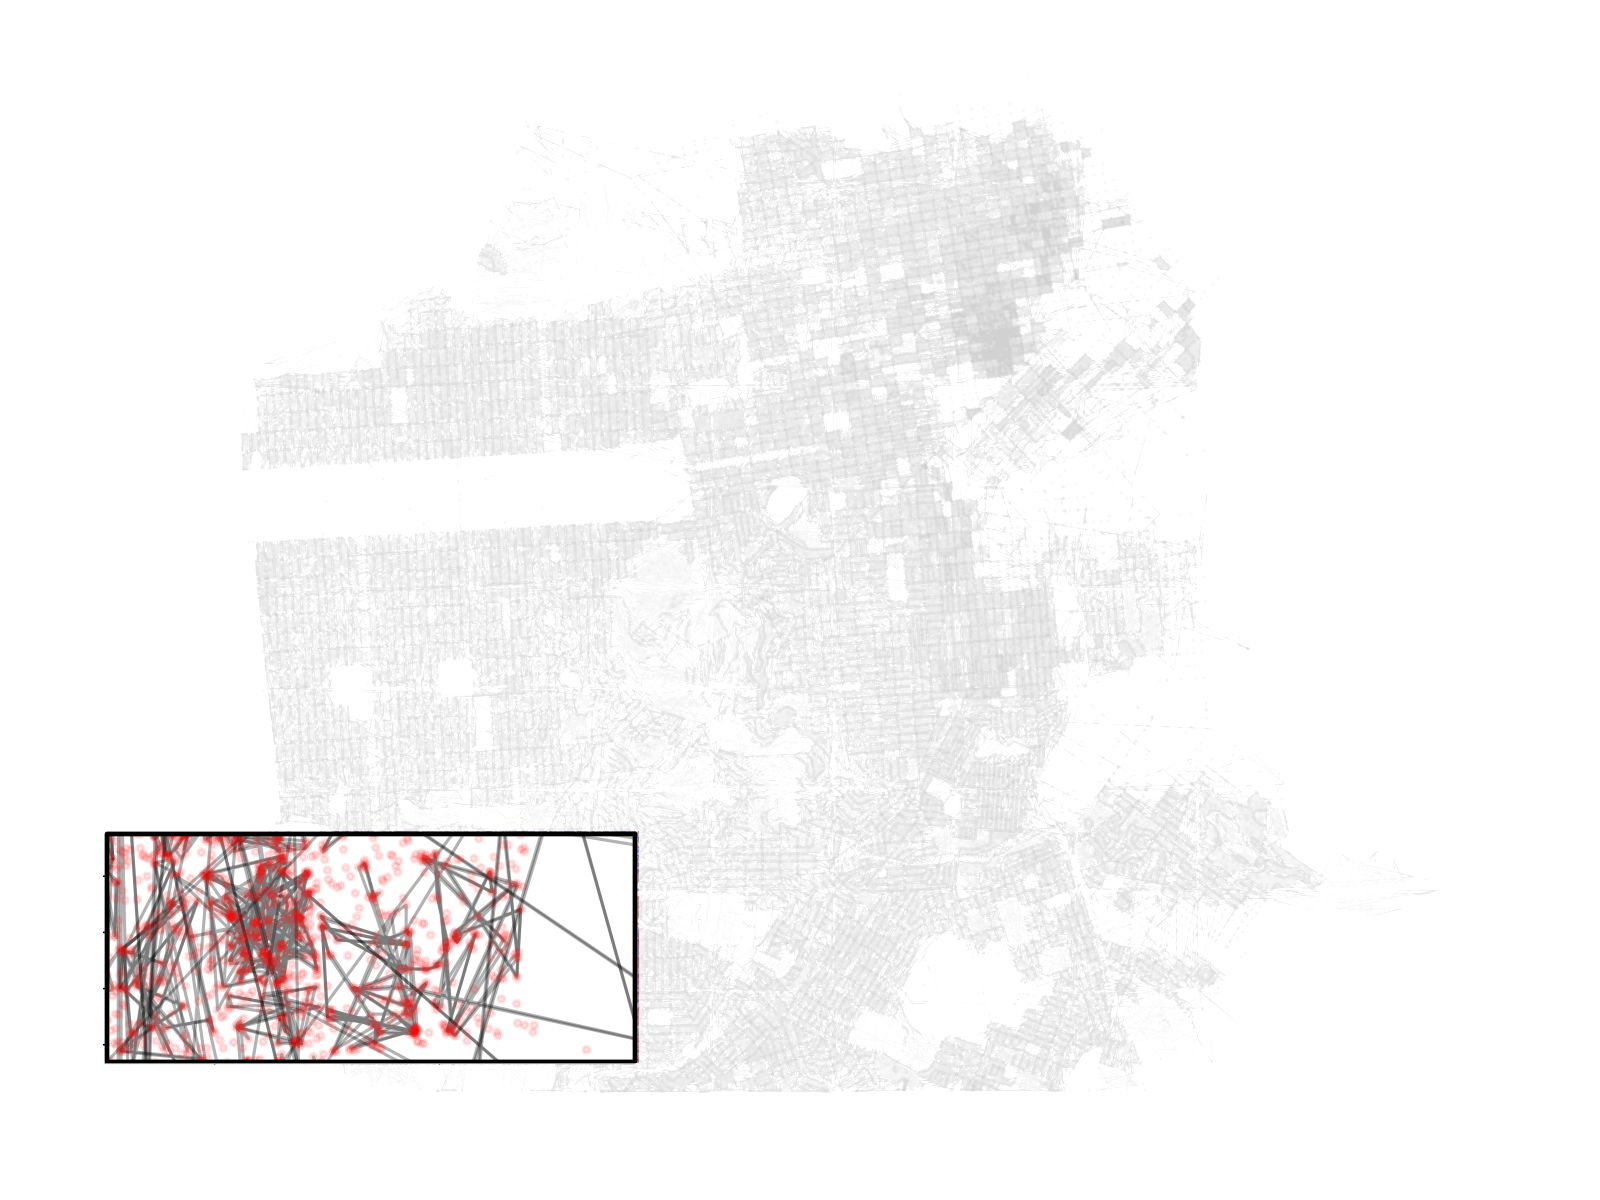
\includegraphics[width=\paperwidth]{graphics/sf_example}}
%\usebackgroundtemplate{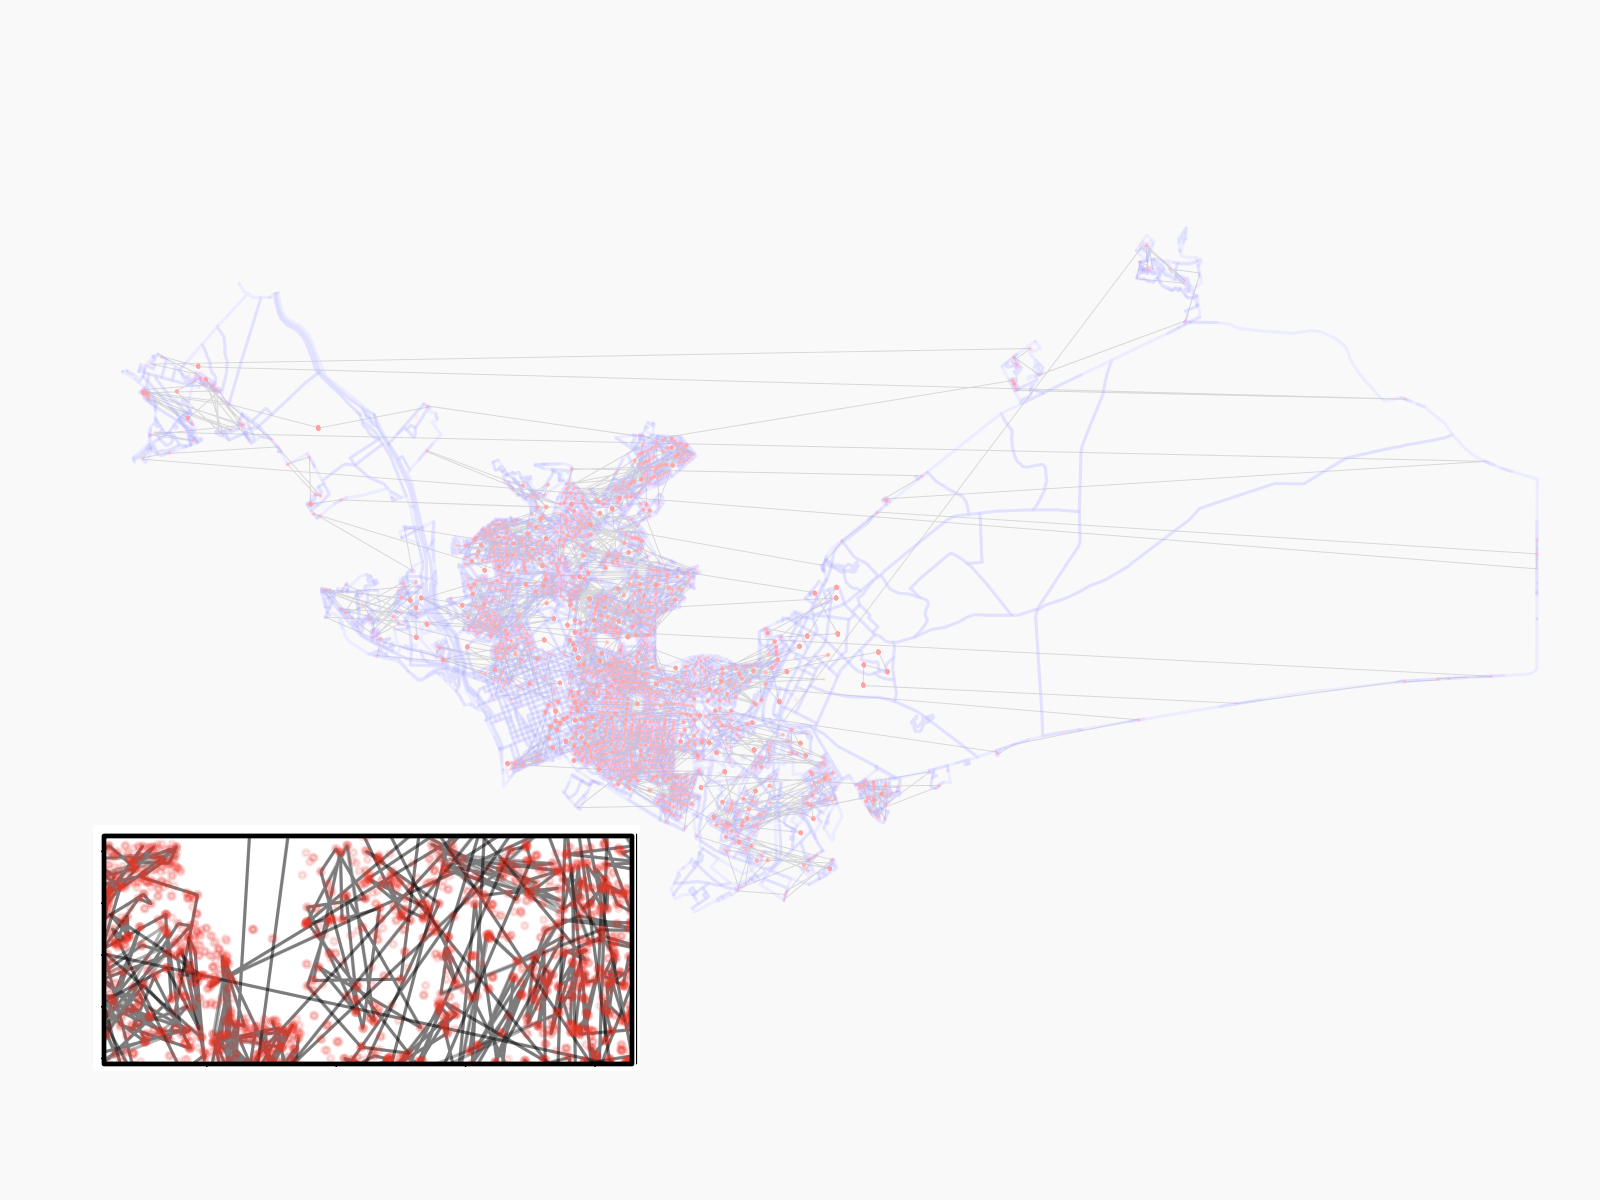
\includegraphics[width=\paperwidth]{graphics/southcarolina2.png}}
\usebackgroundtemplate{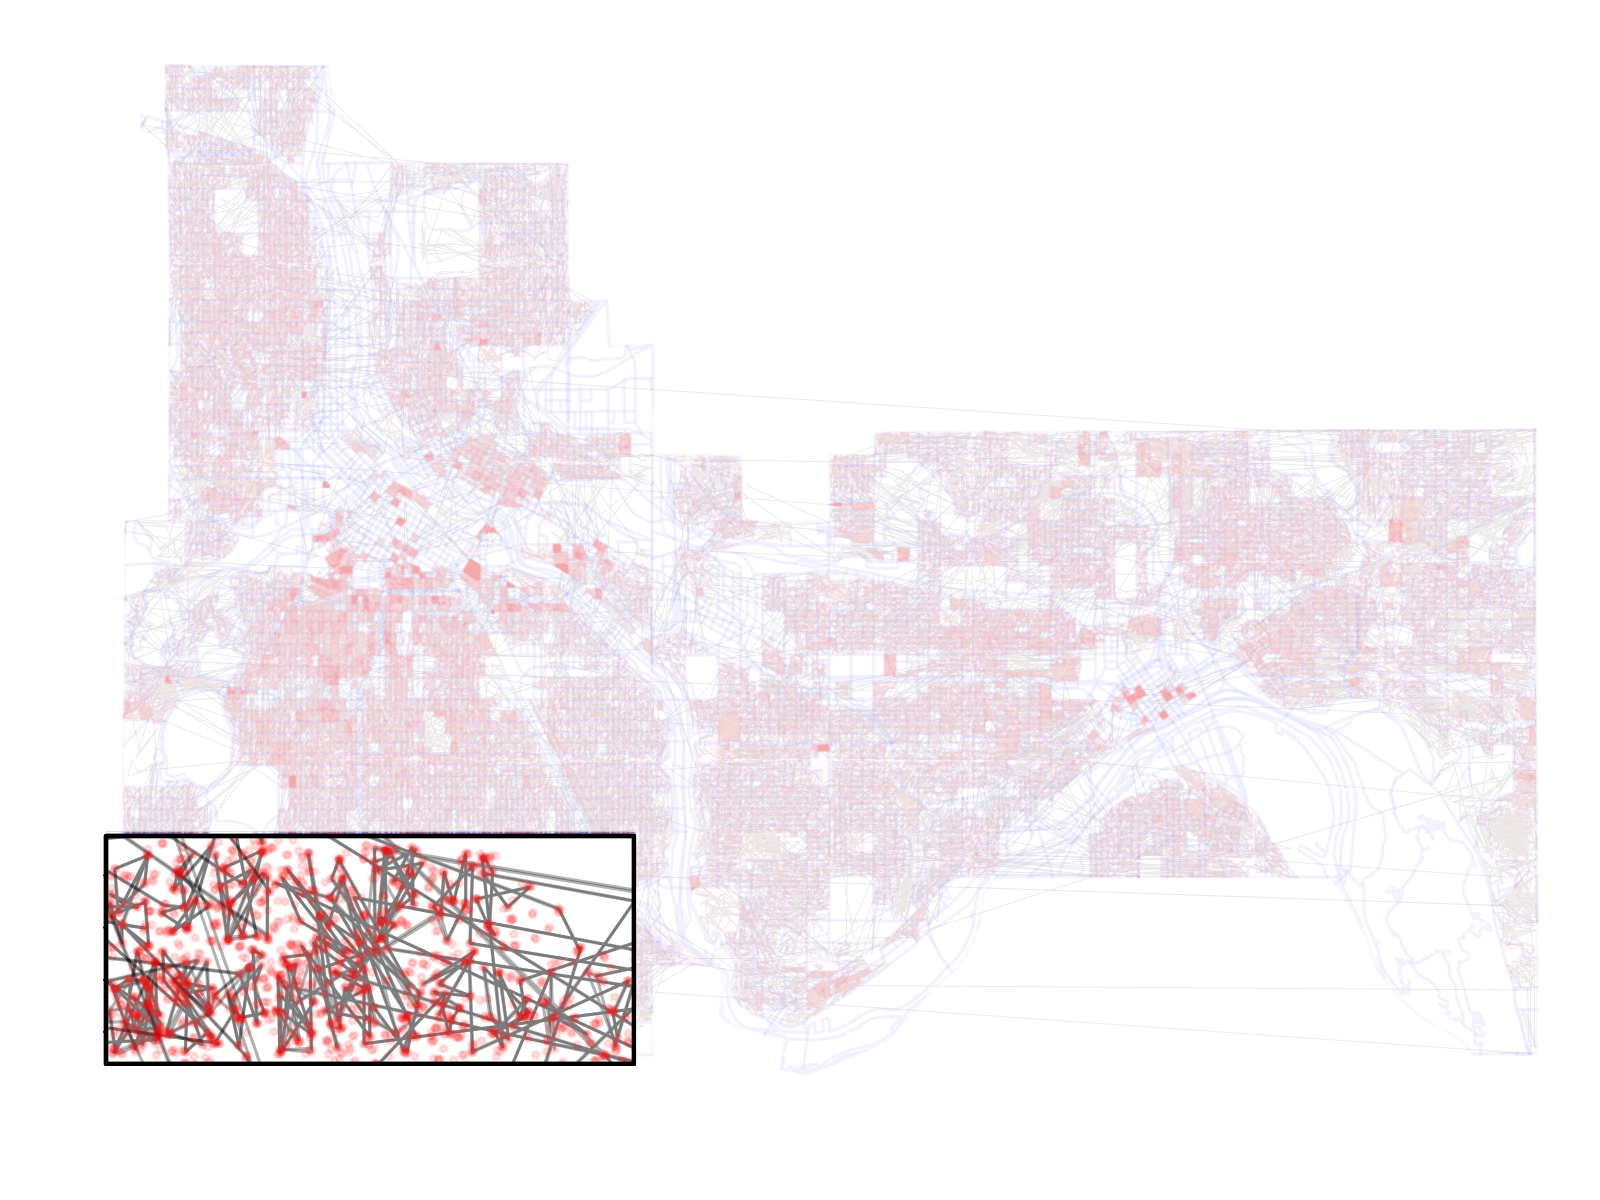
\includegraphics[width=1.1\paperwidth]{graphics/minn.png}}
\begin{frame}[plain]
  \titlepage
\end{frame}
}



%----------- slide --------------------------------------------------%


%----------- section ----------------------------------------------%
\section{Introduction}
%----------- section ----------------------------------------------%




%----------- slide --------------------------------------------------%
%{
%\usebackgroundtemplate{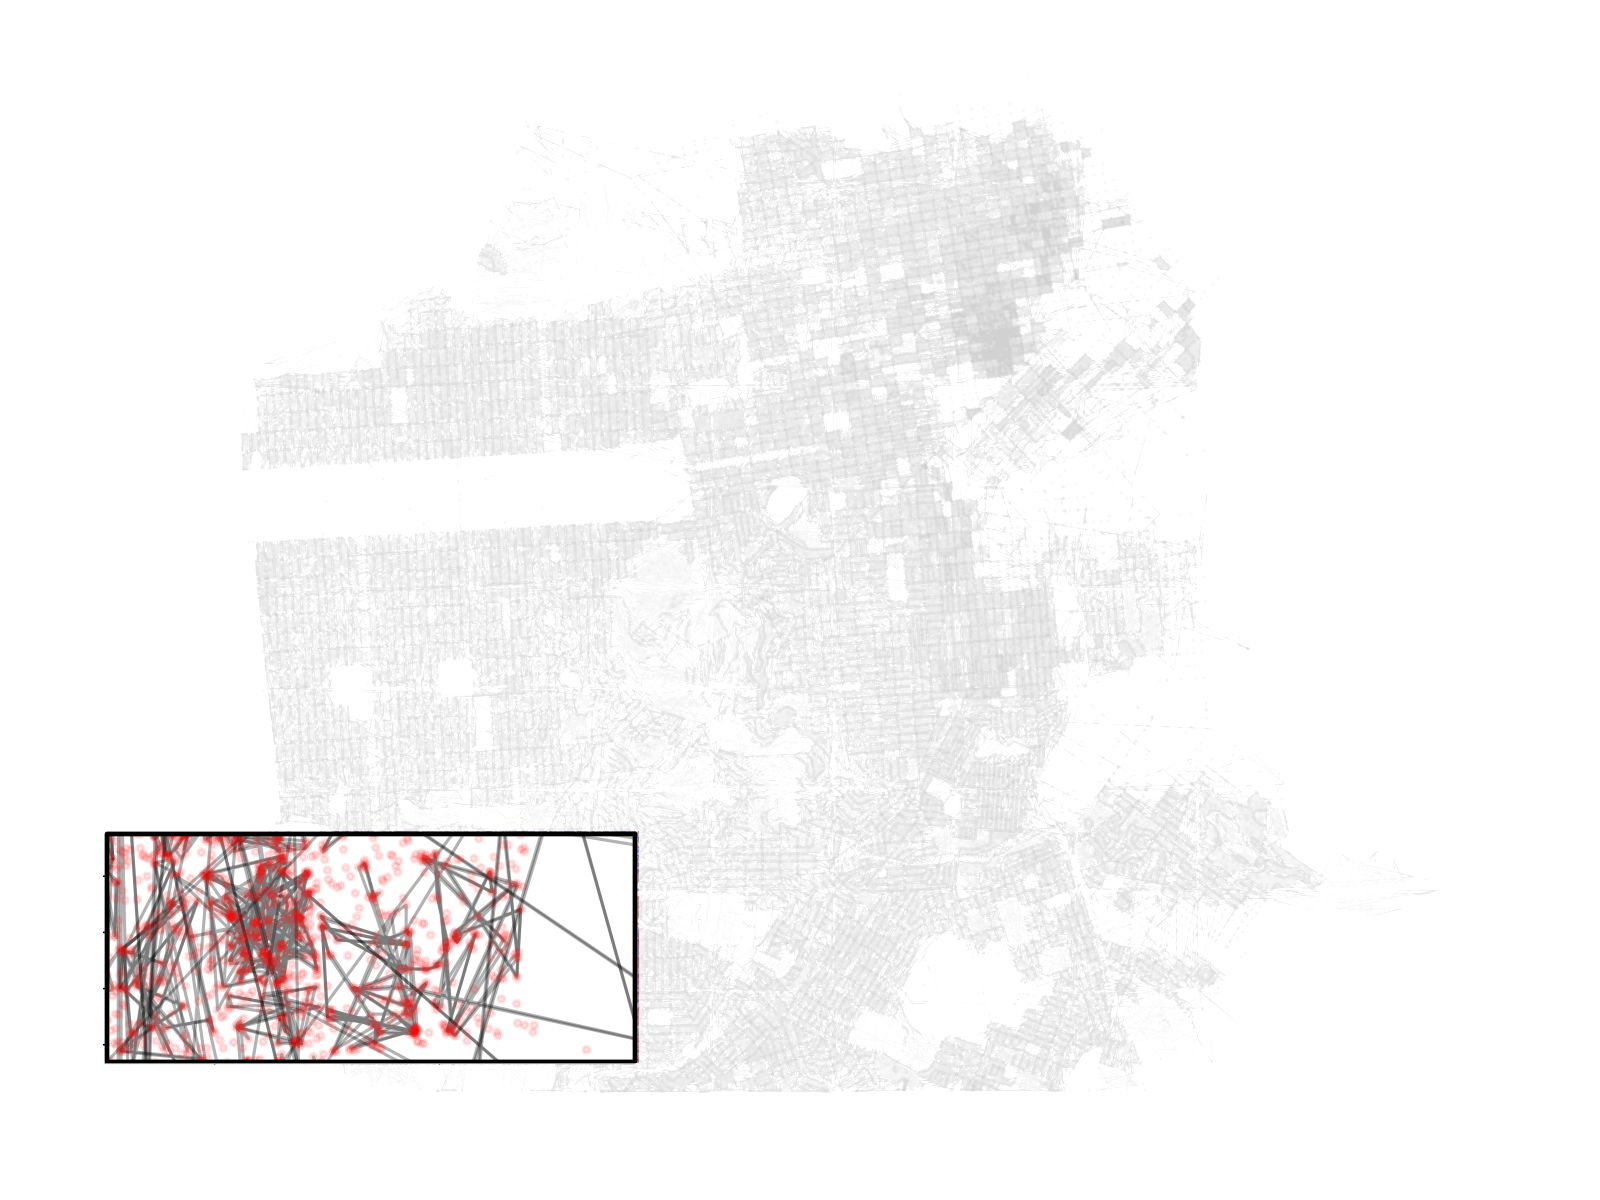
\includegraphics[width=\paperwidth]{graphics/sf_example}}
%\usebackgroundtemplate{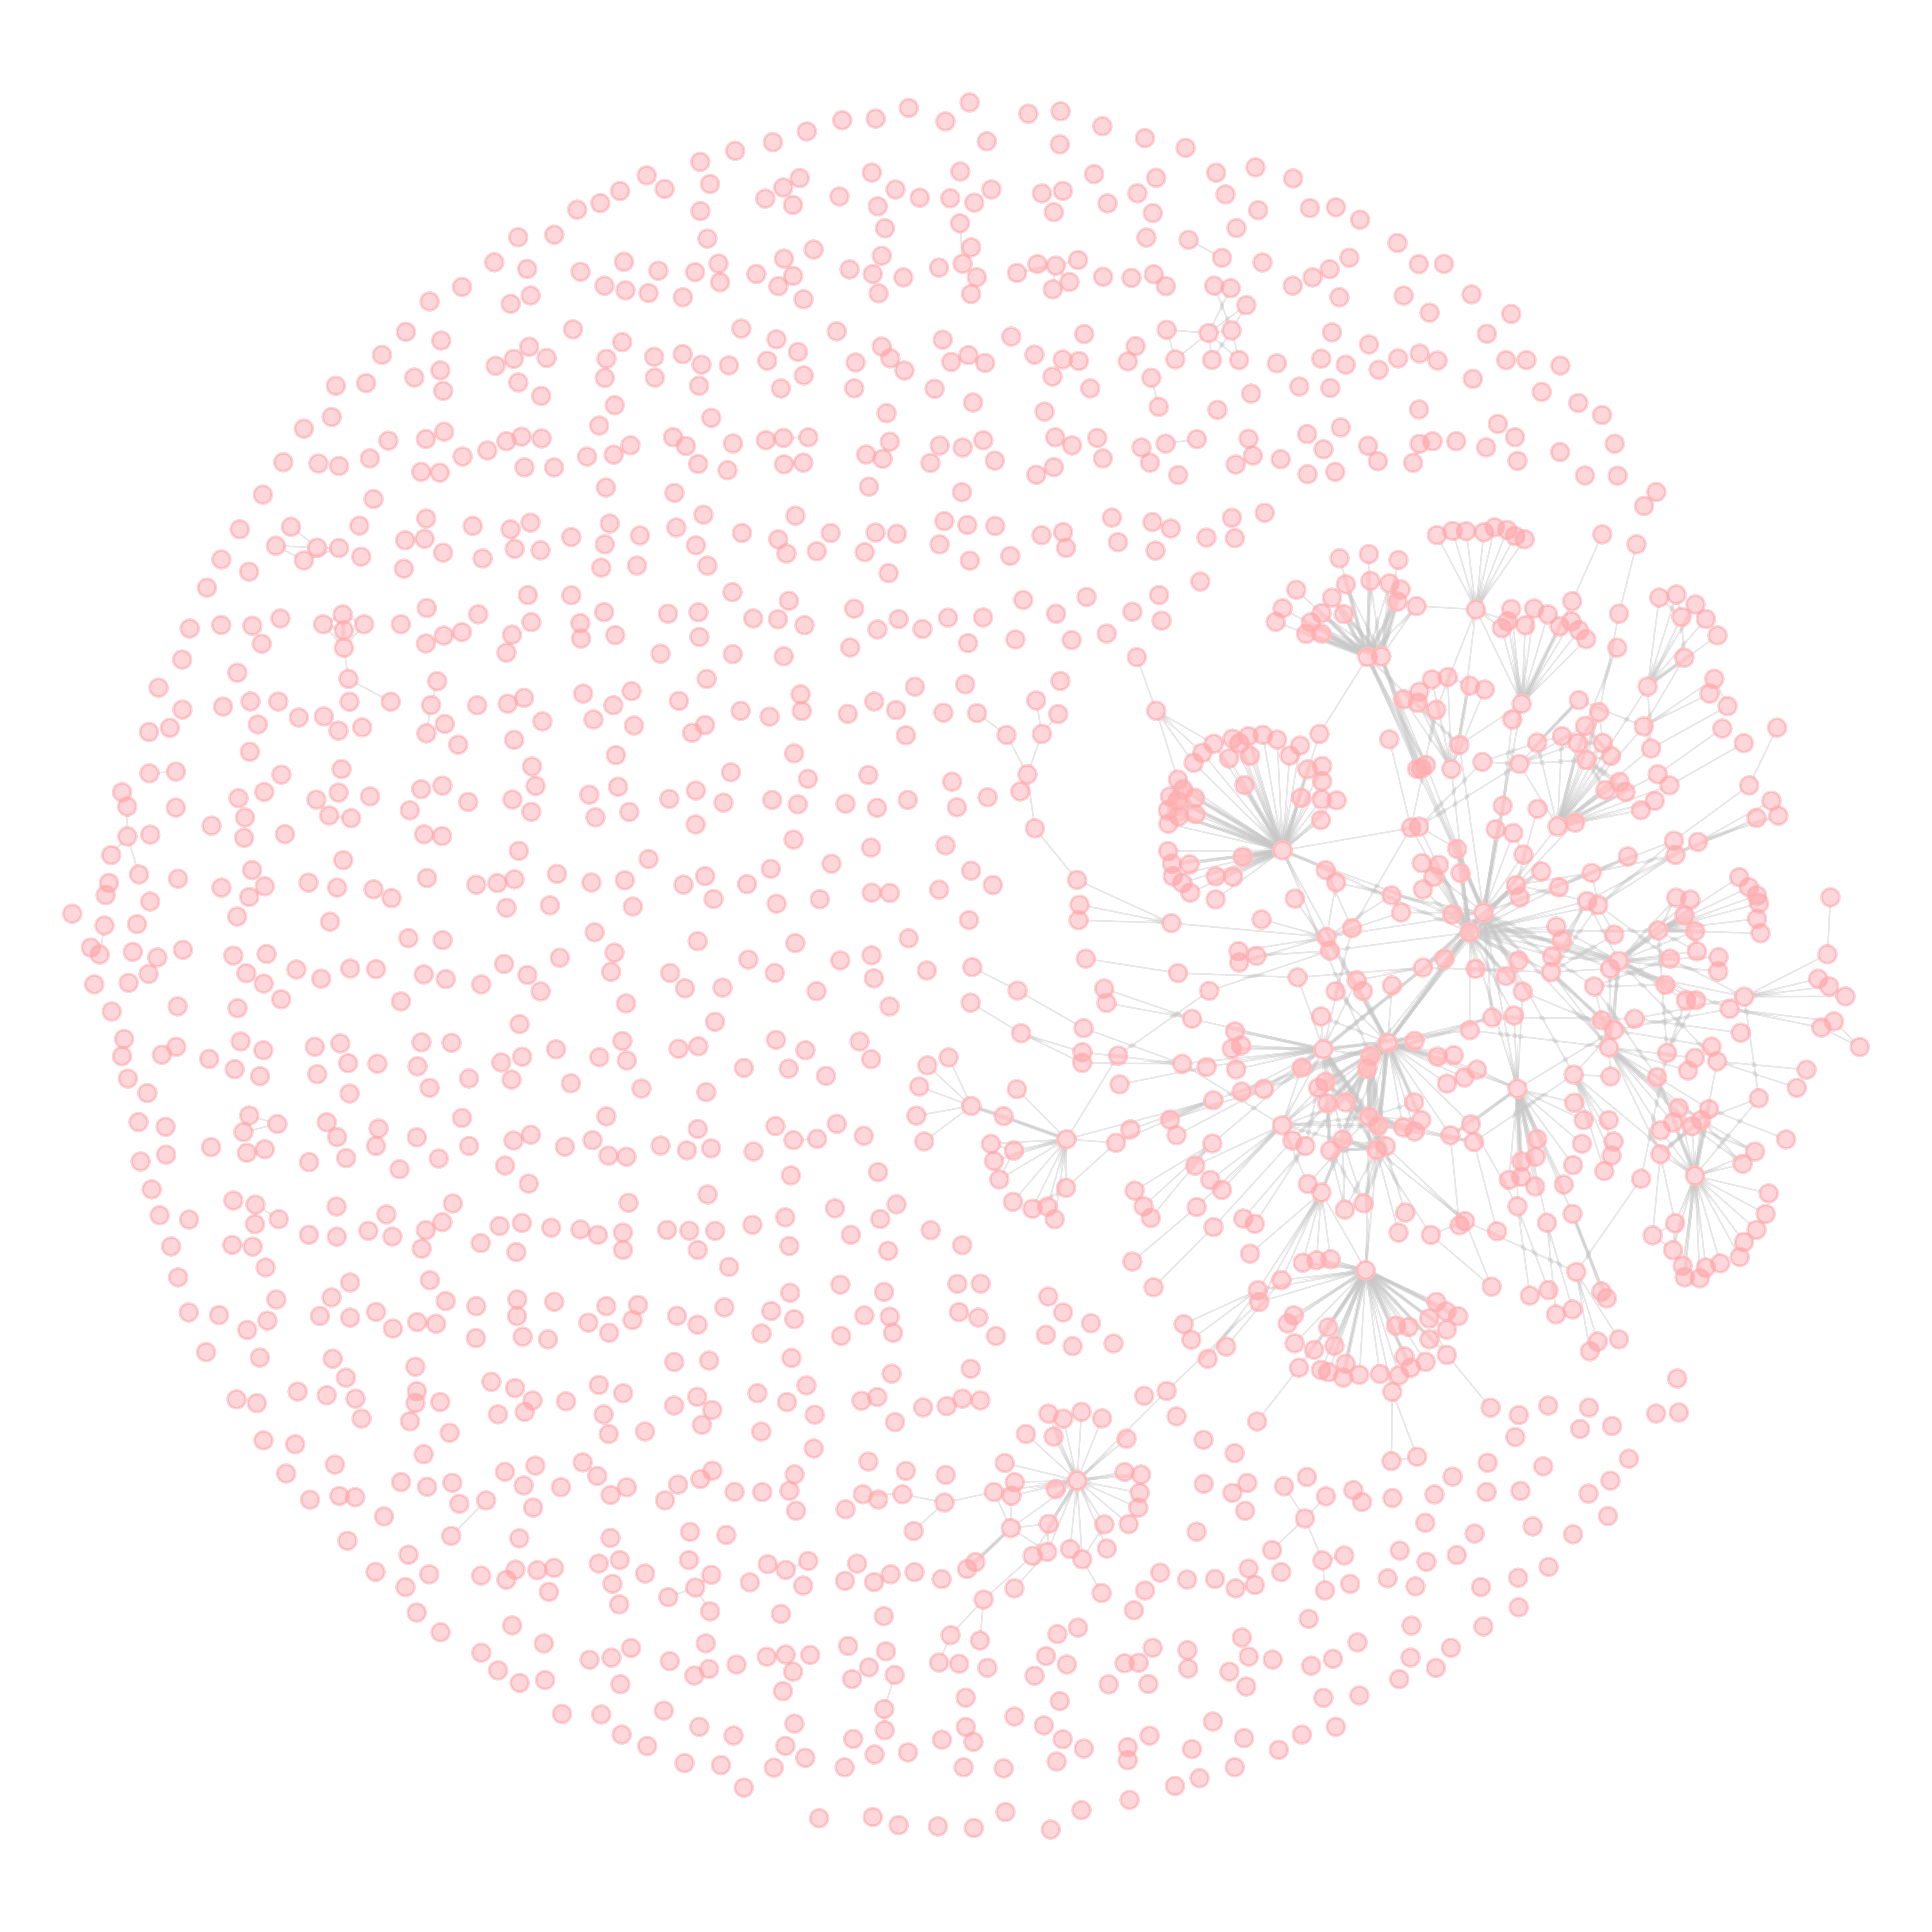
\includegraphics[width=.7\paperwidth]{graphics/katrinaplot.png}}
\begin{frame}[t]{Road Map}

\begin{textblock*}{100mm}(20mm,0.3\textheight)
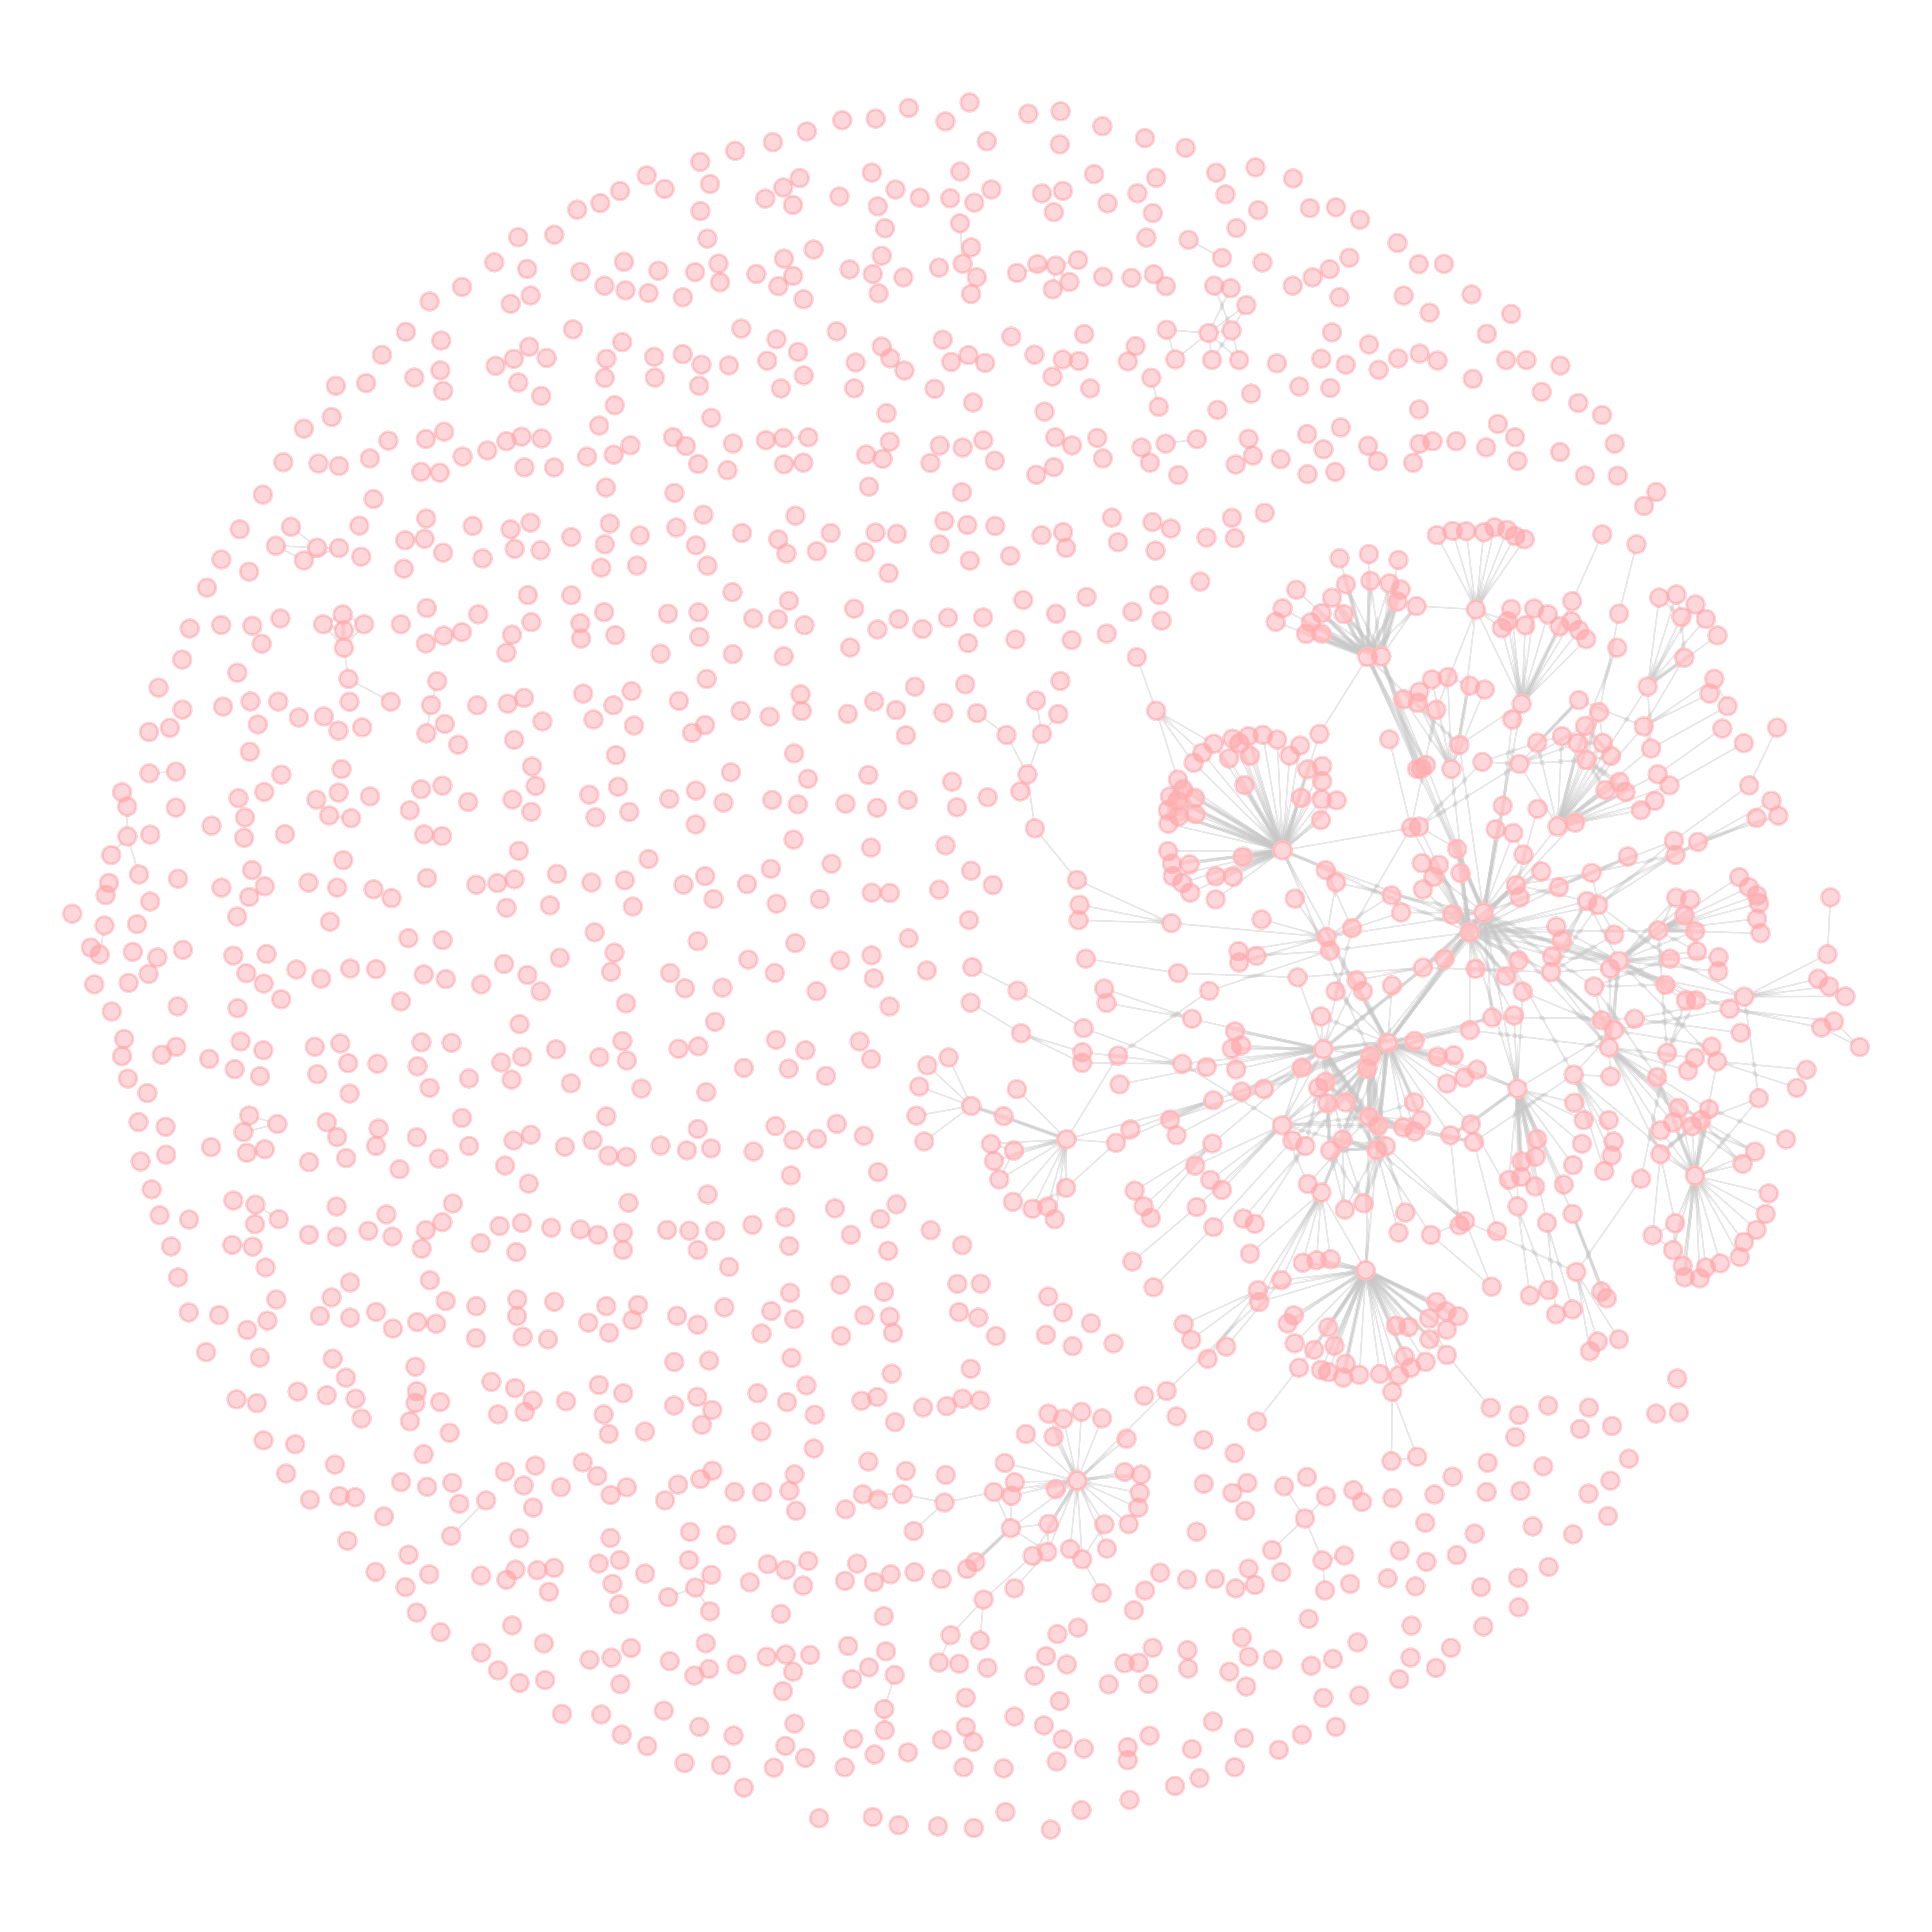
\includegraphics[width=\paperwidth]{graphics/katrinaplot.png}
\end{textblock*}

\begin{textblock*}{100mm}(20mm,0.3\textheight)
\begin{center}
\begin{itemize}
\item[\textbf{1)}] Overview of Population/Network Processes
\item[\textbf{2)}] Examples
\item[\textbf{3)}] A Model for Dynamic Networks with Population Processes
\item[\textbf{4)}] Empirical Example
\item[\textbf{5)}] Further Reading
\end{itemize}
\end{center}
\end{textblock*}

%----------- Fix name --------------------------------------------------%
\begin{textblock*}{100mm}(4mm,1.02\textheight)

\includegraphics[width=20mm,height=5mm ]{graphics/white.png}
\end{textblock*}

\begin{textblock*}{100mm}(4mm,1.02\textheight)
\emph{\tiny{\darkblue{Zack W Almquist, UMN}}}
\end{textblock*}
%----------- Fix name --------------------------------------------------%

\end{frame}
%}
%----------- slide --------------------------------------------------%


%----------- slide --------------------------------------------------%
\begin{frame}[t]{Dynamic Networks with Population Processes}
\only<1>{

\begin{textblock*}{100mm}(15mm,0.2\textheight)
\Huge{Who Shows up to the Party?}
\end{textblock*}

\begin{textblock*}{85mm}(20mm,0.3\textheight)
%
\includegraphics[width=1\linewidth]{graphics/gameCocksNW.png}
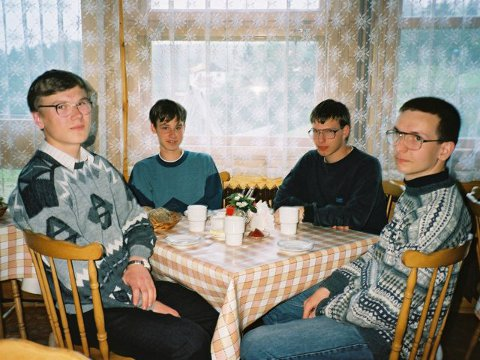
\includegraphics[width=1\linewidth]{graphics/spatial1.jpg}
\end{textblock*}

}
\only<2>{

\begin{textblock*}{100mm}(15mm,0.2\textheight)
\Huge{Who Shows up to the Party?}
\end{textblock*}

\begin{textblock*}{85mm}(20mm,0.3\textheight)
%
\includegraphics[width=1\linewidth]{graphics/gamecocks.jpg}
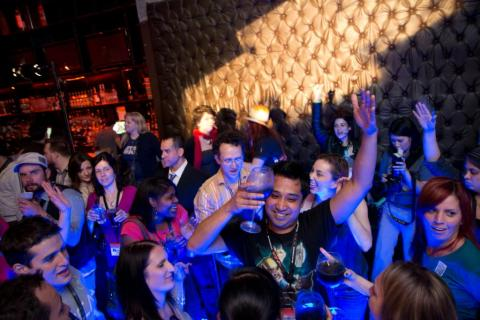
\includegraphics[width=1\linewidth]{graphics/party.jpg}
\end{textblock*}
}
%\only<3>{
%\begin{textblock*}{100mm}(15mm,0.2\textheight)
%\Huge{Who Shows up to the Party?}
%\end{textblock*}

%\begin{textblock*}{85mm}(20mm,0.3\textheight)
%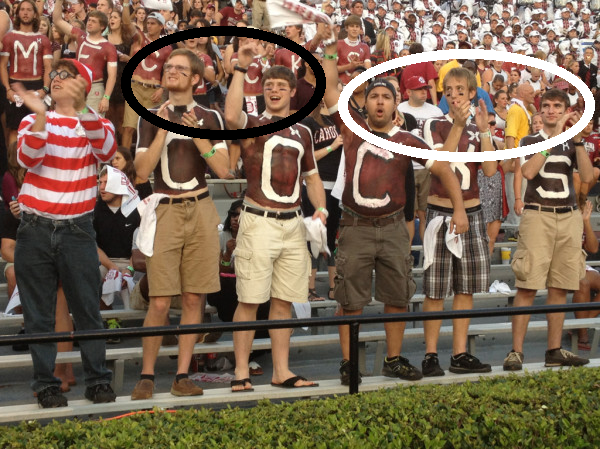
\includegraphics[width=1\linewidth]{graphics/gameCocksGroup.png}
%\end{textblock*}
%}
\only<3>{
\begin{block}{Dynamic Populations}
\begin{itemize}
\item \dd{Educational settings}
\vspace{-.3cm}
\begin{columns}
\begin{column}{0.4\textwidth}
\begin{itemize}
\item Classrooms
\item Yearly turnover
\end{itemize}
\end{column}
\begin{column}{0.4\textwidth}
\begin{itemize}
\item e.g., \citet{coleman61,hodgkinson85,feldman72}%,levine89} %% COLMAN
\end{itemize}
\end{column}
\end{columns}
\item \dd{Human societies}
\vspace{-.3cm}
\begin{columns}
\begin{column}{0.4\textwidth}
\begin{itemize}
\vspace{.2cm}
\item Communication
\item Interaction
\end{itemize}
\end{column}
\begin{column}{0.4\textwidth}
\begin{itemize}
\item e.g., \citet{mayhew76,chase80} %% COLMAN
\end{itemize}
\end{column}
\end{columns}
\item \dd{Demography}
\vspace{-.2cm}
\begin{columns}
\begin{column}{0.4\textwidth}
\begin{itemize}
\item Forecasting
\item Birth/Death/Mobility
\end{itemize}
\end{column}
\begin{column}{0.4\textwidth}
\begin{itemize}
\item e.g., \citet{lee87,lee92} %% Demography cites
\end{itemize}
\end{column}
\end{columns}
\item \dd{Organizations}
\vspace{-.3cm}
\begin{columns}
\begin{column}{0.4\textwidth}
\vspace{-.2cm}
\begin{itemize}
\item Org. Demography
\item Org. Ecology
\end{itemize}
\end{column}
\begin{column}{0.4\textwidth}
\begin{itemize}
\item e.g., \citet{hannan77,hannan84,anderton83b,romo95} %% Organization Class
\end{itemize}
\end{column}
\end{columns}
\end{itemize}
\end{block}
}
\only<4>{
\vspace{-.2cm}
\begin{block}{Dynamic Networks}
\begin{itemize}
\item \dd{Educational settings}
\vspace{-.2cm}
\begin{columns}
\begin{column}{0.4\textwidth}
\begin{itemize}
\item Friendship over time
\item Influence networks (e.g., smoking)
\end{itemize}
\end{column}
\begin{column}{0.4\textwidth}
\begin{itemize}
\item e.g., \citet{newcomb61,nordlie58,mercken10}  %% COLMAN
\end{itemize}
\end{column}
\end{columns}
\item \dd{Human societies}
\vspace{-.3cm}
\begin{columns}
\begin{column}{0.4\textwidth}
\begin{itemize}
\item Communication
\item Interaction
\end{itemize}
\end{column}
\begin{column}{0.4\textwidth}
\begin{itemize}
\item e.g.,  \citet{vanderijt11,dogan09,buskens08} %% COLMAN
\end{itemize}
\end{column}
\end{columns}
\vspace{-.2cm}
\item \dd{Demography}
\vspace{-.3cm}
\begin{columns}
\begin{column}{0.4\textwidth}
\begin{itemize}
\item Sexual contact networks
\item Kinship networks
\end{itemize}
\end{column}
\begin{column}{0.4\textwidth}
\begin{itemize}
\item e.g.,  \citet{entwisle07,fischer82,boyd89}%% Demography cites
\end{itemize}
\end{column}
\end{columns}
\item \dd{Organizations}
\vspace{-.2cm}
\begin{columns}
\begin{column}{0.4\textwidth}
\begin{itemize}
\item Collaboration 
\item Composition
\end{itemize}
\end{column}
\begin{column}{0.4\textwidth}
\begin{itemize}
\item e.g., \citet{carley99,butts09a,mintz81} %% Organization Class
\end{itemize}
\end{column}
\end{columns}
\end{itemize}
\end{block}
}
\only<5>{
\begin{block}{Dynamic Networks with Dynamic Populations}
\begin{itemize}
\item \dd{Sexual contact networks}
\vspace{-.4cm}
\begin{columns}[t]
\begin{column}{0.4\textwidth}
\begin{itemize}
\item HIV Transmission 
\item e.g., Add Health, Uganda
\end{itemize}
\end{column}
\begin{column}{0.4\textwidth}
\begin{itemize}
\item e.g., \citet{bearman04,morris97}%% COLMAN
\end{itemize}
\end{column}
\end{columns}
\item \dd{Organizational collaboration during disasters}
\vspace{-.4cm}
\begin{columns}[t]
\begin{column}{0.4\textwidth}
\begin{itemize}
\item Disaster response
\item e.g., Hurricane Katrina, 9/11
\end{itemize}
\end{column}
\begin{column}{0.4\textwidth}
\begin{itemize}
\item e.g.,   \citet{butts.acton.marcum:2008a,butts08b} 
\end{itemize}
\end{column}
\end{columns}
\item \dd{Informal groups}
\vspace{-.4cm}
\begin{columns}[t]
\begin{column}{0.4\textwidth}
\begin{itemize}
\item Interaction
\item e.g., movements, gangs
\end{itemize}
\end{column}
\begin{column}{0.4\textwidth}
\begin{itemize}
\item e.g.,   \citet{freeman88,freeman92}%% Demography cites
\end{itemize}
\end{column}
\end{columns}
\end{itemize}
\end{block}
}
\end{frame}
%----------- slide --------------------------------------------------%

%\begin{frame}[t]{Population and Network Processes}
%\only<1>{
%\begin{textblock*}{50mm}(15mm,0.4\textheight)
%\begin{block}{Demographers}
%Largely focuses on \dots
%\end{block}
%\end{textblock*}
%}
%\only<2>{
%\begin{textblock*}{50mm}(15mm,0.4\textheight)
%\begin{block}{Demographers}
%\begin{itemize}
%\item (Population level) Fertility 
%\item (Population level) Mortality
%\item (Population level) Migration
%\end{itemize}
%\end{block}
%\end{textblock*}
%}
%\only<3>{
%\begin{textblock*}{50mm}(15mm,0.4\textheight)
%\begin{block}{Demographers}
%\end{block}
%\end{textblock*}
%}

%\only<1>{
%\begin{textblock*}{50mm}(70mm,0.4\textheight)
%\begin{block}{Social Networkers}
%Largely focuses on \dots
%\end{block}
%\end{textblock*}
%}
%\only<2>{
%\begin{textblock*}{50mm}(70mm,0.4\textheight)
%\begin{block}{Social Networkers}
%\end{block}
%\end{textblock*}
%}

%\only<3>{
%\begin{textblock*}{50mm}(70mm,0.4\textheight)
%\begin{block}{Social Networkers}
%\begin{itemize}
%\item Tie Creation
%\item Tie Dissolution
%\item (Processes that lead to) Structural Patterns
%\end{itemize}
%\end{block}
%\end{textblock*}
%}

%\only<4>{
%\begin{textblock*}{100mm}(15mm,0.2\textheight)
%\begin{block}{But What Happens When These Processes Interact?}
%\begin{itemize}
%\item Sexual contact networks
%\begin{itemize}
%\item Disease spreads via contact
%\item This spread in turn influences the population process
%\item This in turn affects the network 
%\end{itemize}
%\item Organizational response to disasters
%\begin{itemize}
%\item Mass convergence
%\item Emergent coordination tasks
%\item Different organizations show up on different days
%\end{itemize}
%\item Informal groups
%\begin{itemize}
%\item Communication/interaction
%\item Information passing
%\item Different individuals on different days
%\end{itemize}
%\end{itemize}
%\end{block}
%\end{textblock*}
%}

%\end{frame}

%----------- slide --------------------------------------------------%
\begin{frame}{Overview of Classic Population and Network Processes}

\only<1>{
\begin{block}{}
This work looks to combine \alert{demographic} and \alert{network} processes, in order to better understand their \alert{interaction} on social phenomena (e.g., organizational collaboration, sexual contact networks, informal group processes \dots)
\end{block}
}
\only<2>{
\begin{block}{}
\begin{itemize}
\item[1)] Population Processes
\item[2)] Network Processes
\end{itemize}
\end{block}
}
\end{frame}
%----------- slide --------------------------------------------------%


%----------- frame ----------------------------------------------%
\begin{frame}[t]{Classic Demographic Analysis}
\setbeamercovered{transparent}

\begin{block}{}
\centering
Population Processes
\end{block}


\begin{textblock*}{42mm}(16mm,0.4\textheight)
\begin{block}{}
\begin{itemize}
\item<1-2> Fertility
\begin{itemize}
\item[\birth{$\bullet$}]<1-2> Entry
\end{itemize}

\item<3-4> Mortality
\begin{itemize}
\item[\death{\textbf{X}}]<3-4> Exit
\end{itemize}
\item<5-7> Migration 
\begin{itemize}
\item[\mob{$\bullet$}]<5-7> Mobility
\end{itemize}
\end{itemize}
\end{block}
\end{textblock*}

\begin{textblock*}{62mm}(60mm,0.3\textheight)
\only<1>{
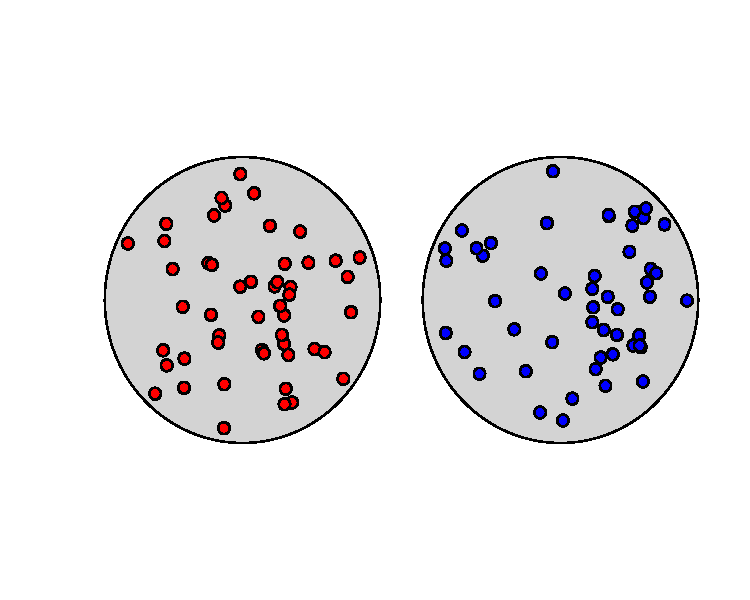
\includegraphics[width=1\linewidth]{graphics/pop1}
}
\only<2>{
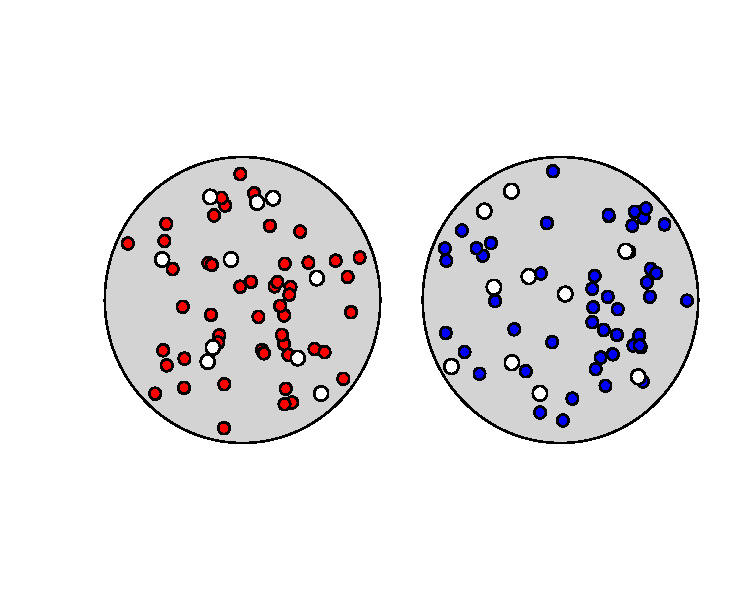
\includegraphics[width=1\linewidth]{graphics/pop2}
}
\only<3>{
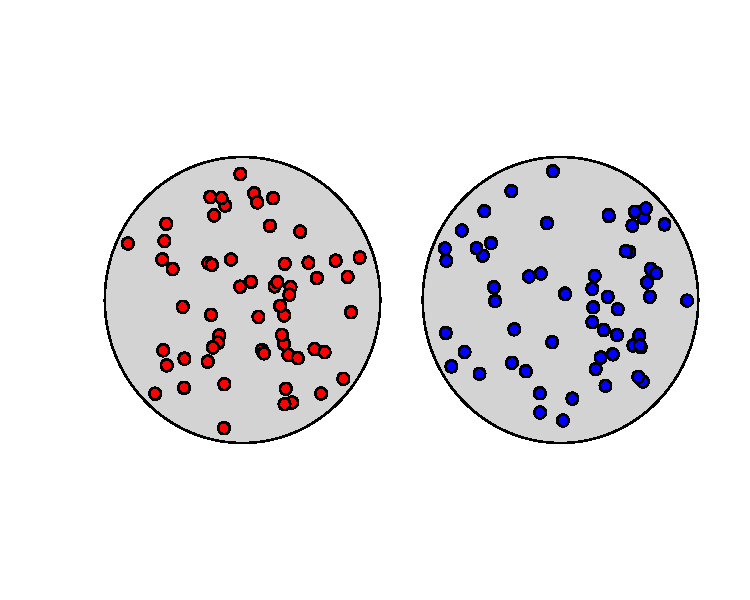
\includegraphics[width=1\linewidth]{graphics/pop3}
}
\only<4>{
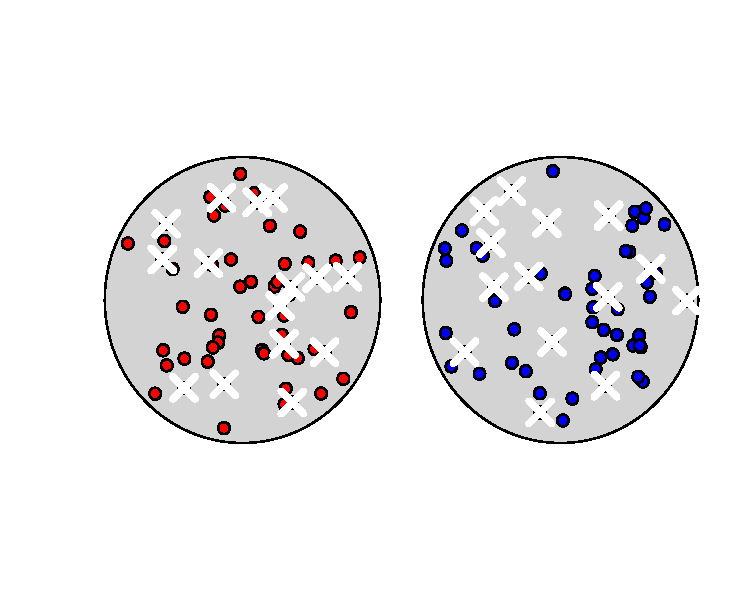
\includegraphics[width=1\linewidth]{graphics/pop4}
}

\only<5>{
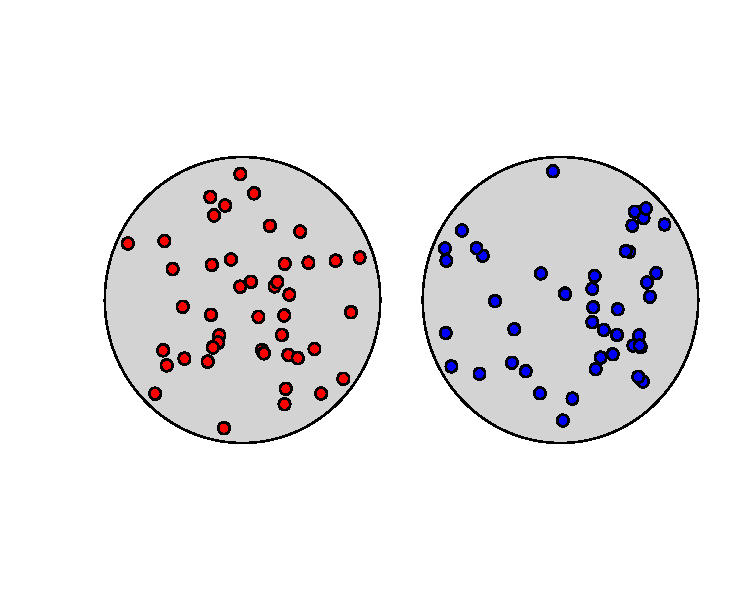
\includegraphics[width=1\linewidth]{graphics/pop5}
}
%\only<6>{
%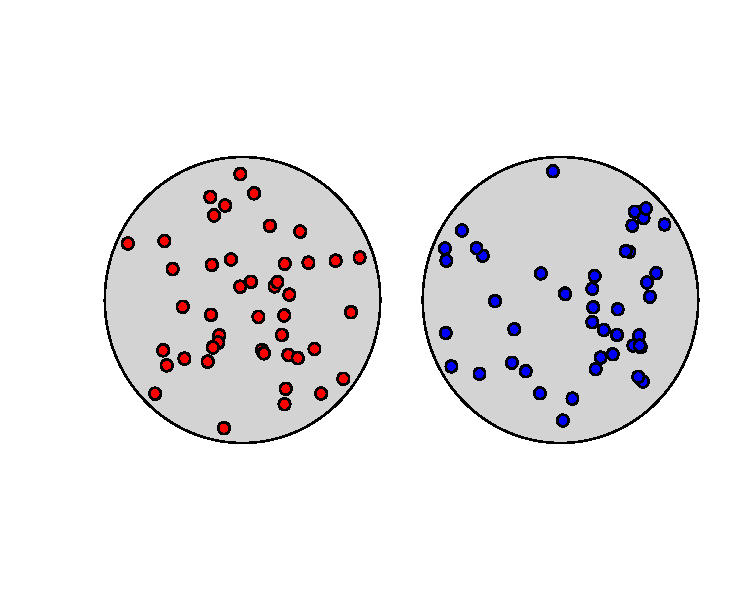
\includegraphics[width=1\linewidth]{graphics/pop6}
%}
\only<6>{
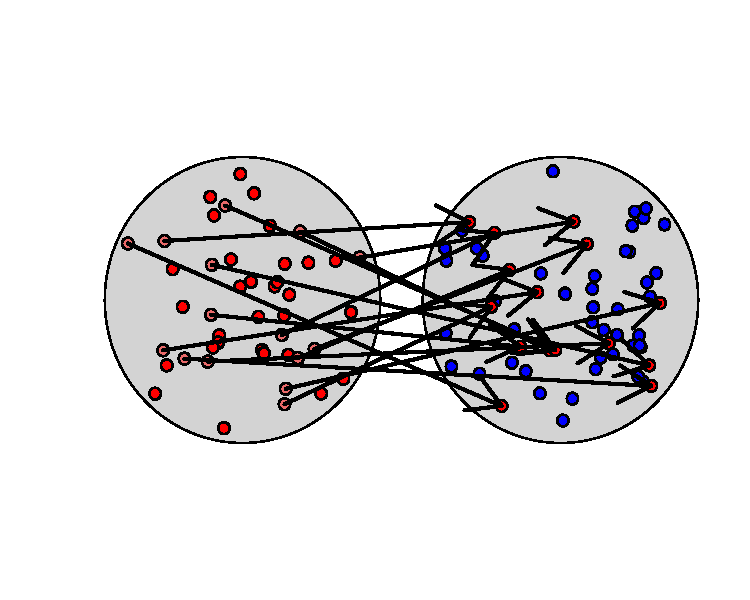
\includegraphics[width=1\linewidth]{graphics/pop7}
}
\only<7>{
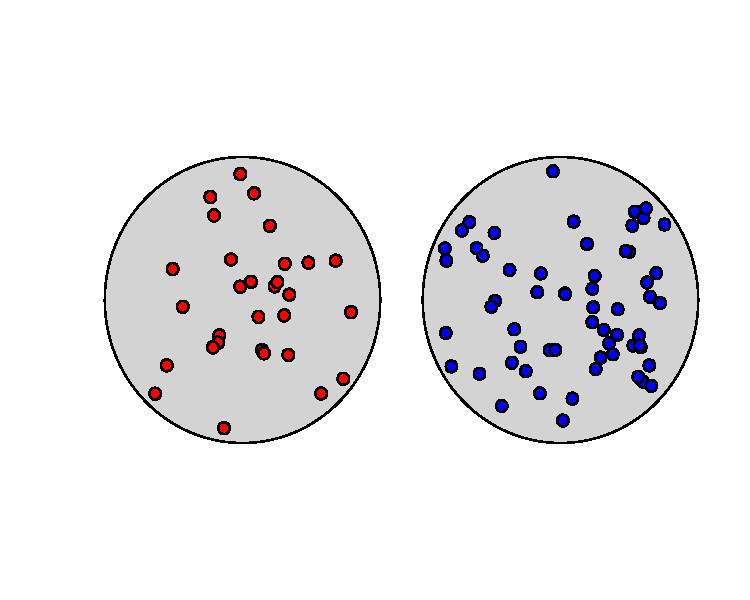
\includegraphics[width=1\linewidth]{graphics/pop8}
}
\end{textblock*}


\end{frame}
%----------- frame ----------------------------------------------%


%----------- frame ----------------------------------------------%
\begin{frame}[t]{Classic Network Analysis}
\setbeamercovered{transparent}

\begin{block}{}
\centering
Network Processes
\end{block}


\begin{textblock*}{42mm}(16mm,0.4\textheight)
\begin{block}{}
\begin{itemize}
\item<1-2> Tie Formation
\begin{itemize}
\item[\mob{$\bullet$}]<1-2> Adding ties
\end{itemize}
\item<3-4> Tie Dissolution
\begin{itemize}
\item[\mob{$\bullet$}]<3-4> Removing ties
\end{itemize}
\item<5-7> Structural Patterns
\begin{itemize}
\item[\mob{$\bullet$}]<6-7> e.g., Triadic closure
\end{itemize}
\end{itemize}
\end{block}
\end{textblock*}

\begin{textblock*}{62mm}(60mm,0.3\textheight)
\only<1>{
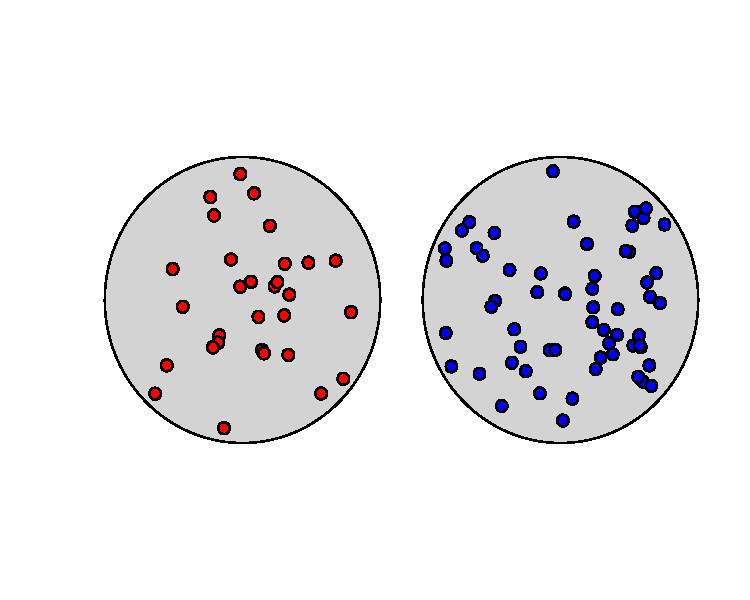
\includegraphics[width=1\linewidth]{graphics/net1}
}
\only<2>{
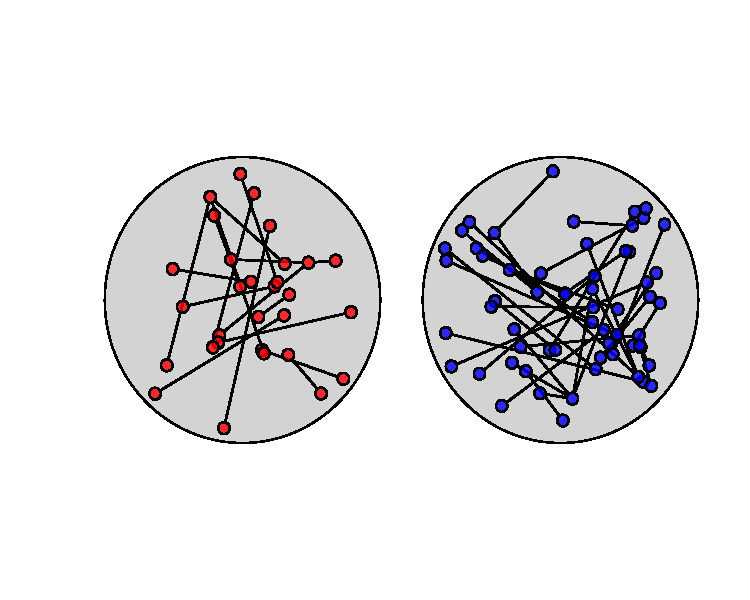
\includegraphics[width=1\linewidth]{graphics/net2}
}
\only<3>{
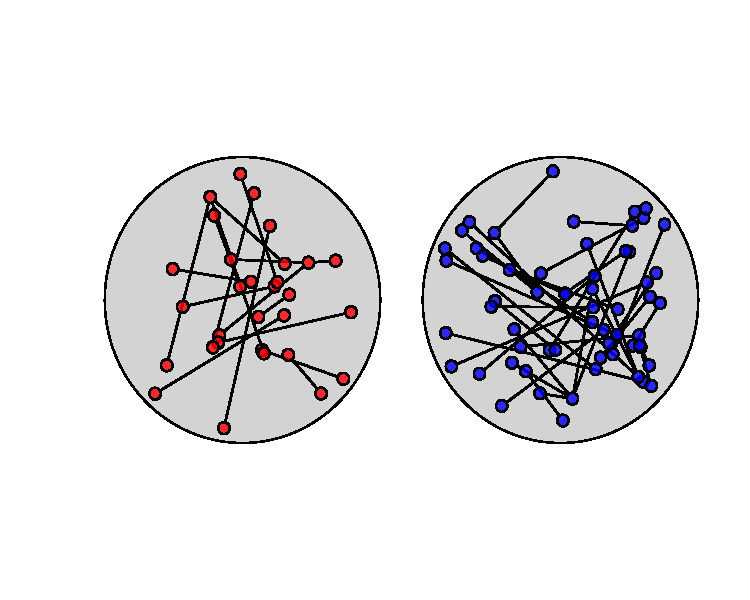
\includegraphics[width=1\linewidth]{graphics/net2}
}
\only<4>{
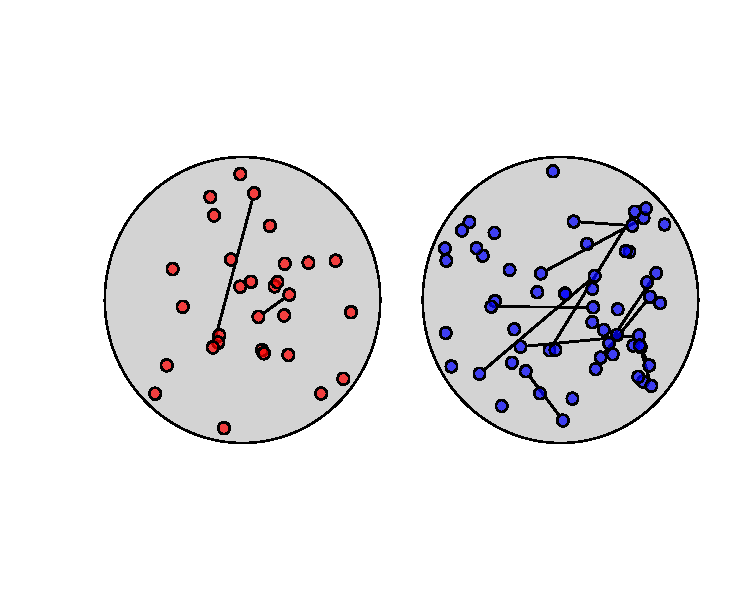
\includegraphics[width=1\linewidth]{graphics/net3}
}
\only<5>{
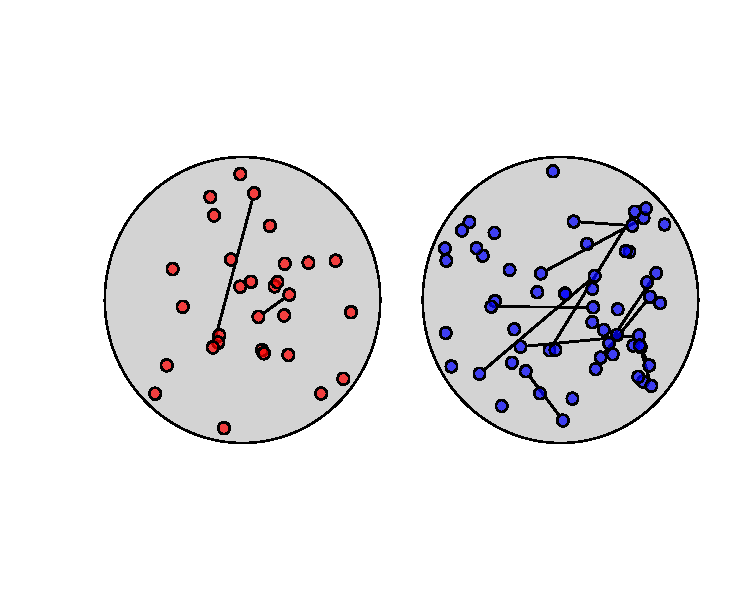
\includegraphics[width=1\linewidth]{graphics/net3}
}
\only<6>{
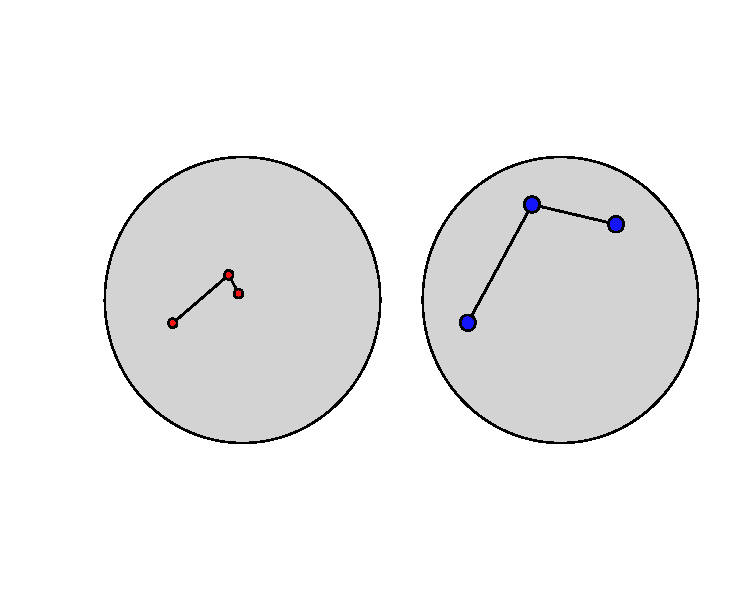
\includegraphics[width=1\linewidth]{graphics/net5}
}
\only<7>{
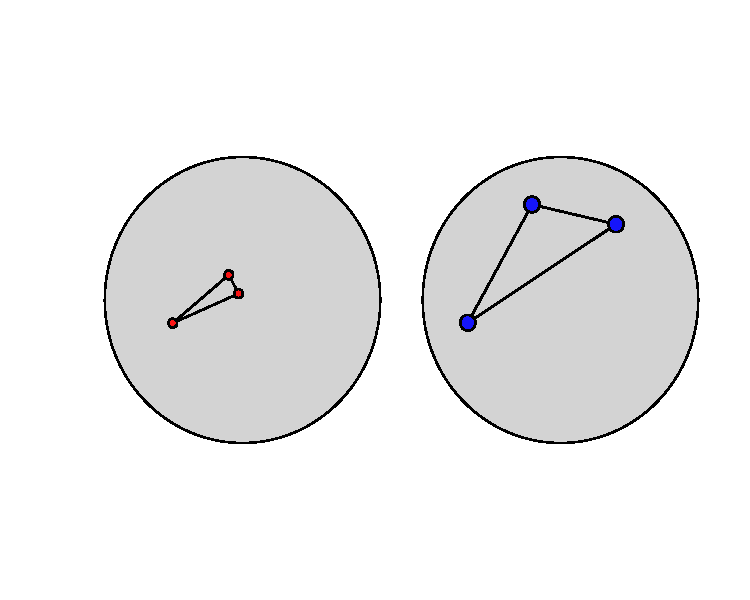
\includegraphics[width=1\linewidth]{graphics/net6}
}
\end{textblock*}

\end{frame}
%----------- frame ----------------------------------------------%

\begin{frame}[t]{Road Map}

\begin{textblock*}{100mm}(20mm,0.3\textheight)
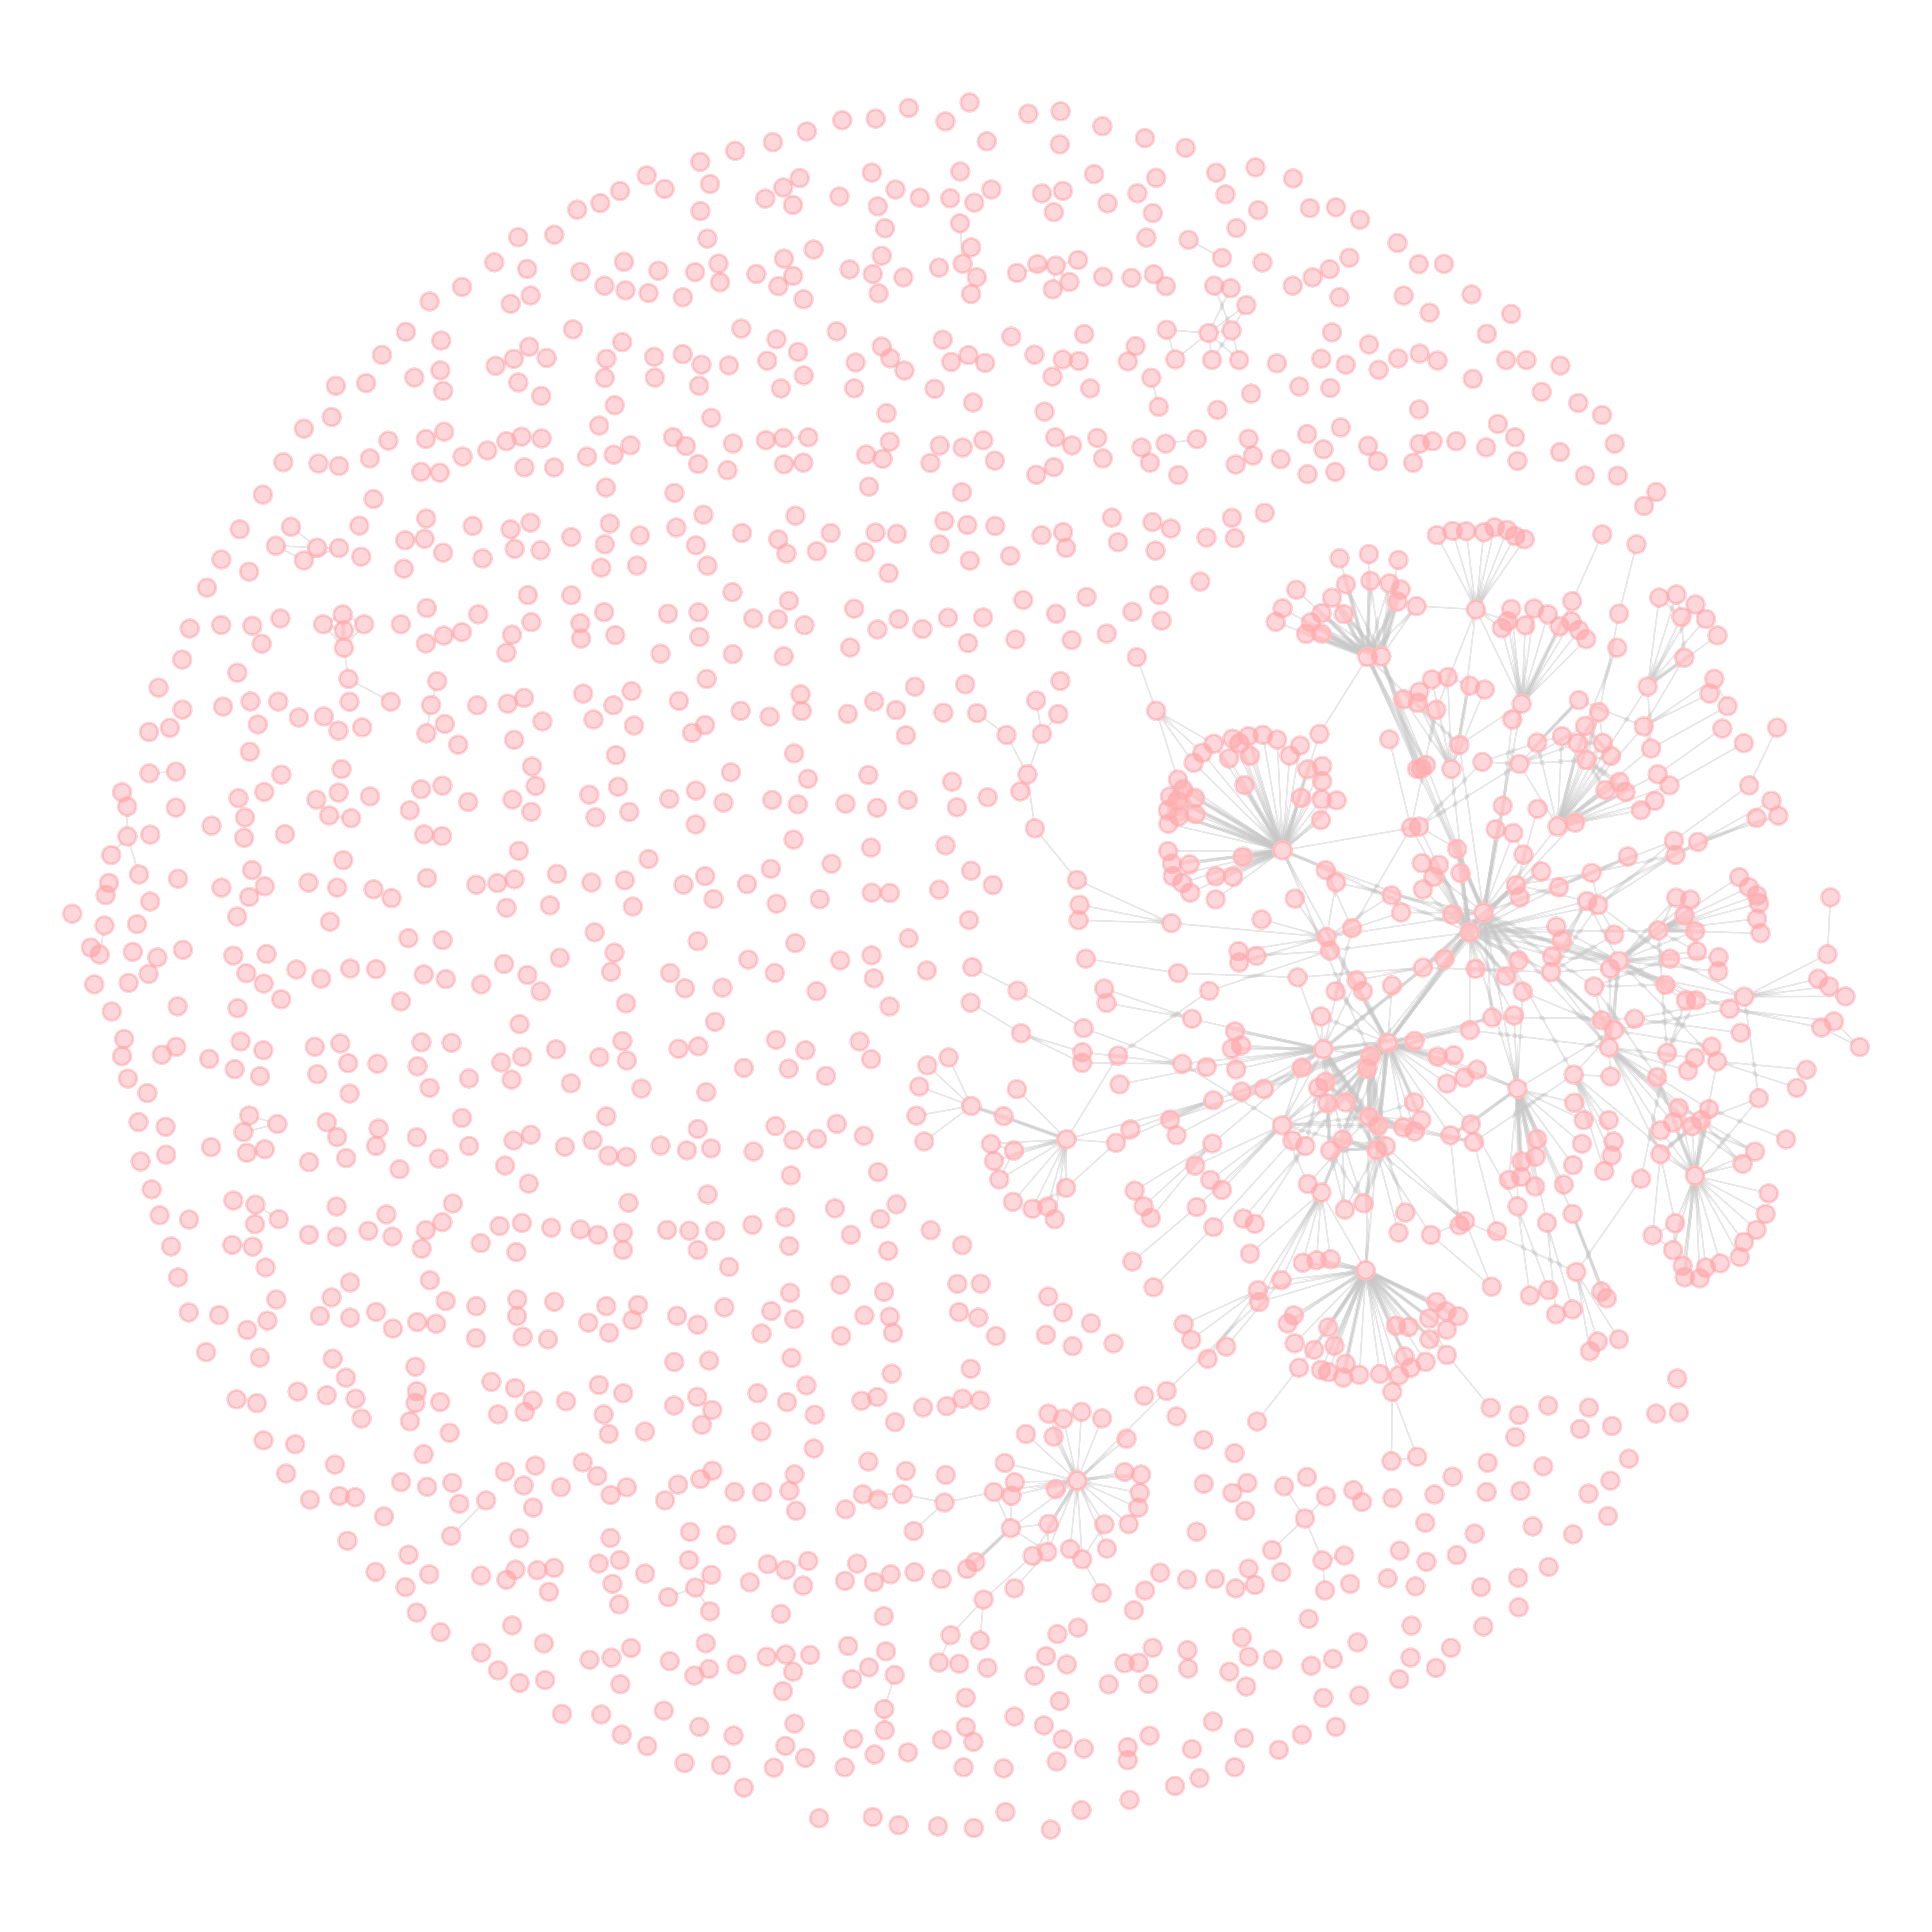
\includegraphics[width=\paperwidth]{graphics/katrinaplot.png}
\end{textblock*}

\begin{textblock*}{100mm}(20mm,0.3\textheight)
\begin{center}
\begin{itemize}
\item[\textcolor{light-gray}{\textbf{1)}}] \textcolor{light-gray}{Overview of Population/Network Processes}
\item[\textbf{2)}] Examples
\item[\textbf{3)}]  A Model for Dynamic Networks with Population Processes
\item[\textbf{4)}]  Empirical Example
\item[\textbf{5)}]  Further Reading
\end{itemize}
\end{center}
\end{textblock*}


%----------- Fix name --------------------------------------------------%
\begin{textblock*}{100mm}(4mm,1.02\textheight)

\includegraphics[width=20mm,height=5mm ]{graphics/white.png}
\end{textblock*}

\begin{textblock*}{100mm}(4mm,1.02\textheight)
\emph{\tiny{\darkblue{Zack W Almquist, UMN}}}
\end{textblock*}
%----------- Fix name --------------------------------------------------%

\end{frame}

%----------- frame ----------------------------------------------%
\begin{frame}[t]{Network Dynamics with Population Processes} 

\begin{textblock*}{100mm}(15mm,0.2\textheight)
\begin{block}{But What Happens When These Processes Interact?}
\begin{itemize}
\item Sexual contact networks
\begin{itemize}
\item Disease spreads via contact
\item This spread in turn influences the population process
\item This in turn affects the network 
\end{itemize}
\item Organizational response to disasters
\begin{itemize}
\item Mass convergence
\item Emergent coordination tasks
\item Different organizations show up on different days
\end{itemize}
\item Informal groups
\begin{itemize}
\item Communication/interaction
\item Information passing
\item Different individuals on different days
\end{itemize}
\end{itemize}
\end{block}
\end{textblock*}


\end{frame}
%----------- frame ----------------------------------------------%



\begin{frame}[t]{Road Map}

\begin{textblock*}{100mm}(20mm,0.3\textheight)
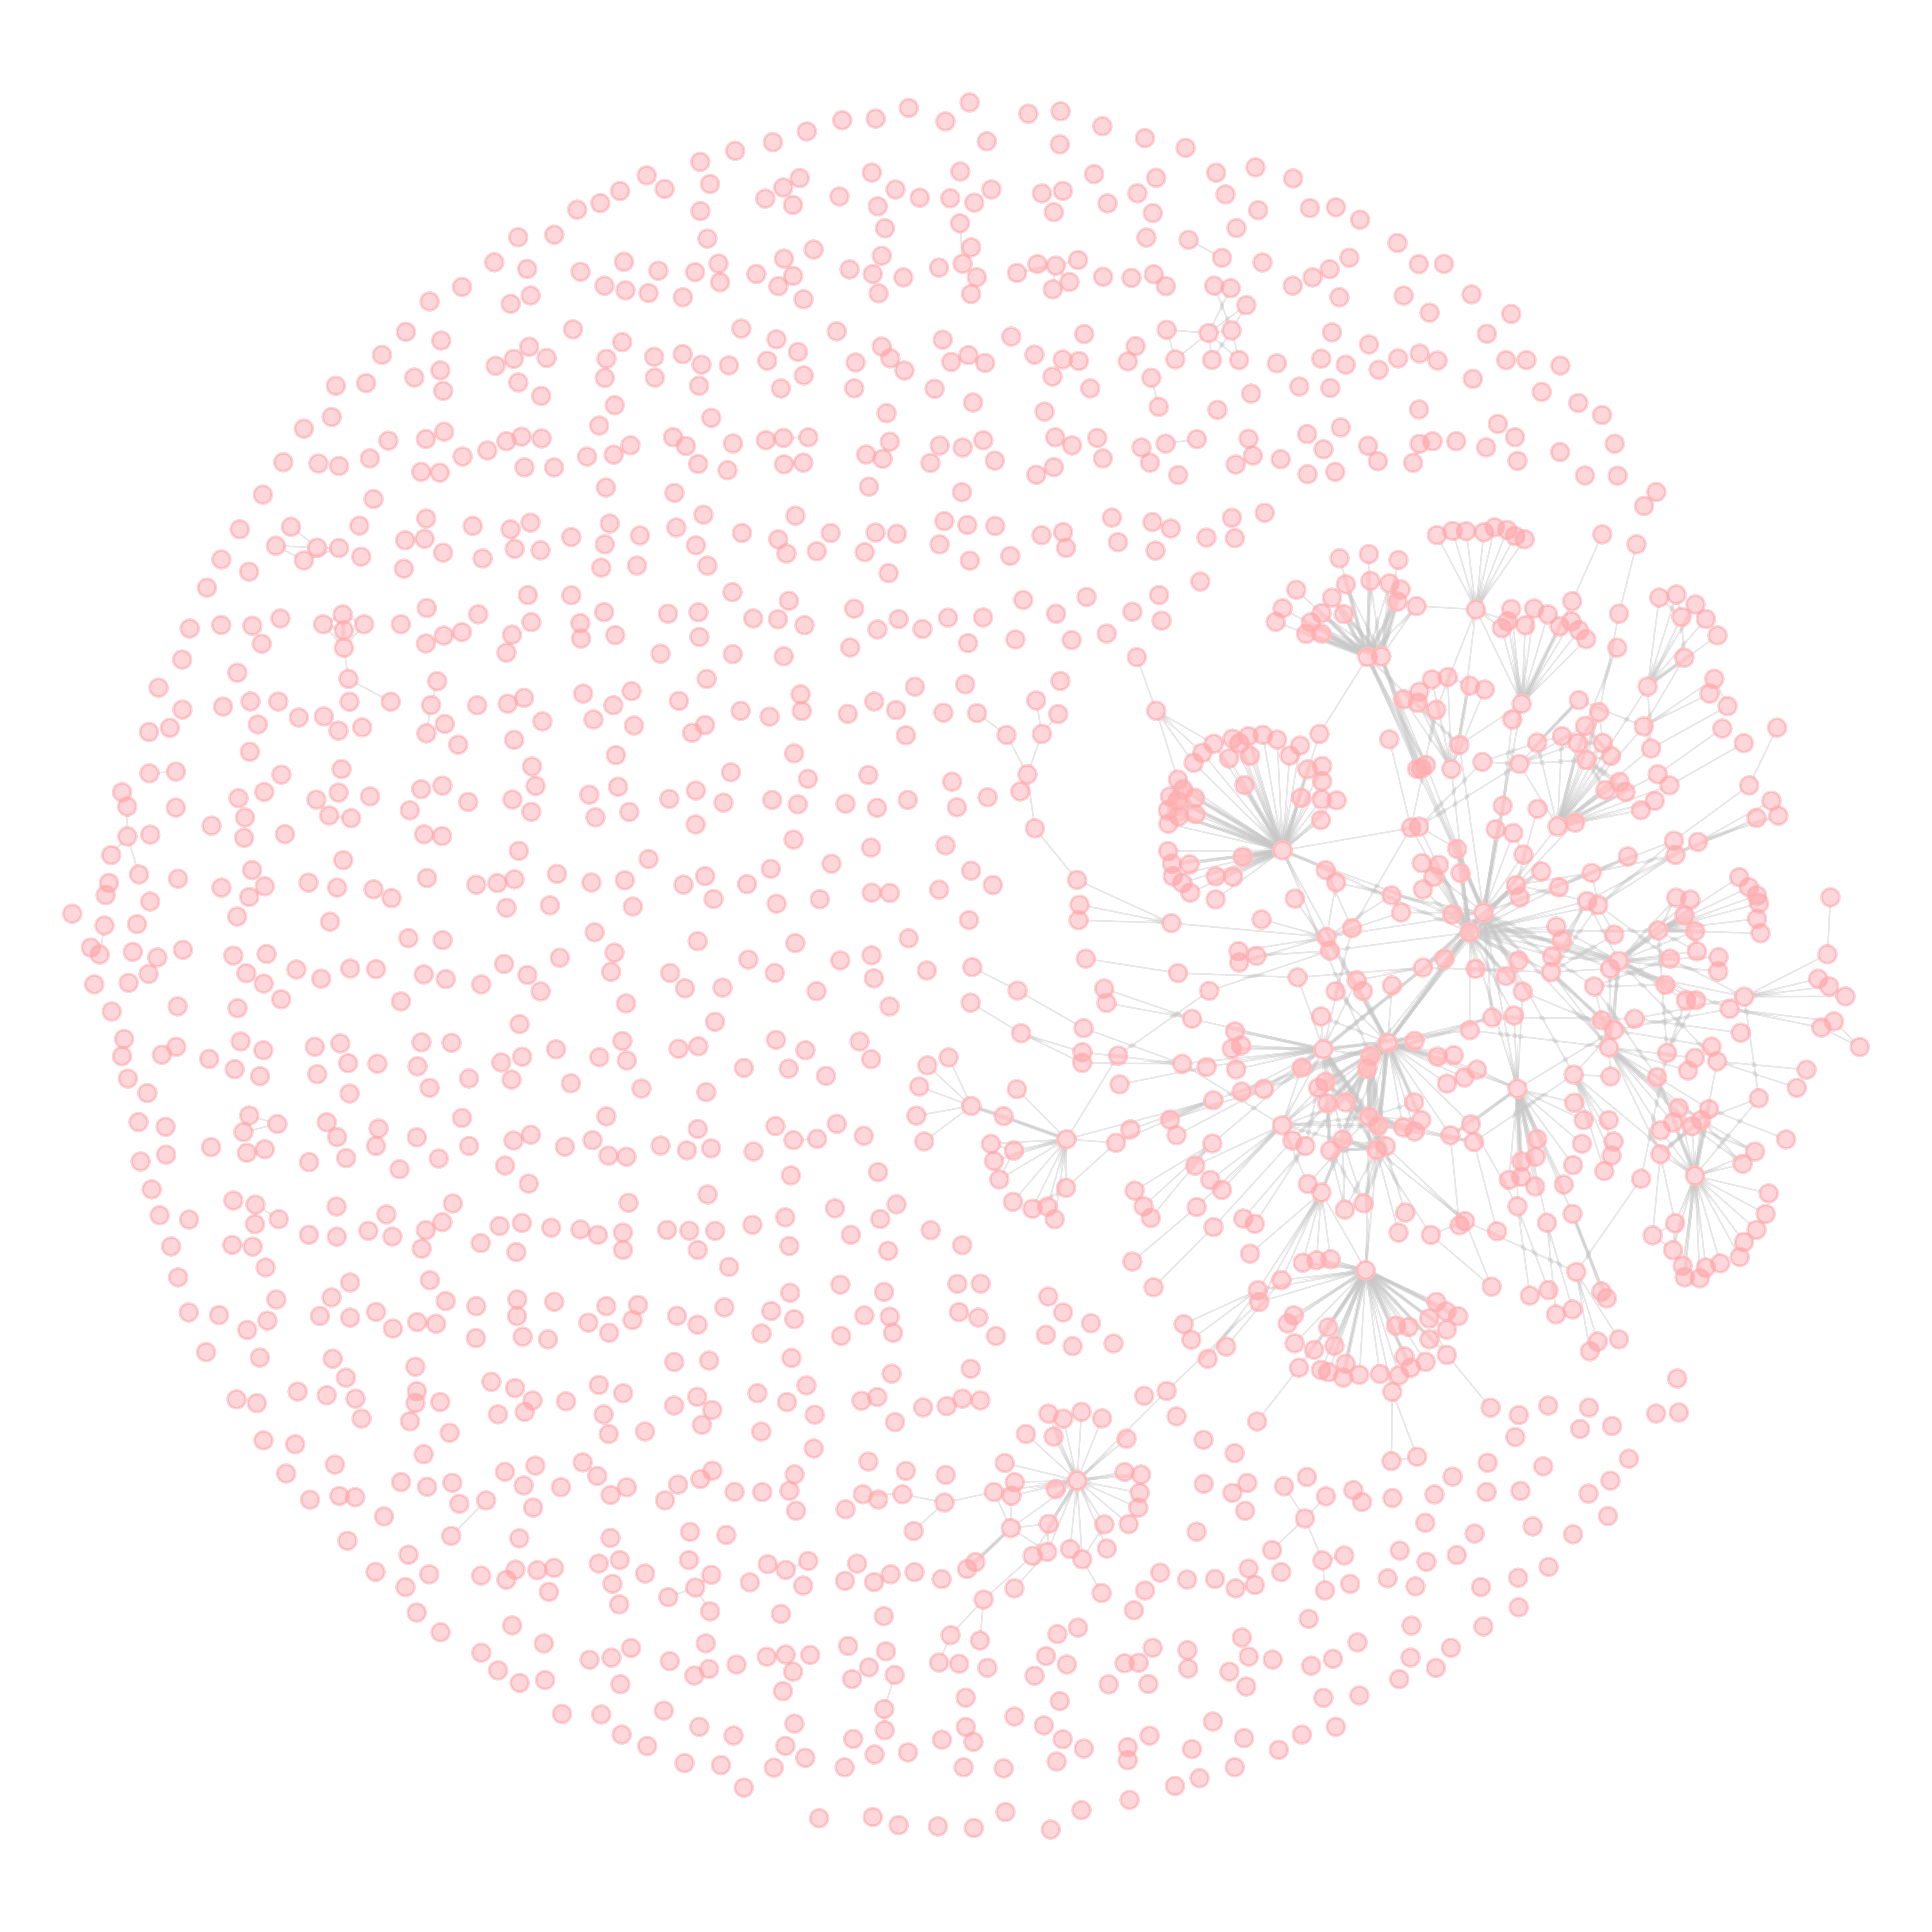
\includegraphics[width=\paperwidth]{graphics/katrinaplot.png}
\end{textblock*}

\begin{textblock*}{100mm}(20mm,0.3\textheight)
\begin{center}
\begin{itemize}
\item[\textcolor{light-gray}{\textbf{1)}}] \textcolor{light-gray}{Overview of Population/Network Processes}
\item[\textcolor{light-gray}{\textbf{2)}}]\textcolor{light-gray}{Examples}
\item[\textbf{3)}] A Model for Dynamic Networks with Population Processes
\item[\textbf{4)}] Empirical Example
\item[\textbf{5)}] Further Reading
\end{itemize}
\end{center}
\end{textblock*}

%----------- Fix name --------------------------------------------------%
\begin{textblock*}{100mm}(4mm,1.02\textheight)

\includegraphics[width=20mm,height=5mm ]{graphics/white.png}
\end{textblock*}

\begin{textblock*}{100mm}(4mm,1.02\textheight)
\emph{\tiny{\darkblue{Zack W Almquist, UMN}}}
\end{textblock*}
%----------- Fix name --------------------------------------------------%
\end{frame}


%----------- frame ----------------------------------------------%
\begin{frame}{} 

\begin{block}{Modeling Dynamic Networks with Populations Dynamics}
\begin{itemize}
\item Empirical motivation
\item Model based motivation
\item Statistical models for networks
\item A statistical model for dynamic networks with population dynamics  
\end{itemize}
\end{block}

\end{frame}
%----------- frame ----------------------------------------------%




%----------- frame ----------------------------------------------%
\begin{frame}{Population Dynamics in Networks}
\begin{columns}
\column{.5\textwidth}

\only<1>{
\begin{block}{Classic Approach}

Treat Networks as fixed populations

\begin{itemize}
\item Organizational Collaboration 
\begin{itemize}
\item Treat every organization as appearing on every day
\end{itemize}
\end{itemize}

\vspace{1.42in}
\end{block}
}
\only<2>{
\begin{block}{Why is This a Problem?}
\begin{itemize}
\item Major problems for realistic models: Population size and composition dynamics
\begin{itemize}
\item Little work in the network methods literature; prior work limited to very stylized cases
\end{itemize}
\item Extreme problem for phenomena like mass convergence in disasters, conversation dynamics, disease spread, etc. 
\end{itemize}
\vspace{.15in}
\end{block}
}
\column{.5\textwidth}
\only<1-2>{
\begin{block}{Org. Collaboration}
\begin{center}
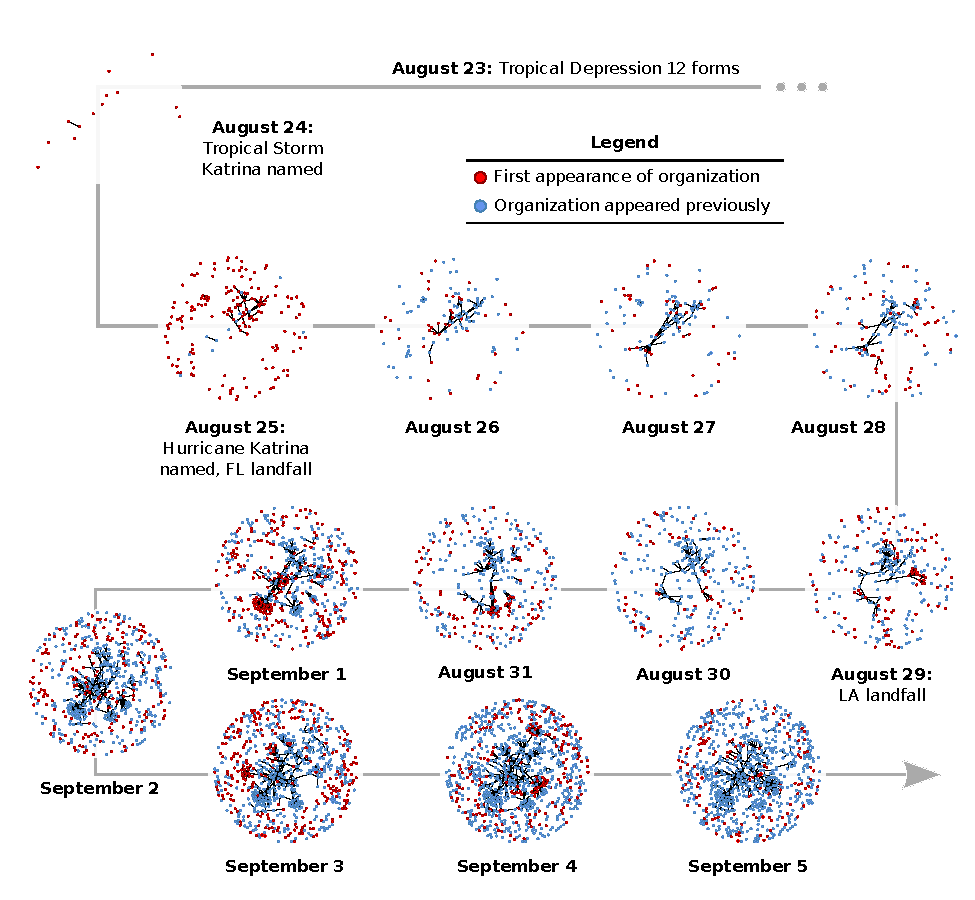
\includegraphics[width=1\linewidth]{graphics/dynamics.pdf}

Figure from: \cite{butts.acton.marcum:2008a}
\end{center}
\end{block}
}
\end{columns}

\end{frame}
%----------- frame ----------------------------------------------%

%----------- frame ----------------------------------------------%
\begin{frame}{What Happens When the Population Process is Ignored?}

\only<1>{
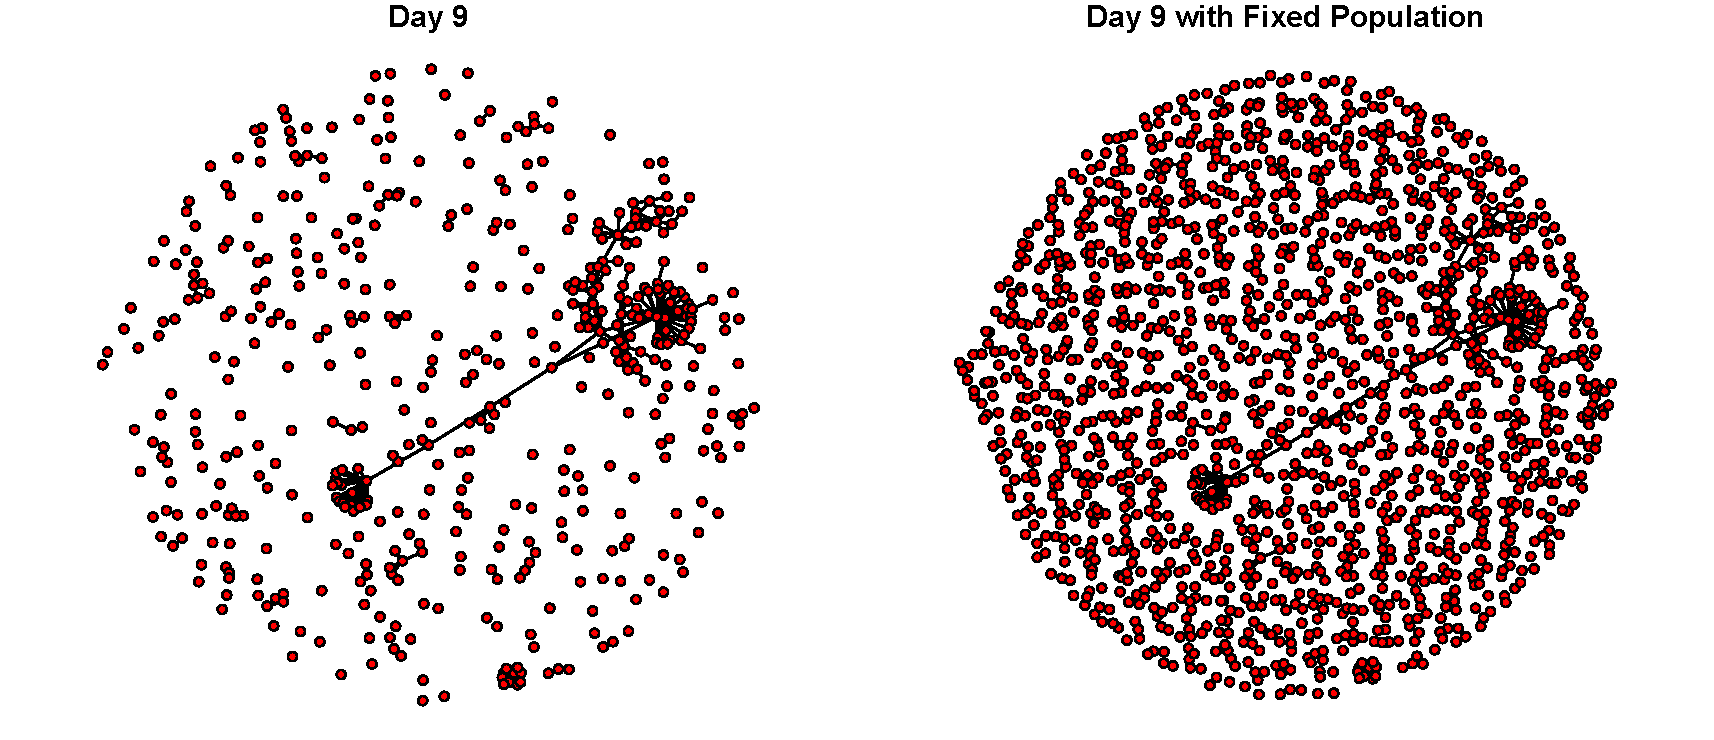
\includegraphics[width=1\linewidth]{graphics/fixedpopplot.pdf}
}
\only<2>{

\begin{textblock*}{80mm}(30mm,.35\textheight)
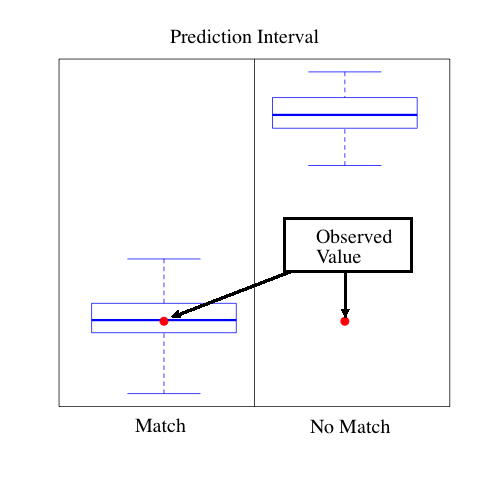
\includegraphics[width=.8\linewidth]{graphics/boxplot.png}
\end{textblock*}

\begin{textblock*}{70mm}(30mm,.13\textheight)
\begin{block}{Aside}
\begin{itemize}
\item Density = $\frac{\textrm{\# Observed Edges}}{\textrm{\# Possible Edges}}$
\item Prediction Interval (boxplot)
\end{itemize}
\end{block}
\end{textblock*}

\begin{textblock*}{100mm}(4mm,1.02\textheight)
\emph{\tiny{\darkblue{Zack W Almquist, UMN}}}
\end{textblock*}

}
\only<3>{
\begin{textblock*}{70mm}(30mm,.2\textheight)
\begin{block}{Naive Population Model}
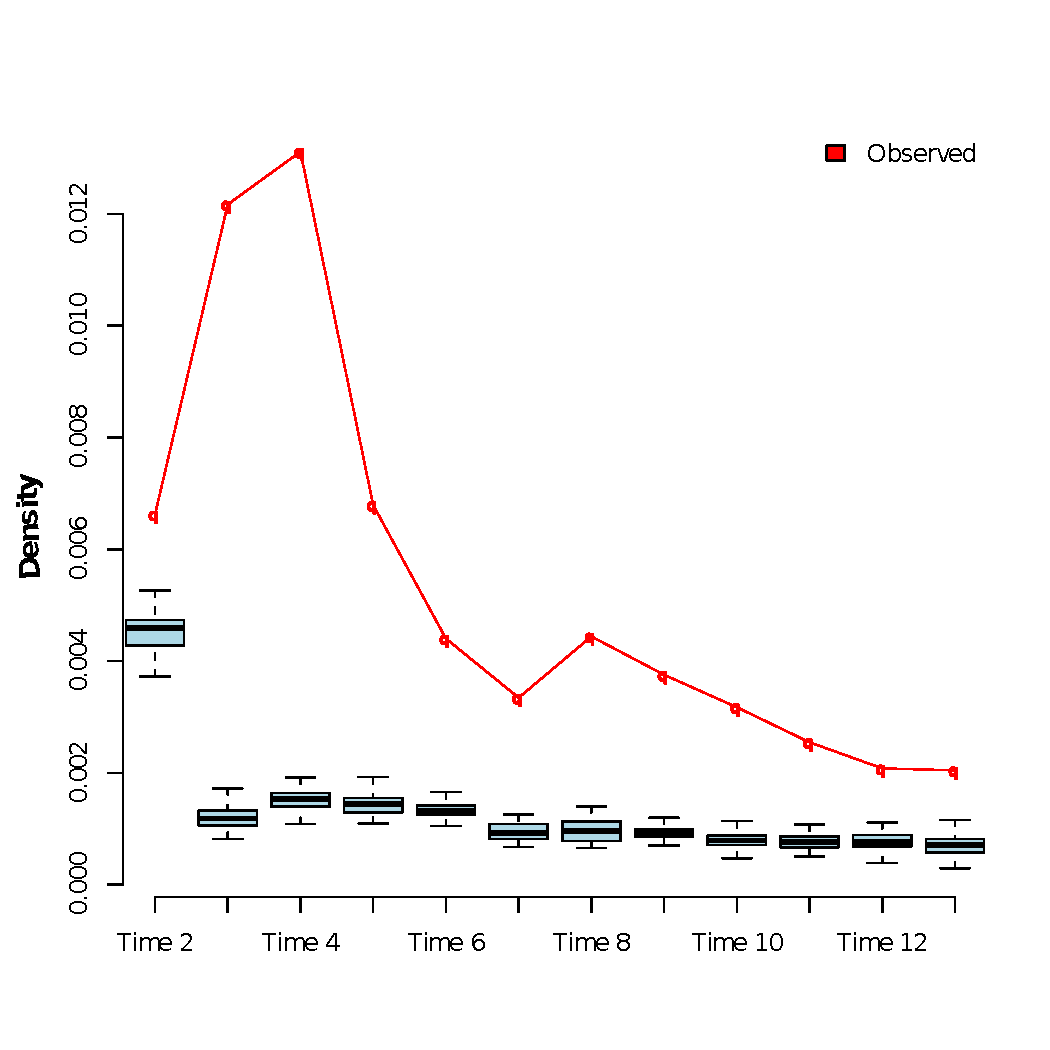
\includegraphics[width=.9\linewidth]{graphics/simpleVertexDensity2}
\end{block}
\end{textblock*}
}
\only<4>{
\begin{textblock*}{70mm}(30mm,.2\textheight)
\begin{block}{Perfect Population: Who Shows Up}
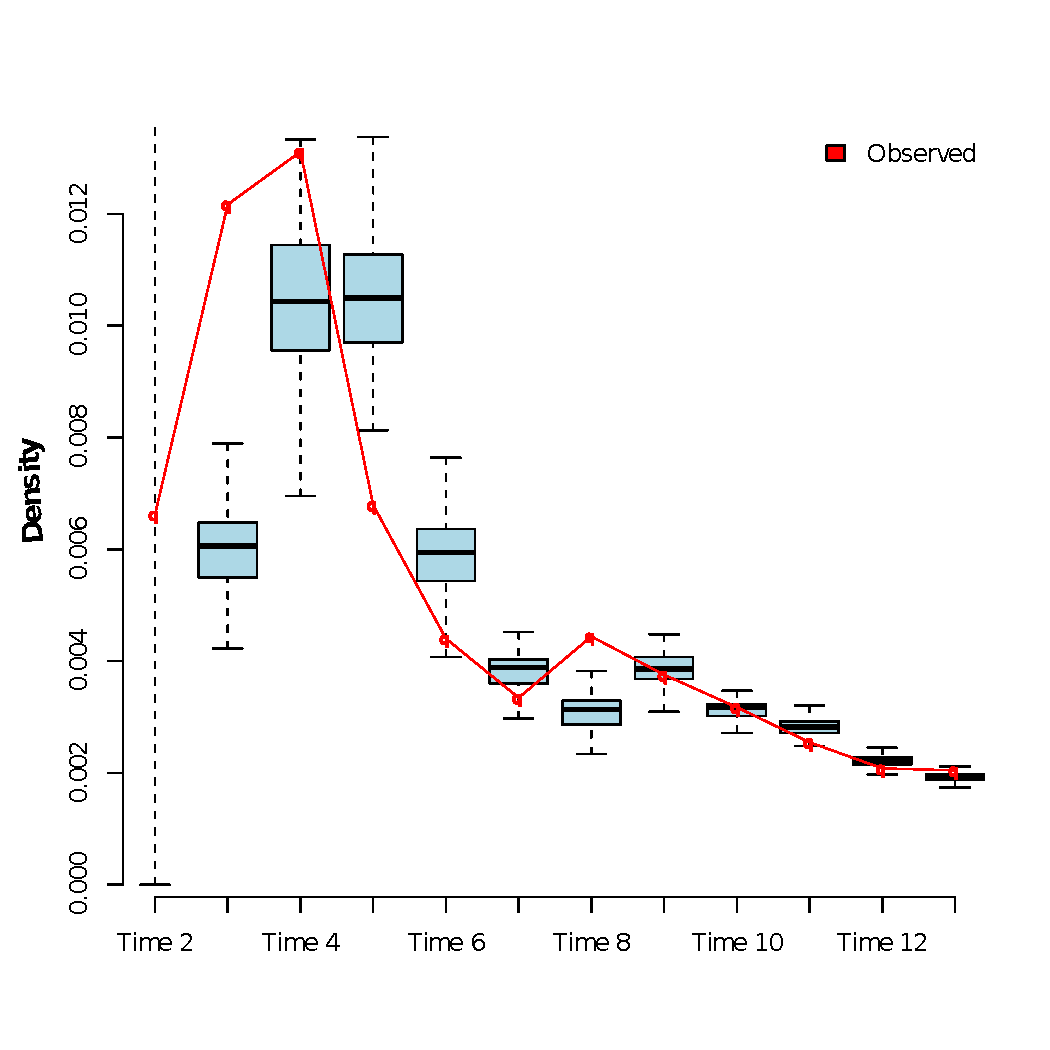
\includegraphics[width=.9\linewidth]{graphics/fixedVertexDensity2} 
\end{block}
\end{textblock*}
}


\end{frame}


%----------- frame ----------------------------------------------%

\begin{frame}{Statistical Models for Social Networks}

%\only<1>{
%\begin{block}{Modeling Dynamic Networks with Vertex Dynamics}
%\begin{itemize}
%\item Mathematical notation for networks
%\item Statistical models for networks (ERGM)
%\item Statistical models for dynamic networks (TERGM)
%\item Statistical models for dynamic networks with population dynamics
%\begin{itemize}
%\item Dynamic Network logistic-Regression (DNR) with Vertex Dynamics 
%\end{itemize}
%\end{itemize}
%\end{block}
%}
\only<1>{
\begin{block}{Network Modeling: Predict the formation and structure of social networks}
\begin{itemize}
\item Many examples
\begin{itemize}
\item Conditional uniform graphs, Bernoulli graphs (baseline models)
\item Holland and Leinhardt's $p_1$ (within dyad dependence)
\item Degree distribution models, growth models, etc.
\end{itemize}
\item Exponential Random Graph Models
\begin{itemize}
\item Draw on theory of statistical exponential families
\item A way of representing and working with new and existing models
\end{itemize}
\end{itemize}
\end{block}
}

\only<2>{

\begin{textblock*}{50mm}(70mm,.2\textheight)
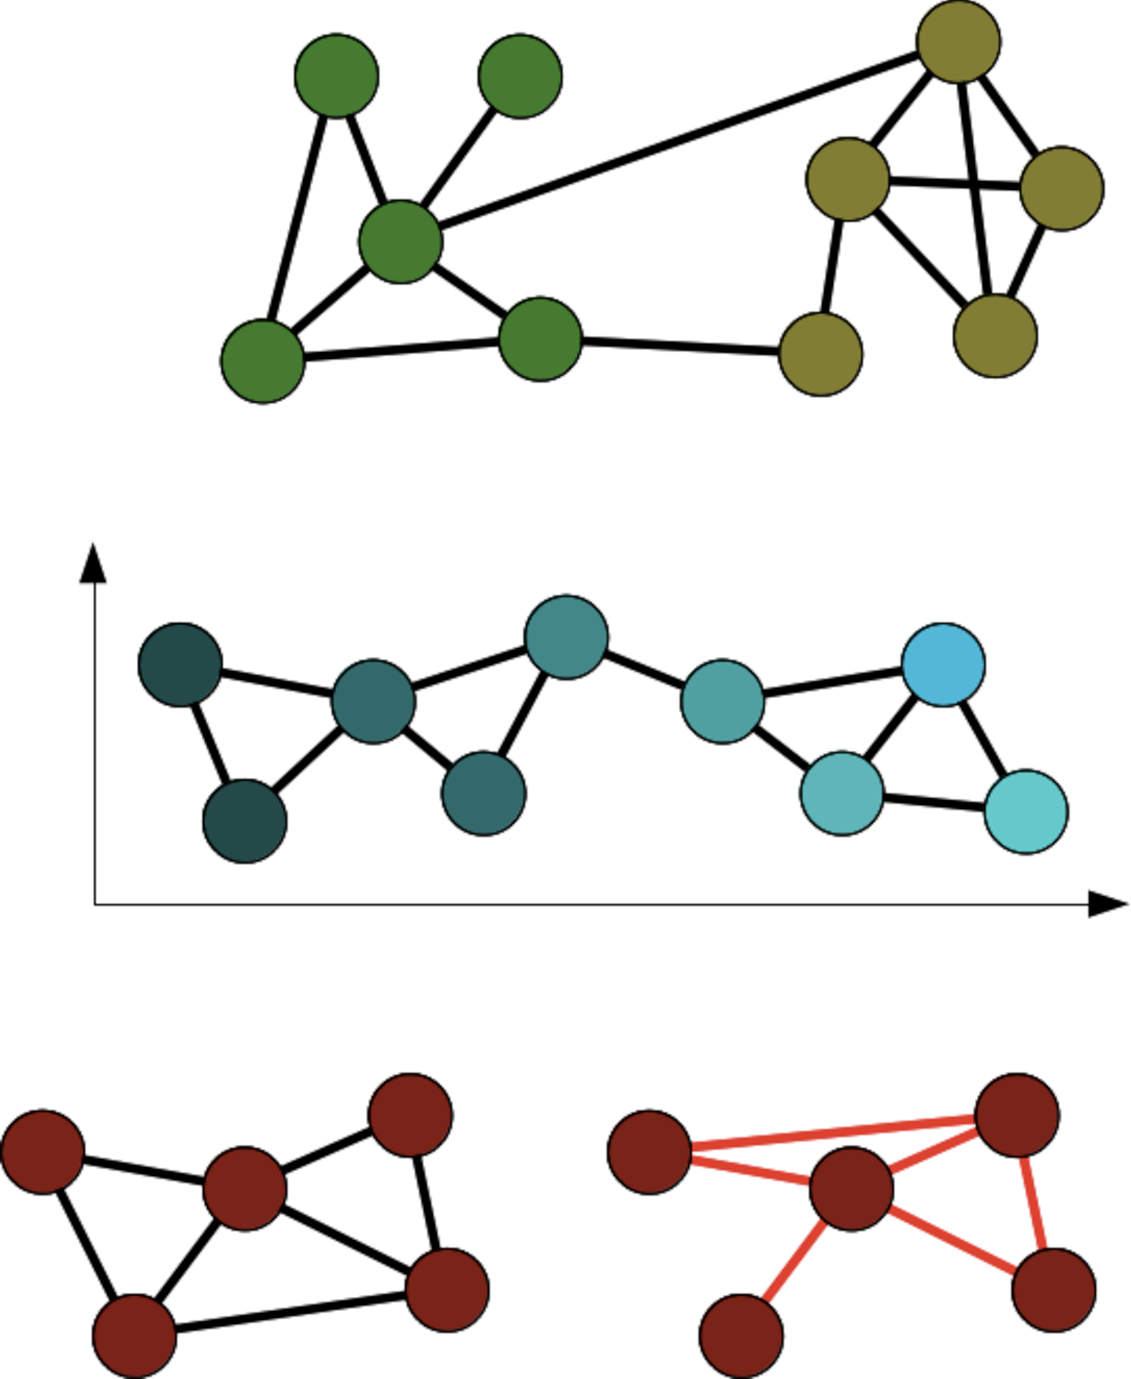
\includegraphics[width=1\linewidth]{graphics/networkexample1.pdf} 
\end{textblock*}

\begin{textblock*}{60mm}(5mm,.25\textheight)
\begin{block}{Initial Intuition: Factors in Tie Formation}
\begin{itemize}
\item All ties are not equally probable 
\begin{itemize}
\item Chance of an $(i,j)$ edge may depend on properties of $i$ and $j$
\item Can also depend on other $(i,j)$ relationships
\end{itemize}
\item Some examples:
\begin{itemize}
\item Homophily
\item Propinquity
\item Multiplexity
\end{itemize}
\end{itemize}
\end{block}
\end{textblock*}
}
\only<3>{
\begin{block}{Exponential Random Graph Model (ERGM)}
\begin{equation*} \label{ergm}
\Pr(G=g \: | \: X ) =\frac{ \exp \left(\theta^T s(g,X) \right) }{{\displaystyle \sum_{g^{'} \in \mathcal{G}}} \exp \left(\theta^T s(g^{'},X) \right)} 
\end{equation*}
\end{block}
}
\only<3>{
\begin{itemize}
\item $G$ is a random network 
\item $g$ belongs to the support, $\mathcal{G}$
\item $\theta$ is a vector of parameters
\item $s(g)$ is a known vector of graph statistics on $g$
\end{itemize}
}
\only<4>{
\begin{textblock*}{50mm}(70mm,.2\textheight)
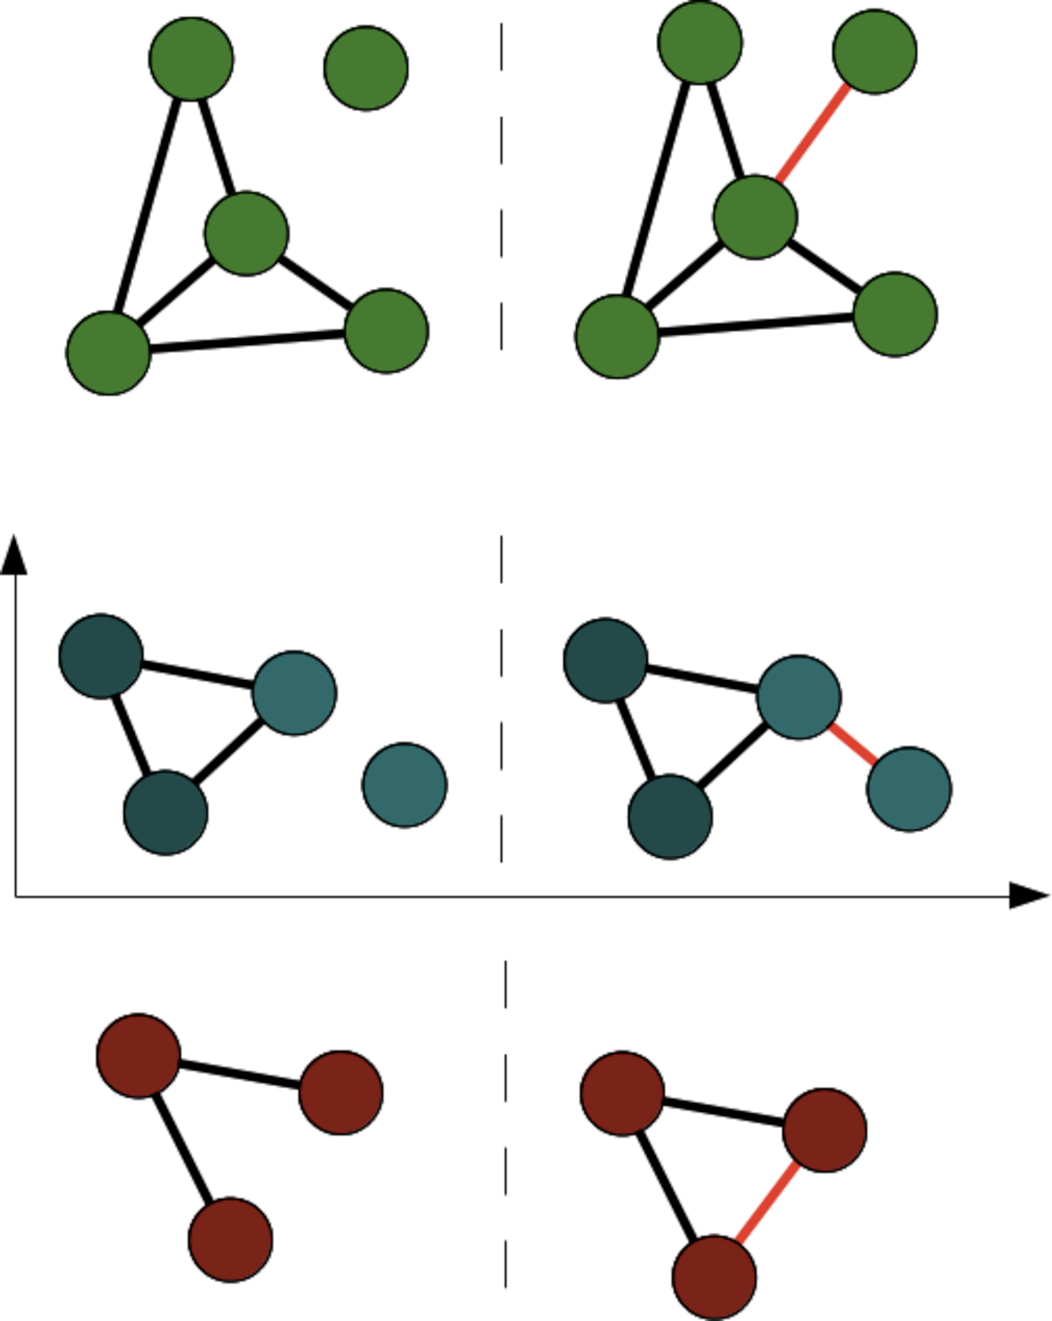
\includegraphics[width=1\linewidth]{graphics/exampleNetwork2.pdf} 
\end{textblock*}

\begin{textblock*}{60mm}(5mm,.25\textheight)
\begin{block}{Initial Intuition: Factors in Tie Formation over Time}
\begin{itemize}
\item All ties are not equally probable 
\begin{itemize}
\item Chance of an $(i,j)$ edge may depend on properties of $i$, $j$ and $t$
\item Can also depend on other $(i,j,t)$ relationships
\end{itemize}
\item Some examples:
\begin{itemize}
\item Homophily
\item Propinquity
\item Triadic/clustering effects
\begin{itemize}
\item Shared partner effects
\end{itemize}
\end{itemize}
\end{itemize}
\end{block}
\end{textblock*}
}
%\only<4>{
%\begin{block}{ERGM (Adjacency Matrix Form)}
%\centering
%$$P_ {\theta}(Y=y) \propto \exp\{ {\theta^T}{s(y})\}$$
%or
%$$P_ \theta(Y=y) = \frac{\exp\{ {\theta^T} {s(y} )\}}
%{c( \theta)},$$
%\end{block}
%where
%\begin{itemize}
%\item $Y$ is a random network on $n$ nodes (a matrix of 0's and 1's)
%\item $\theta$ is a vector of parameters
%\item $s(y)$ is a known vector of graph statistics on $y$
%\end{itemize}
%}
\only<5>{
\begin{block}{Temporal Exponential Random Graph Model (TERGM)}
\begin{align*}
\Pr(G_t =g_t \: | \: G_{t-1},\dots, G_{t-k} ,X) = \frac{ \exp \left(\theta^T s(g_t,G_{t-1},\dots, G_{t-k},X) \right) }{{\displaystyle \sum_{g^{'} \in \mathcal{G}} } \exp \left(\theta^T s(g_t^{'},G_{t-1},\dots, G_{t-k},X) \right)}
\end{align*}
\end{block}
}
\only<5>{
\begin{itemize}
\item $G_t$ is independent of $G_1,\dots,G_{t-2}$ given $G_{t-1}$ \citep{hanneke10} 
\item Arbitrary lags ($G_{t-1},\dots, G_{t-k}$)
\item $g_t$ belongs to the support, $\mathcal{G}$
\item $s$ here is a vector of real-valued sufficient statistics
\item $\theta$ is a vector of parameters  
\item Notice that the denominator is intractable
\end{itemize}
}

%\only<5>{
%\begin{block}{TERGM w/ Vertex Dynamics (Population Dynamics)}
%\begin{align*}
%\Pr(G_t&=g_t \: | \: G_{t-1},\cdots,G_{t-k},X) =\\
%& \Pr(V_t =v_t \: | \: Z_{t-k}, X )\times \\
%&\Pr(Y_t=y_t \: | \: V_{t}, Z_{t-k},X)  \\
%&=\frac{ \exp \left(\psi^T w(v_t,Z_{t-k},X) \right) }{\sum_{v^{'} \in \mathcal{V}} \exp \left(\psi^T w(v_t^{'},Z_{t-k},X) \right)}   \\
%&\times \frac{ \exp \left(\theta^T u(y_t,V_t,Z_{t-k},X) \right) }{\sum_{y^{'} \in \mathcal{Y}} \exp \left(\theta^T u(y_t^{'},V_t,Z_{t-k},X) \right)}, 
%\end{align*}
%\end{block}
%\begin{itemize}
%\item For observations in the support
%\item $Z_{t-k}=(V_{t-1},Y_{t-1}),\cdots, (V_{t-k},Y_{t-k})$
%\end{itemize}
%}
\only<6>{
\begin{center}
\synttree{4}
[{ }
[$\Pr(G_t | G_{t-1},\dots, G_{t-k})$ [\alert{$\Pr(V_t | Z_{t-1},\dots Z_{t-k})\Pr(Y_t|V_t,Z_{t-1},\dots, Z_{t-k})$} [{Dynamic Network logistic-Regression (DNR)}] ] [$\Pr(Y_t|Y_{t-1},\dots, Y_{t-k})$ [\hspace{5mm} Classic DNR] ] ]
]

\begin{textblock*}{100mm}(0mm,.8\textheight)
\small{w/ Vertex Dynamics \citep{almquist12}}
\end{textblock*}

\begin{textblock*}{100mm}(20mm,.25\textheight)
\begin{center}
Temporal Exponential Random Graph Model (TERGM) \\
\small{\cite[e.g.,][]{robbins99,xing07}}
\end{center}
\end{textblock*}
\end{center}

}
\only<7>{
\begin{center}
\synttree{4}
[{ }
[$\Pr(G_t | G_{t-1},\dots, G_{t-k})$ [$\Pr(V_t | Z_{t-1},\dots Z_{t-k})\Pr(Y_t|V_t,Z_{t-1},\dots, Z_{t-k})$ [\alert{Dynamic Network logistic-Regression (DNR)}] ] [$\Pr(Y_t|Y_{t-1},\dots, Y_{t-k})$ [\hspace{5mm} Classic DNR] ] ]
]

\begin{textblock*}{100mm}(0mm,.8\textheight)
\small{ \alert{w/ Vertex Dynamics \citep{almquist12}}}
\end{textblock*}

\begin{textblock*}{100mm}(20mm,.25\textheight)
\begin{center}
Temporal Exponential Random Graph Model (TERGM) \\
\small{\cite[e.g.,][]{robbins99,xing07}}
\end{center}
\end{textblock*}
\end{center}

}

\end{frame}
%----------- frame ----------------------------------------------%





\begin{frame}{\normalsize{How Do We Model Networks and Population Processes Simultaneously?}}

\begin{block}{Key Insight}

\begin{itemize}
\item Comes from separating the \alert{population process} (the vertex set) from the \alert{network process} \dots
\end{itemize}

\end{block}

\end{frame}


\begin{frame}{A Dynamic Network Model with Population Dynamics}
\only<1>{
\begin{block}{Dynamic Network logistic-Regression w/ Vertex Dynamics}
\begin{itemize}
\item Note that this can be recast as a logistic regression problem
\item Formally,
\end{itemize}
\scriptsize{
\begin{align*}
\Pr(V_t\: &|\:Z_{t-1},\dots,Z_{t-k},X) \\ &= \prod_{i=1}^n B\left(\mathbb{I}(v_i \in V_t)\left|\textrm{logit}^{-1} \left(\psi^T w(i,Z_{i-1},\dots,Z_{i-k},X)\right)\right.\right)  \\
\Pr(Y_t\: &|\: V_t, Z_{t-1},\dots,Z_{t-k},X)\\ &= \prod_{(i,j)\in V_t \times V_t}^n B\left(Y_{ij,t}\left|\textrm{logit}^{-1} \left(\theta^T u(i,j,V_t,Z_{i-1},\dots,Z_{i-k},X) \right)\right.\right),\\
\textrm{where } &Z_{t-k} = (Y_{t-k},V_{t-k})
\end{align*}
}
\vspace{.1in}
\end{block}
}
\only<2>{
\begin{block}{Dynamic Network logistic-Regression w/ Vertex Dynamics}
\begin{itemize}
\item Note that this can be recast as a logistic regression problem
\item Formally,
\end{itemize}
%\scriptsize{
\vspace{.1in}
\begin{align*}
%\textrm{logit}\Pr(V_t\: |\:Z_{t-1},\dots,Z_{t-k},&X) =\\
\log\left( \frac{\Pr (\mathbb{I}(V_i \in V_t) = 1)}{ \Pr (\mathbb{I}(V_i \in V_t) = 0)} \right)&= \psi^T w_{i}(Z_{t-1},\dots,Z_{t-k},X) \\ \\
%\textrm{logit}\Pr(Y_t\:|\: V_t, Z_{t-1},\dots,Z_{t-k},&X) = \\
\log\left( \frac{\Pr(Y_{ij,t} = 1)}{\Pr(Y_{ij,t} = 0)} \right)&= \theta^T u_{ij}(V_t,Z_{t-1},\dots,Z_{t-k},X)
\end{align*}
\vspace{.25in}
\end{block}
}


\begin{alertblock}{}
A flexible framework (TERGM subfamily) that readily scales to thousands of vertices/time points
\end{alertblock}

\begin{textblock*}{3in}(20mm,0.42\textheight)

\fbox{%
\begin{minipage}[b][3.3cm][t]{9cm}
\hspace{6.25in}
\end{minipage}}

\end{textblock*}


\end{frame}



%%%%%%%%%%%%%%%%%%%%%%%%%%%%%%%%%
%%%% Model AA
%%%%%%%%%%%%%%%%%%%%%%%%%%%%%%%%%
\subsubsection{Model Adequacy Assessment for DNR w/ Vertex Dynamics} 

\begin{frame}
\frametitle{Model Adequacy Assessment for DNR w/ Vertex Dynamics}


\begin{block}{Model Assessment by Prediction}
\begin{enumerate}[i)]
\item Model Selection

\begin{itemize}
\item e.g., BIC, AIC \dots
\end{itemize}

\item Simulation analysis of graph statistics (a.k.a. Graph Level Indices (GLI); \cite{hunter08})

\begin{itemize}
\item Simulate one-step-ahead prediction for each time point and compare against observed value
\end{itemize}

%\item Examples to Come \dots
\end{enumerate}
\end{block}

\end{frame}

\begin{frame}[t]{Road Map}

\begin{textblock*}{100mm}(20mm,0.3\textheight)
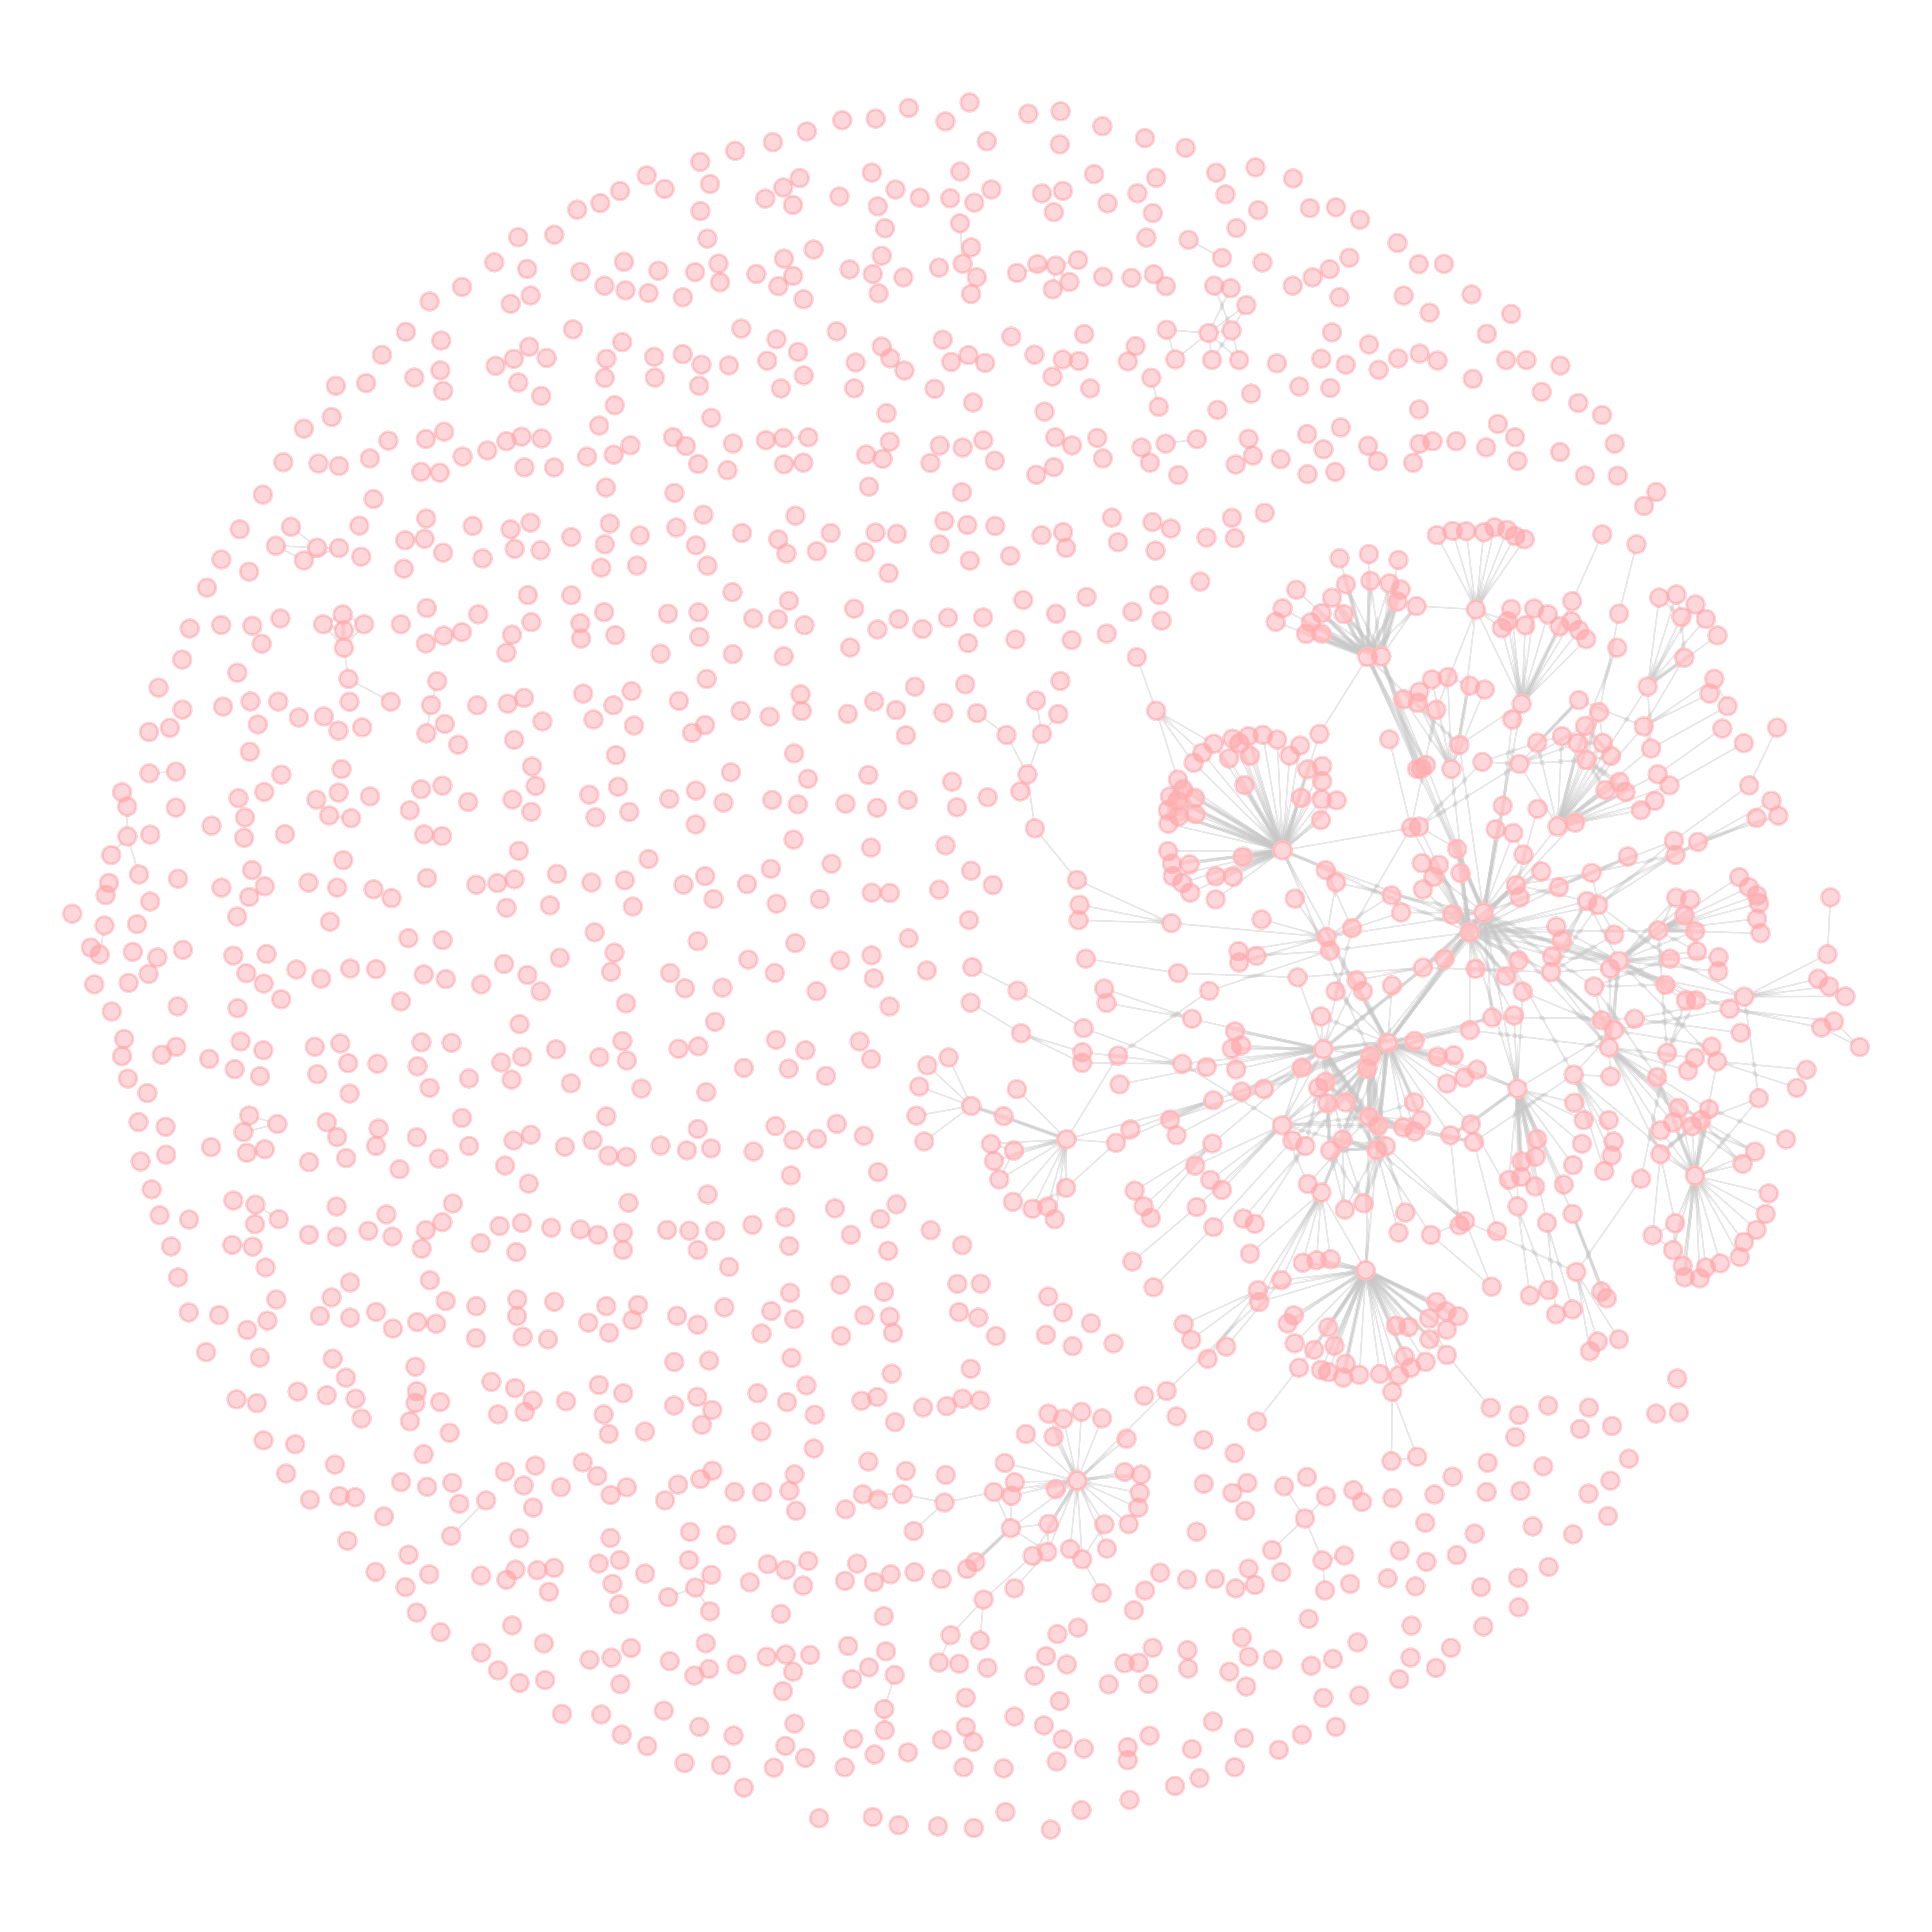
\includegraphics[width=\paperwidth]{graphics/katrinaplot.png}
\end{textblock*}

\begin{textblock*}{100mm}(20mm,0.3\textheight)
\begin{center}
\begin{itemize}
\item[\textcolor{light-gray}{\textbf{1)}}] \textcolor{light-gray}{Overview of Population/Network Processes}
\item[\textcolor{light-gray}{\textbf{2)}}] \textcolor{light-gray}{Examples}
\item[\textcolor{light-gray}{\textbf{3)}}] \textcolor{light-gray}{A Model for Dynamic Networks with Population Processes}
\item[\textbf{4)}] Empirical Example
\item[\textbf{5)}] Further Reading
\end{itemize}
\end{center}
\end{textblock*}

%----------- Fix name --------------------------------------------------%
\begin{textblock*}{100mm}(4mm,1.02\textheight)

\includegraphics[width=20mm,height=5mm ]{graphics/white.png}
\end{textblock*}

\begin{textblock*}{100mm}(4mm,1.02\textheight)
\emph{\tiny{\darkblue{Zack W Almquist, UMN}}}
\end{textblock*}
%----------- Fix name --------------------------------------------------%
\end{frame}


{
\setbeamertemplate{blocks}[rounded][shadow=false]
\begin{frame}{Going to the Beach!}

\begin{center}
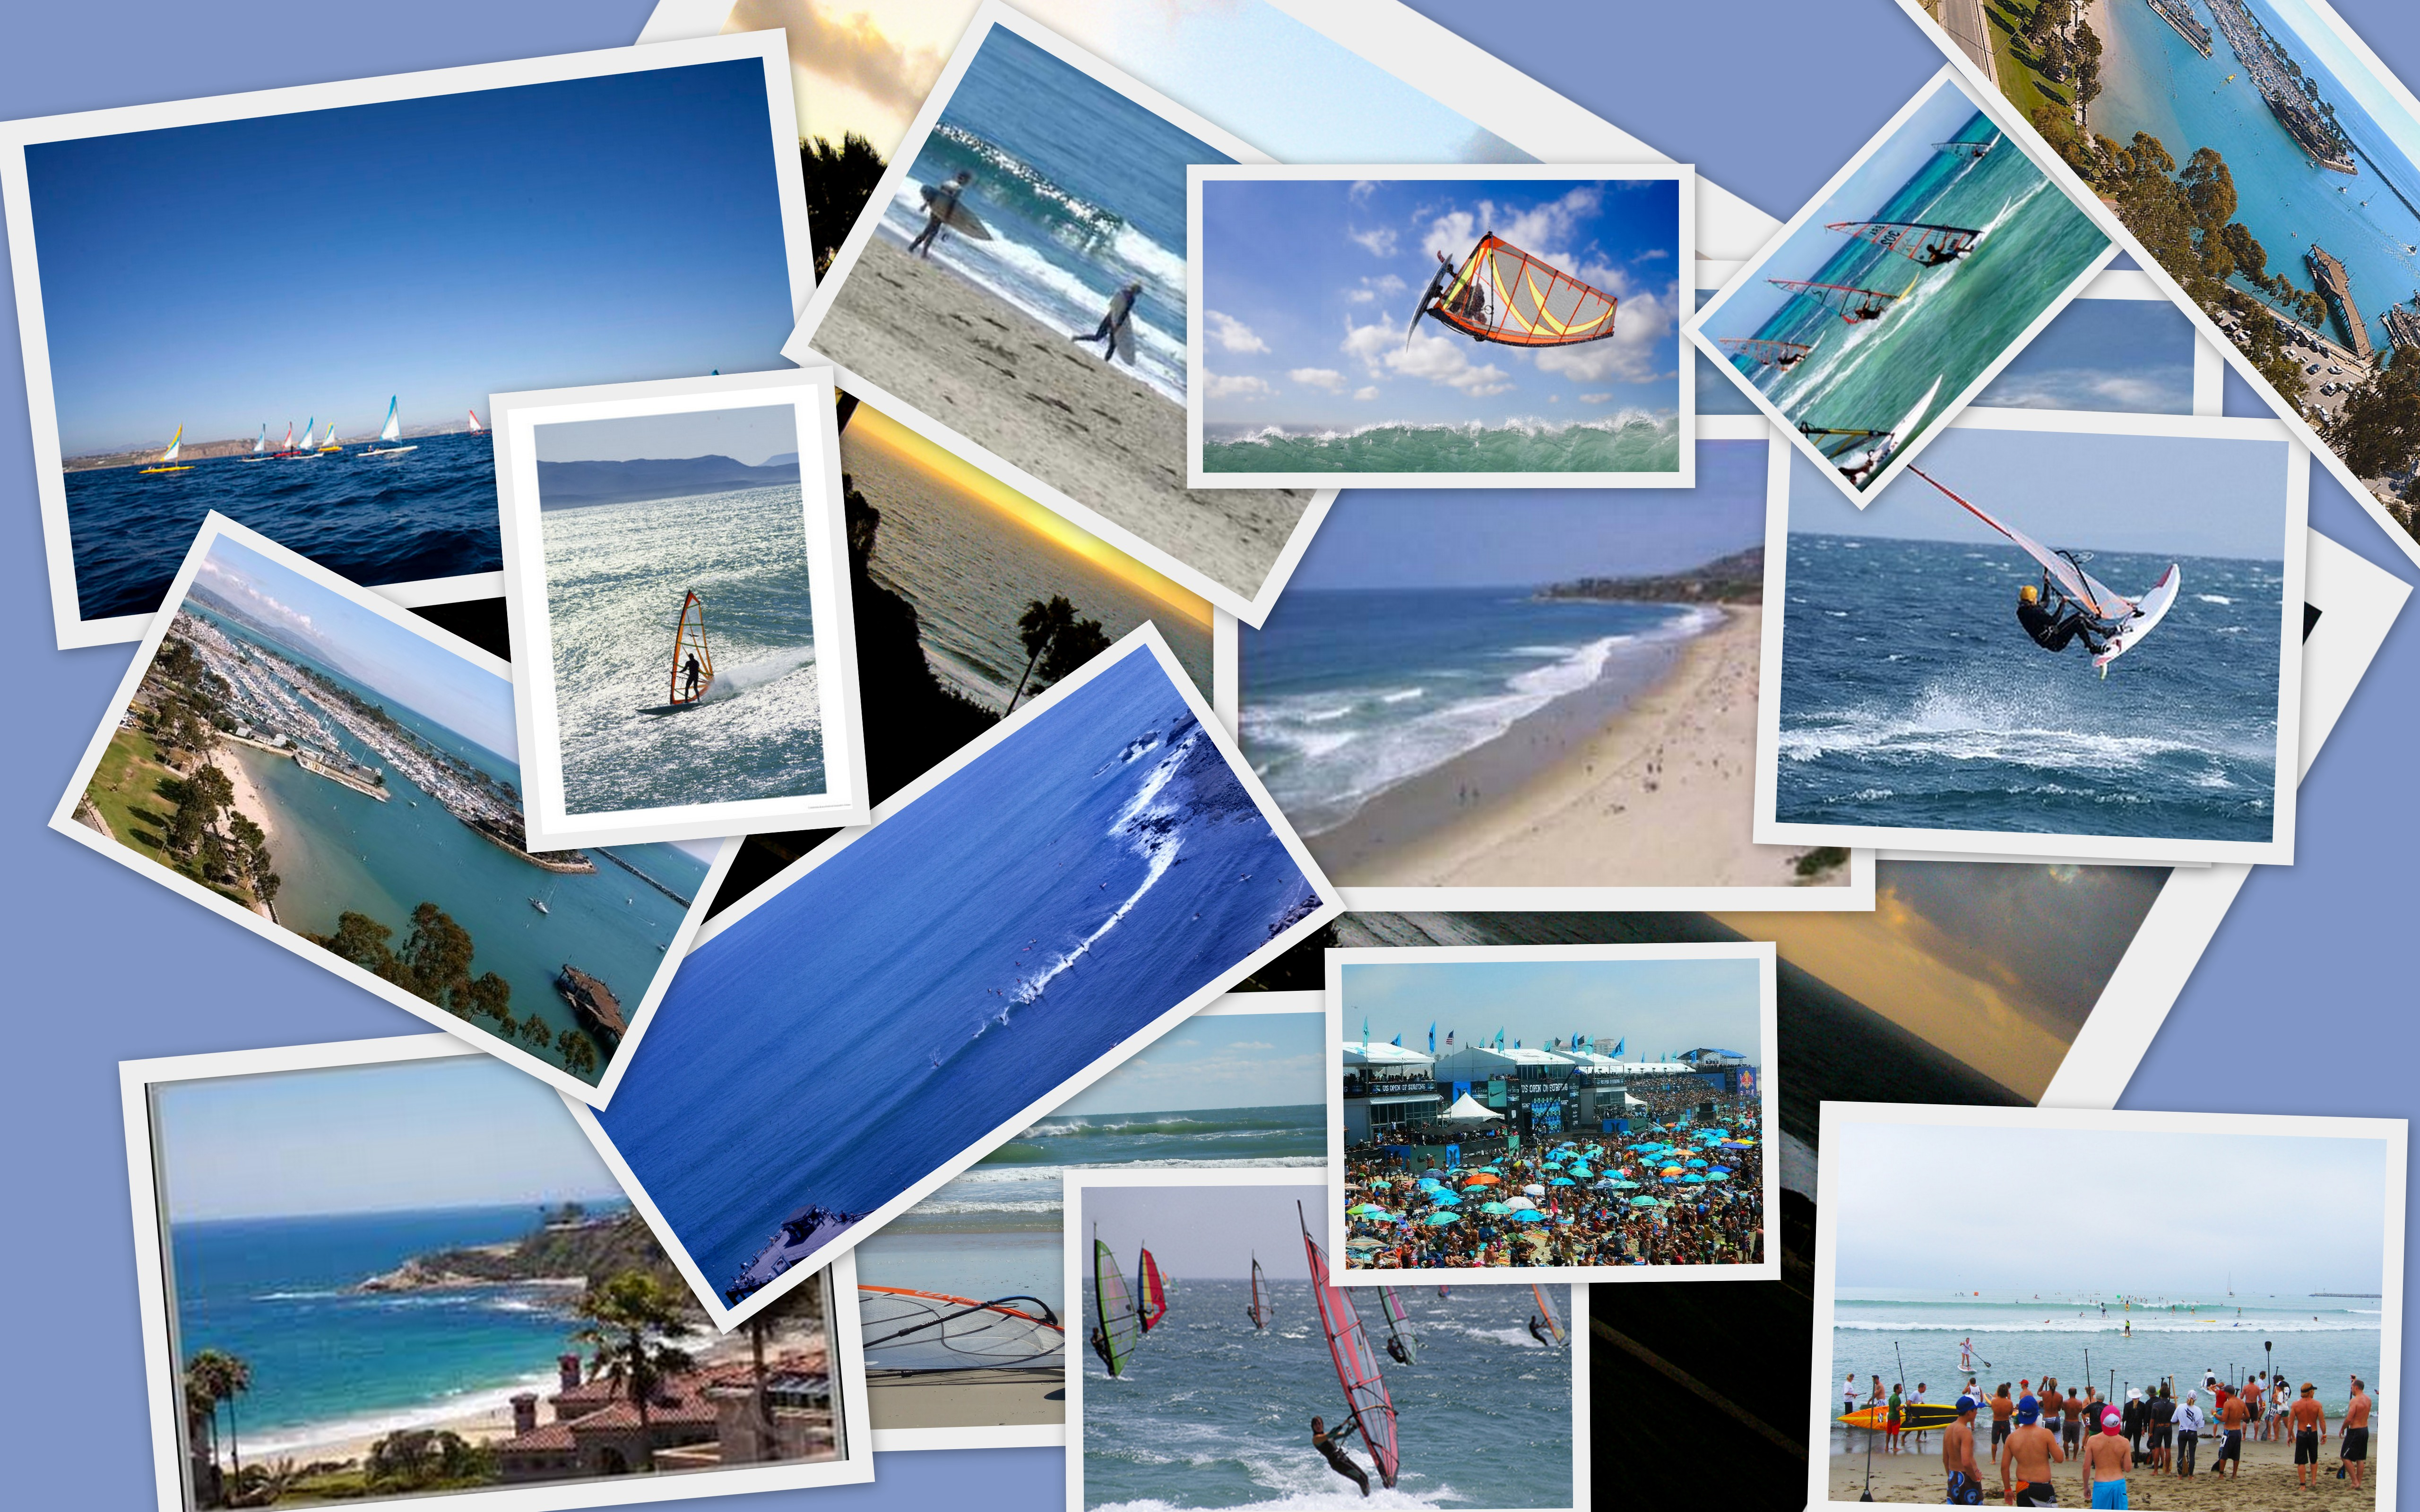
\includegraphics[width=1\linewidth]{graphics/windsurfingPhotos.jpg}
\end{center}

\only<1>{
\begin{textblock*}{90mm}(25mm,.48\textheight)

\includegraphics[width=1\linewidth,height=1cm]{graphics/bgtitle.pdf}
\end{textblock*}
\begin{textblock*}{100mm}(30mm,.5\textheight)
\textbf{\Huge{Going to the Beach!}}
\end{textblock*}
}
\only<2>{
\begin{textblock*}{30mm}(50mm,.35\textheight)
\begin{block}{Lin Freeman}
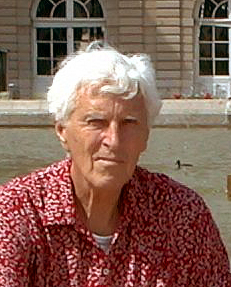
\includegraphics[width=1\linewidth]{graphics/freeman.jpg}
\end{block}
\end{textblock*}
}

\only<3>{
\begin{textblock*}{60mm}(40mm,.45\textheight)
\begin{block}{}
Collected a \alert{dynamically evolving network} of interpersonal communication among individuals congregating on a beach in SoCal observed over a one-month period \citep{freeman88}, but only analyzed \alert{cross-sectional case}
\end{block}
\end{textblock*}
}

\end{frame}
}

{
\setbeamertemplate{blocks}[rounded][shadow=false]
\begin{frame}{The Data: Social Relationships on the Beach}

\begin{center}
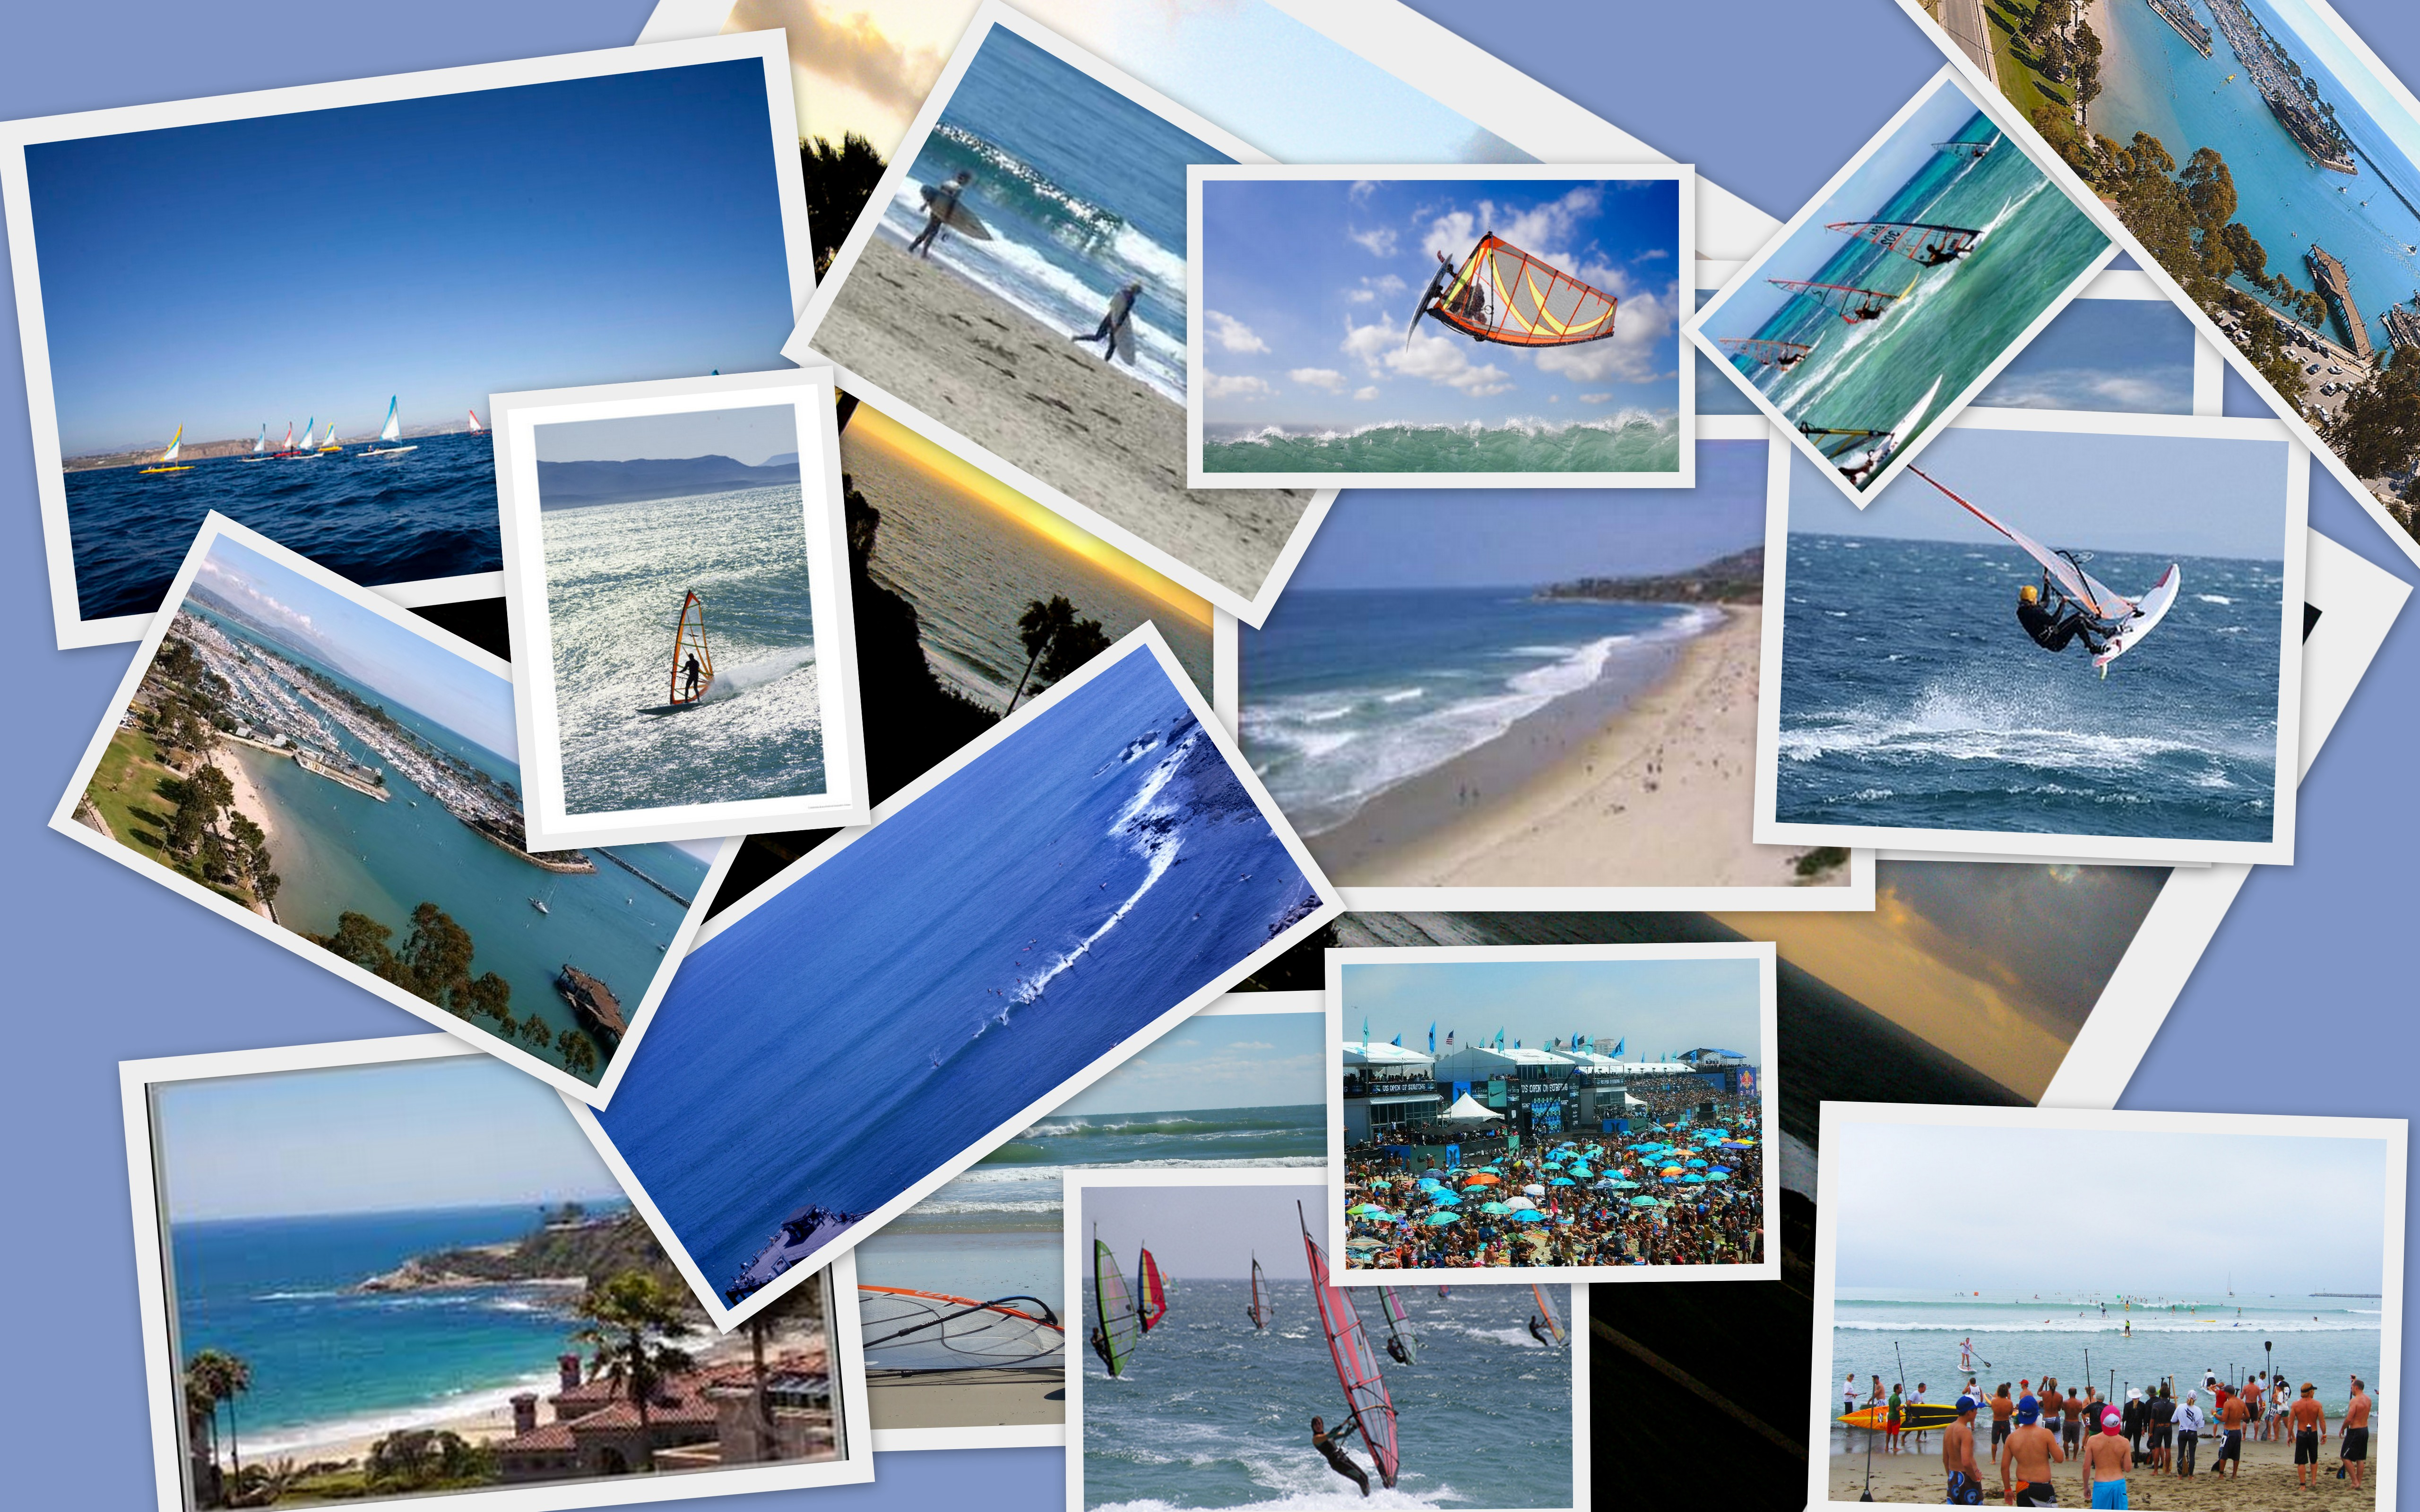
\includegraphics[width=1\linewidth]{graphics/windsurfingPhotos.jpg}
\end{center}

\only<1>{
\begin{textblock*}{90mm}(20mm,.28\textheight)
\begin{block}{}
\small
\begin{itemize}
\item Originally collected to represent informal group dynamics in a natural setting
\item Collected to examine people's ability to perceive and recall patterns of social alliance and separation
\item Lin Freeman et al. (1988) settled on studying windsurfers on a beach in Southern California during the fall of 1986
\begin{itemize}
\item The authors had all been participant observers and windsurfers at the beach for several years
\item Developed a ``sense" of the windsurfing community
\item Knew the people involved well enough to be sure that they would cooperate in the systematic collection of data
\end{itemize}
\end{itemize}
\end{block}
\end{textblock*}
}
\only<2>{
\begin{textblock*}{90mm}(20mm,.15\textheight)
\begin{block}{}
Windsurfing began at the beach (Dana Point) in 1977
\end{block}

\begin{block}{}
\centering
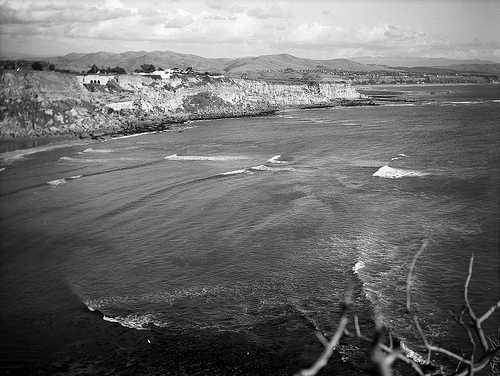
\includegraphics[width=.7\linewidth]{graphics/dana1970.jpg}
\end{block} 

\end{textblock*}
}
\only<3>{
\begin{textblock*}{90mm}(20mm,.15\textheight)
\begin{block}{}
 Started slow, but gradually, as more people got into the sport, a group of ``\death{regulars}" was established
\end{block}

\begin{block}{}
\centering
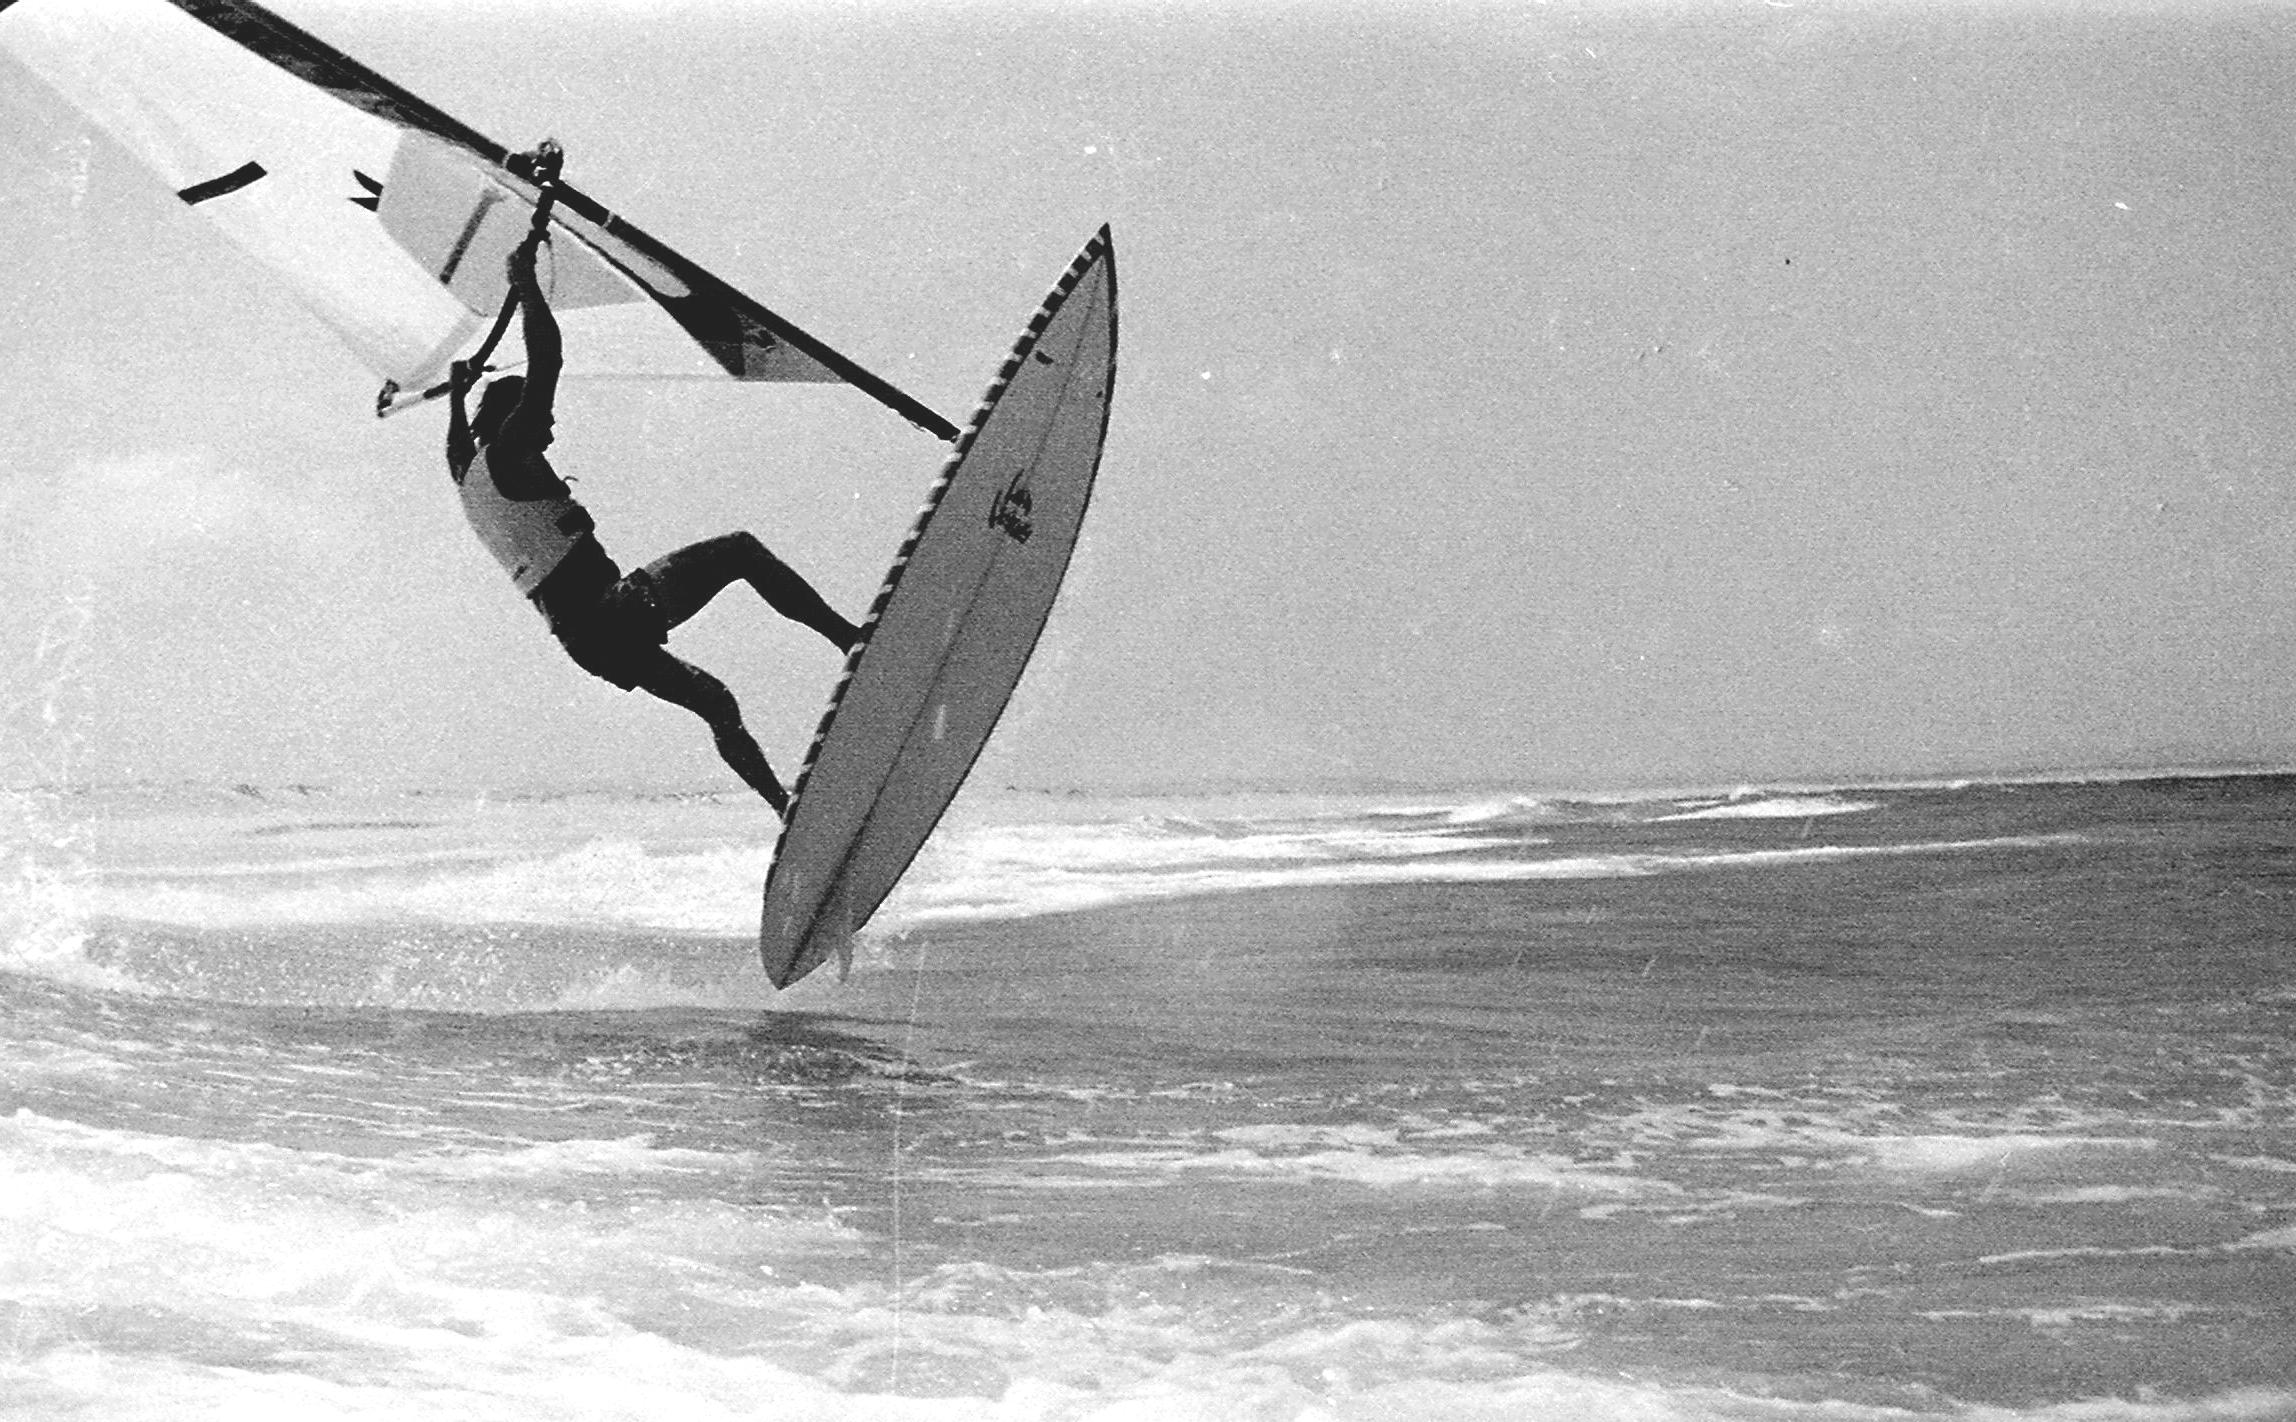
\includegraphics[width=.8\linewidth]{graphics/windsurfer1970.jpg}
\end{block}

\end{textblock*}
}
\only<4>{
\begin{textblock*}{90mm}(20mm,.15\textheight)
\begin{block}{}
These people spent time together and almost totally avoided interacting with other beach users who were not windsurfers
\end{block}

\begin{block}{}
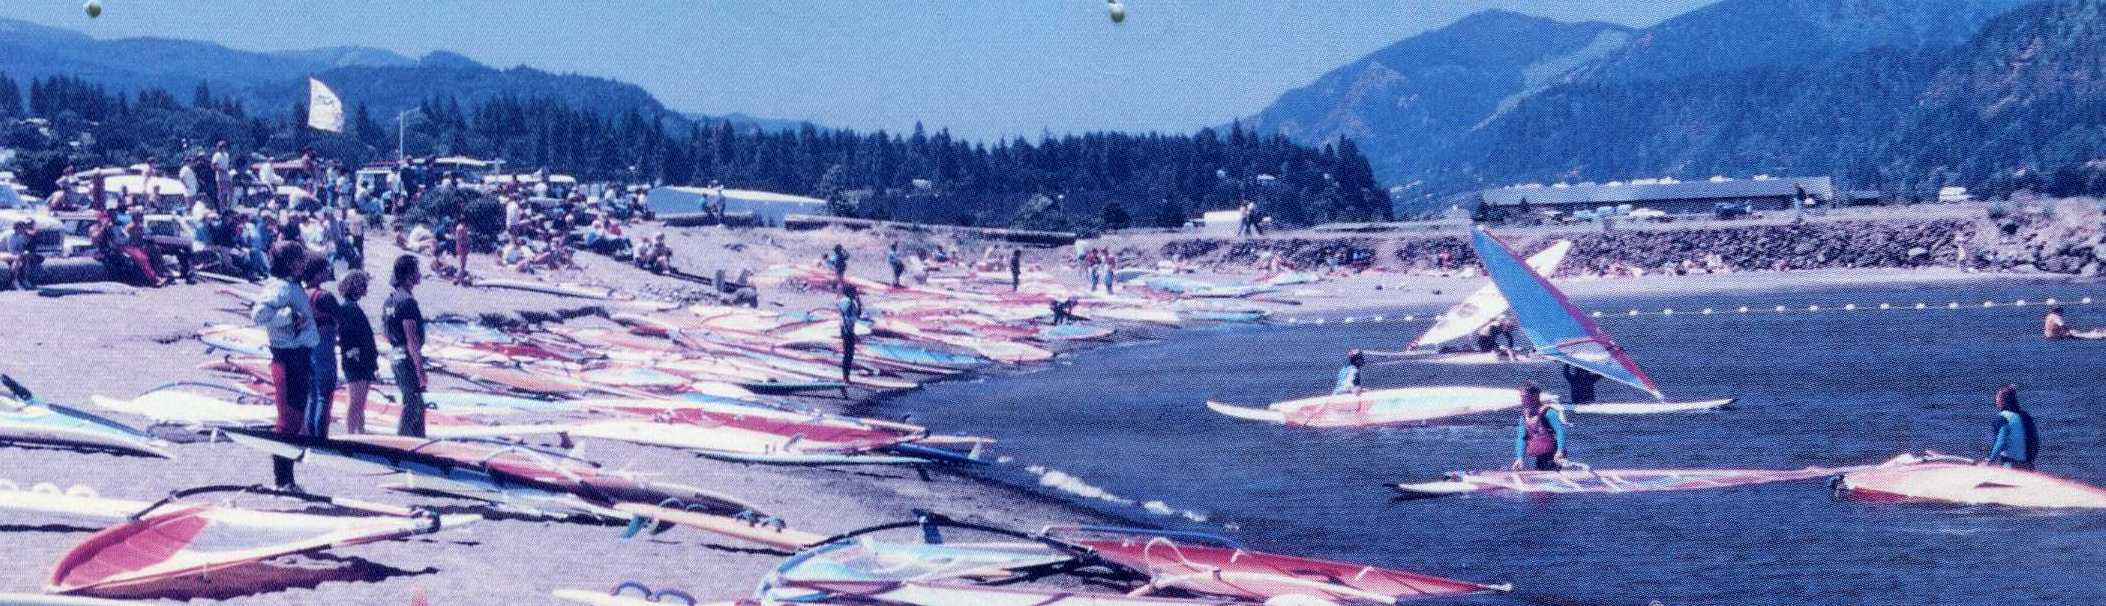
\includegraphics[width=1\linewidth]{graphics/windsurfersOnAbeach.jpg}
\end{block}

\end{textblock*}
}
\only<4>{
\begin{textblock*}{90mm}(20mm,.15\textheight)
\begin{block}{}
This produced insulated group dynamics and a ``community" bound together by a common activity
\end{block}

\begin{block}{}
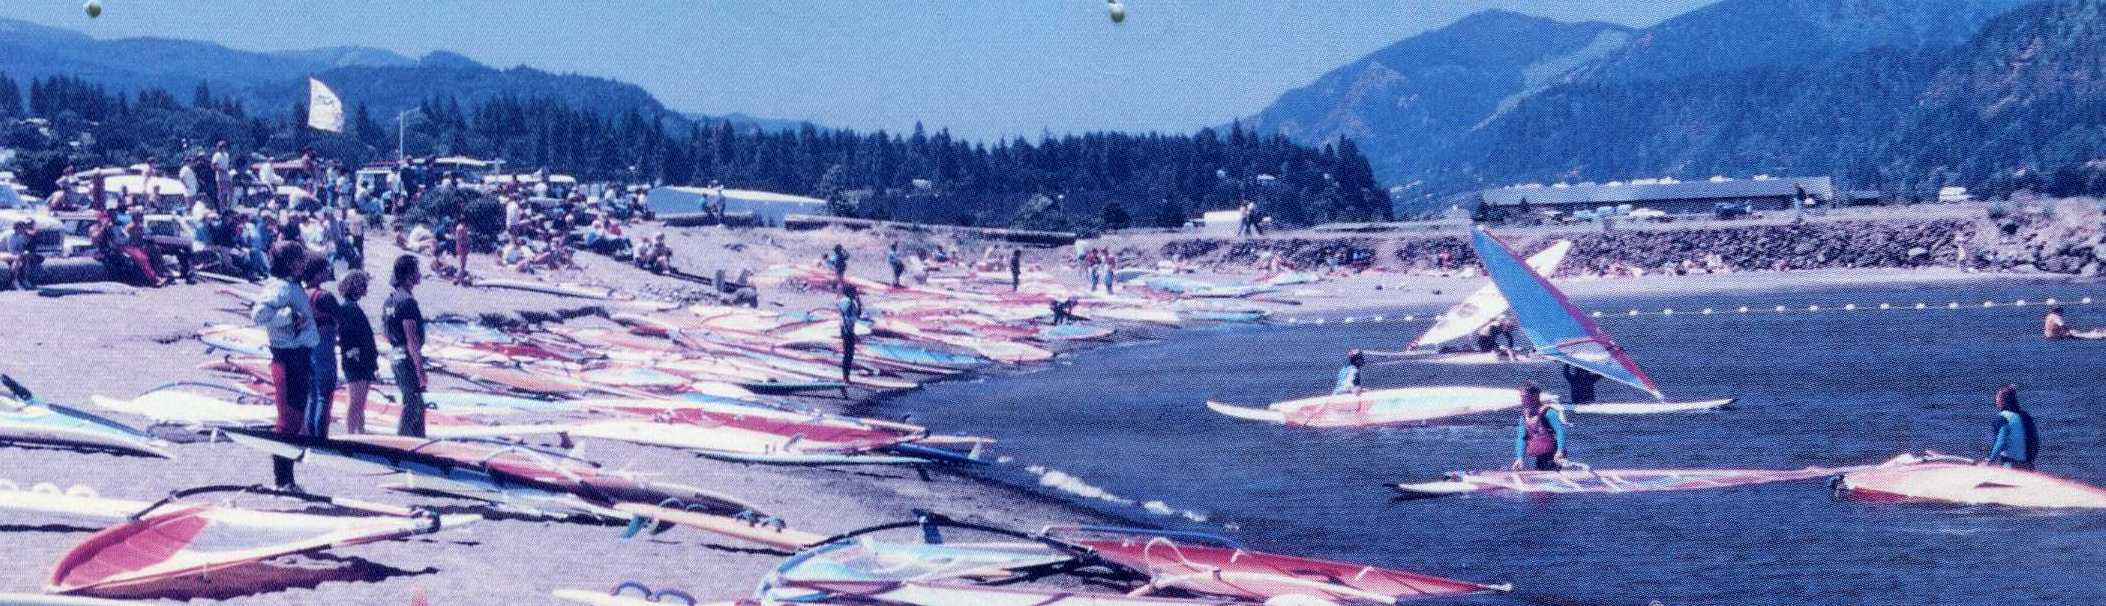
\includegraphics[width=1\linewidth]{graphics/windsurfersOnAbeach.jpg}
\end{block}

\end{textblock*}
}
\only<5>{
\begin{textblock*}{90mm}(20mm,.15\textheight)
\begin{block}{}
By  1983, stable  membership  of  about  25  to  30 (\death{Group1})
\end{block}

\begin{block}{}
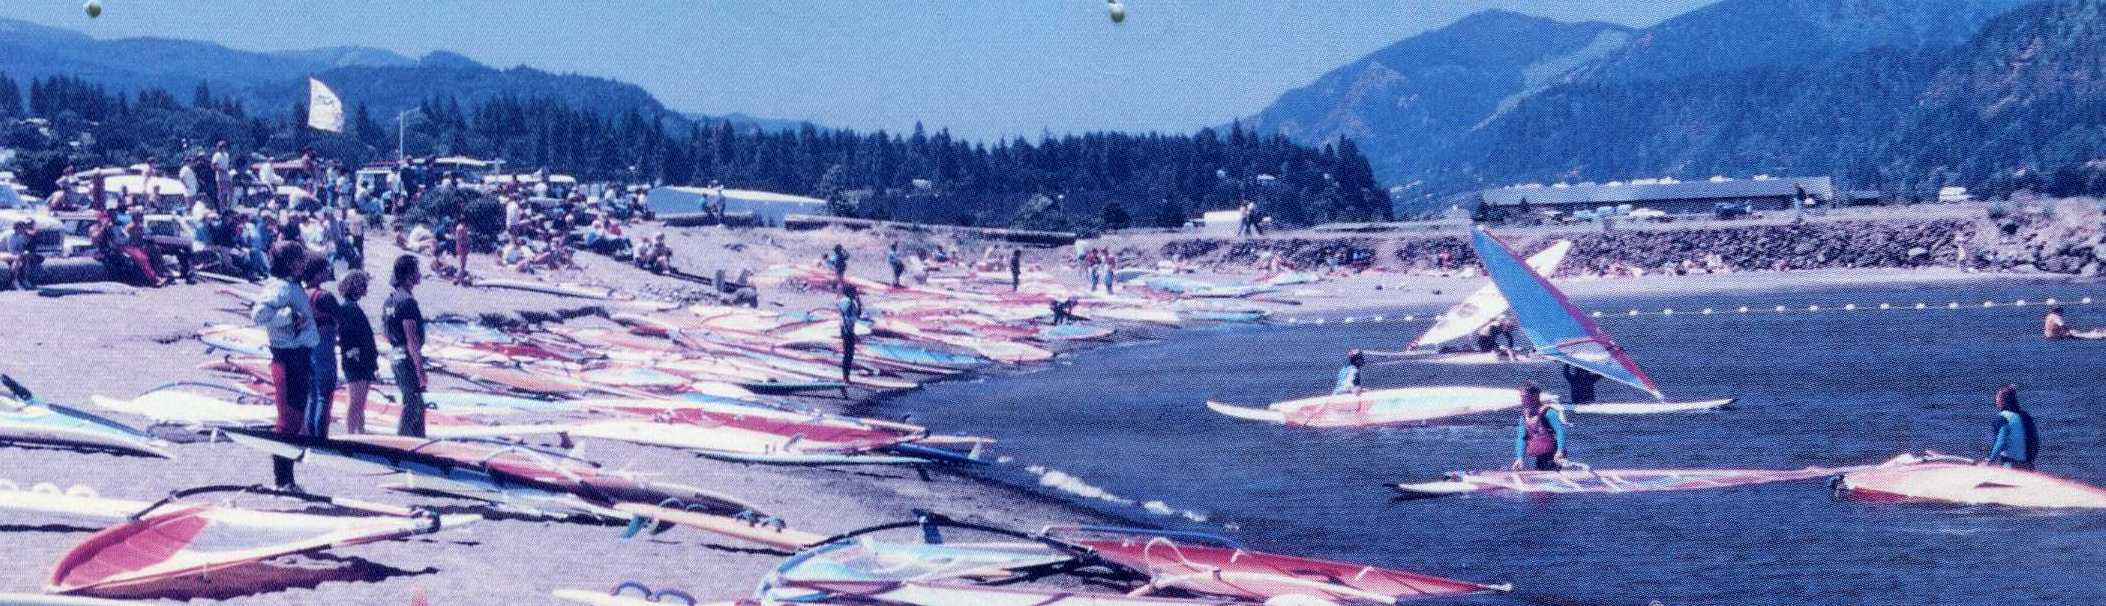
\includegraphics[width=1\linewidth]{graphics/windsurfersOnAbeach.jpg}
\end{block}

\end{textblock*}
}
\only<6>{
\begin{textblock*}{90mm}(20mm,.15\textheight)
\begin{block}{}
That same  year,  windsurfing  experienced  an  upsurge of  interest and beginners  took  it  up  in  increasing  numbers. The  established  windsurfers began to  refuse  to  welcome  new  windsurfers
\end{block}

\begin{block}{}
\centering
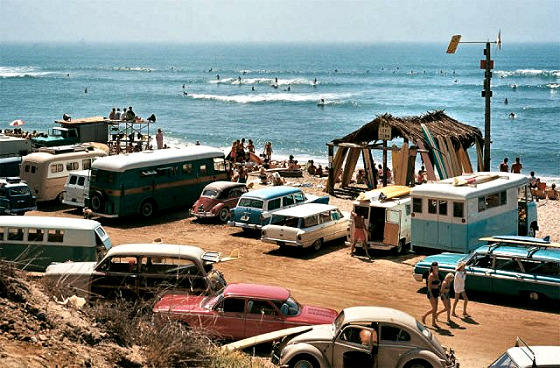
\includegraphics[width=.8\linewidth]{graphics/malibubeach2.jpg}
\end{block}


\end{textblock*}
}
\only<7>{
\begin{textblock*}{90mm}(20mm,.15\textheight)
\begin{block}{}
At  first,  the  new  wave  of  beginners  were  social  isolates. Then,  gradually,  as their  numbers  grew,  these  newcomers  began  to  drift  together  to  form  a  second  informal  group (\death{Group2})
\end{block}

\begin{block}{}
\centering
\includegraphics[width=.75\linewidth]{graphics/mapLinFreeman.png}

\tiny
``Figure  1 shows where  people  (and  their  sails)  were  located  on  the  beach  at  noon  on  27 September  and illustrates  this [two groups]  separation" \citep{freeman88}
\end{block}

\end{textblock*}
}
\only<8>{
\begin{textblock*}{90mm}(20mm,.15\textheight)
\begin{block}{}
Members  of  each  group  seemed,  to  some  degree,  to  limit  their  interaction  to  fellow group  members
\end{block}

\begin{block}{}
\centering
\includegraphics[width=.75\linewidth]{graphics/mapLinFreeman2.png}

\tiny
``Figure  1 shows where  people  (and  their  sails)  were  located  on  the  beach  at  noon  on  27 September  and illustrates  this [two groups]  separation" \citep{freeman88}
\end{block}
\end{textblock*}
}




\end{frame}
}

{
\setbeamertemplate{blocks}[rounded][shadow=false]

\begin{frame}{The Data: Social Relationships on the Beach}
\setbeamercovered{transparent}

\begin{center}
\includegraphics[width=1\linewidth]{graphics/windsurfingPhotos.jpg}
\end{center}

\begin{textblock*}{90mm}(15mm,.3\textheight)
\begin{block}{Net Result}
\begin{itemize}
\item<1> 30 days of network dynamics and population dynamics
\item<2>  Informal group interaction over a month
\item<3> 95 different individuals (ranging from 3 to 37)
\item<4>{ 4 Ethnographically defined classifications

\begin{itemize}
\item Group1 (the old-timers)
\item Group2 (the young-turks)
\item Regulars (Group1 \& 2 $+$ indiv. not app in Group1 or 2)
\item Irregulars
\end{itemize}
}
\end{itemize}
\end{block}
\end{textblock*}
\end{frame}
}


\begin{frame}{}
\begin{block}{Application of Dynamic Network logistic-Regression}
\begin{itemize}
\item Note that this is the first time this data set has been analyzed in a dynamic way
\item \alert{DNR with Vertex Dynamics} allows one to ask interesting questions about group dynamics from observational data
\item \alert{DNR with Vertex Dynamics} allows one to examine the interplay between network dynamics and population dynamics
\end{itemize}
\end{block}
\end{frame}

\begin{frame}{Mech. of Dynamic Interpersonal Communication}
\begin{block}{}
\begin{itemize}
\item[1)] Population Process Model: What Influences Who Shows Up?
\item[2)] Network Model: What Influences Who Talks to Whom?
\end{itemize}
\end{block}
\end{frame}

\begin{frame}{Mech. of Dynamic Interpersonal Communication}
\begin{block}{Population Process Model: What Influences Who Shows Up?}
\begin{itemize}
\item<1-5> Regularity effect (dummy for Regulars and Group1)
\item<1-5> Inertial effect (lag term)
\only<2>{
\begin{itemize}
\item  e.g., \citet{corten10}
\end{itemize}
}
\item<1-5> Triadic effect (3-cycle or triadic closure)
\only<3>{
\begin{itemize}
\item  e.g., \citet{faust10,wasserman94}
\end{itemize}
}
\item<1-5> Seasonality (dummy for each day of the week)
\only<4>{
\begin{itemize}
\item  e.g., \citet{butts09,baker:ajs:1984}
\end{itemize}
}
\end{itemize}
\end{block}
\end{frame}



\begin{frame}{Mech. of Dynamic Interpersonal Communication}
\begin{block}{Network Model: What Influences Who Talks to Whom?}
\begin{itemize}
\item<1-8> Regularity of beach use (Mixing terms for regulars)
\only<2>{
\begin{itemize}
\item  e.g., \citet{mcpherson01}
\end{itemize}
\centering
\includegraphics[width=.3\linewidth]{graphics/regularity.pdf}
}
\item<1-8> Indiv. propensity effects for regularly occurring indiv. (dummy) 

\only<3>{
\centering
\includegraphics[width=.5\linewidth]{graphics/indivProp.pdf}
}
\item<1-8> Contagious participation ($\log(n_t)$)

\only<4>{
\centering
\includegraphics[width=.5\linewidth]{graphics/contPart.pdf}
}

\item<1-8> Inertial network effects (lag term)

\only<5>{
\centering
\includegraphics[width=.5\linewidth]{graphics/intertia.pdf}
}
\item<1-8> Embeddedness (log of 9-cycle effect)
\only<6>{
\begin{itemize}
\item  e.g., \citet{granovetter85}
\end{itemize}
\centering
\includegraphics[width=.3\linewidth]{graphics/ninecycle.pdf}
}
\item<1-8> Seasonality (dummy for each day of the week)
\only<7>{
%\begin{itemize}
%\item  \citep[e.g.,][]{butts09,baker:ajs:1984}
%\end{itemize}
%\centering
\includegraphics[width=.5\linewidth]{graphics/seasonalExample.pdf}
}
\end{itemize}
\end{block}

\end{frame}




\begin{frame}{}
\begin{block}{}
\centering
Model Selection and Assessment 
\end{block}

\end{frame}



%%%%%%%%%%
%% vertex model
%%%%%%%%%%
\begin{frame}{Population Process Model}
\begin{center}
{
\input tables/vertex1.tex
}
\end{center}
\end{frame}

%%%%%%%%%%
%% vertex model
%%%%%%%%%%

%%%%%%%%%%
%% edge model
%%%%%%%%%%


\begin{frame}{Network Model}
\begin{center}
\footnotesize{
\input tables/edge1.tex
}
\end{center}
\end{frame}


\begin{frame}{Model Adequacy Checking}
\begin{table}[ht]
\begin{center}
\begin{tabular}{l|c}
 \multicolumn{2}{c}{\textbf{GLI One-Step Prediction Simulation Count ($\alpha \leq 0.95$)}} \\
  \hline
GLI & Fraction Correct\\
  \hline
Network Size & 26/28 \\ 
  Density & 28/28 \\ 
  Mean Degree & 28/28 \\ 
  Degree Centralization & 20/28\\ 
  Krackhardt Connectedness & 28/28 \\ 
  Triad Census: 0 & 28/28 \\ 
  Triad Census: 1 & 27/28 \\ 
  Triad Census: 2 & 28/28 \\ 
  Triad Census: 3 & 28/28\\ 
   \hline
\end{tabular}
\caption{Check of whether the $\alpha \leq 0.95$ simulation interval contains a given GLI. Total possible correct is 28.}\label{tbl:count}
\end{center}
\end{table}
\end{frame}

\begin{frame}{}
\begin{block}{Results}
\begin{itemize}
\item[1)] Population Process Model
\item[2)] Dynamic Network Model
\end{itemize}
\end{block}

\end{frame}

\begin{frame}{Results: Population Process Model}

\begin{center}
\footnotesize{
\input tables/vertex.tex
}
\end{center}

\only<2>{
\begin{textblock*}{60mm}(32mm,0.49\textheight)
\begin{alertblock}{} 
\small
\begin{itemize}
\item Being  in the ``regular" category $\uparrow$ likelihood~of appearance 
\item Being in Group 1 $\uparrow$ likelihood of appearing
\end{itemize}
\end{alertblock}
\end{textblock*}
}
\only<3>{
\begin{textblock*}{60mm}(32mm,0.564\textheight)
\begin{alertblock}{} 
\small
\begin{itemize}
\item Appearing today $\uparrow$ likelihood of appearing tomorrow!
\item Each 3-clique $\uparrow$ her conditional odds of attendance by over 58\%
\end{itemize}
\end{alertblock}
\end{textblock*}
}

\only<4>{
\begin{textblock*}{70mm}(32mm,0.32\textheight)
\begin{alertblock}{} 
\small
\begin{itemize}
\item These seasonal effects are comparable in magnitude to the effect of being a regular
\item Exceed the effect of inertia (inertia + part. in 1-2 conv. simil.~effect)
\end{itemize}
\end{alertblock}
\end{textblock*}
}
\only<5>{
\begin{textblock*}{90mm}(22mm,0.12\textheight)
\begin{block}{} 
\centering
\includegraphics[width=.83\linewidth]{graphics/seasonalityVertex.pdf}
\end{block}
\end{textblock*}
}


\end{frame}
%<------- Vertex Model -------------------->%


\begin{frame}{Results: Dynamic Network Model}

\vspace{-.1in}
\begin{center}
\scriptsize{
\input tables/edge.tex
}
\end{center}

\only<2>{
\begin{textblock*}{70mm}(30mm,0.37\textheight)
\begin{alertblock}{} 
\small
\begin{itemize}
\item Regulars more likely to interact with regulars
\item But irregulars no more likely to interact with regulars as irregulars
\end{itemize}
\end{alertblock}
\end{textblock*}
}

\only<3>{
\begin{textblock*}{75mm}(30mm,0.2\textheight)
\begin{alertblock}{}
\small
\begin{itemize}
\item Individual propensity to interact is a large effect
\item Range from (+)1.47 to (-)2.85
\end{itemize}
\end{alertblock}
\end{textblock*}
}

\only<4>{
\begin{textblock*}{60mm}(30mm,0.37\textheight)
\begin{alertblock}{}
\small
\begin{itemize}
\item Contagious participation is strong positive effect!
\item Max: 37 individuals appear $\log(37) \cdot 4.0946 = 6.42$
\item Min: $\log(3) \cdot 4.0946 = 1.95$ %$log(3) \cdot 2.72 = 2.99$
\end{itemize}
\end{alertblock}
\end{textblock*}
}

\only<5>{
\begin{textblock*}{70mm}(30mm,0.35\textheight)
\begin{alertblock}{}
\small
\begin{itemize}
\item Inertial effect 
\begin{itemize}
\item Past interaction increases likelihood of interaction in the future
\end{itemize}
\item Embeddedness effect 
\begin{itemize}
\item Past~embeddedness increases the likelihood of interaction in the future
\end{itemize}
\end{itemize}
\end{alertblock}
\end{textblock*}
}

\only<6>{
\begin{textblock*}{70mm}(30mm,0.5\textheight)
\begin{alertblock}{}
\small
\begin{itemize}
\item Day of the week is a big effect!
\item Max density effect (in comb. w/ cp): -3.8 
\item Min density effect (in comb. w/ cp):  -6.4
\end{itemize}
\end{alertblock}
\end{textblock*}
}

\only<7>{
\begin{textblock*}{100mm}(18mm,0.15\textheight)
\begin{block}{} 
\centering
\includegraphics[width=.70\linewidth]{graphics/edgeSeason.pdf}
\end{block}
\end{textblock*}
}


\end{frame}

%%%%%%%%%%
%% edge model
%%%%%%%%%%



%----------- Section ----------------------------------------------%
\subsection{Discussion and Findings}
%----------- Section ----------------------------------------------%

\begin{frame}{Broader Implications}

\only<1>{
\begin{block}{A Few Empirical and Theoretical Insights}
\begin{itemize}
\item \alert{Theoretical insight:} Population and network processes interact in non-trivial ways
\item \alert{Empirical insight:} Ability to spot cohesive groups dynamically (e.g., the active group on Wednesday/Thursday)
\end{itemize}
\end{block}
}
\only<2>{
\begin{block}{Methodological Take-away: }
\begin{itemize}
\item Dynamic Network logistic-Regression can capture complex network dynamics
\item It is scalable and interpretable
\item Allows for \alert{population processes}, which can have a large effect on the dynamic network processes
\end{itemize}
\end{block}

\begin{block}{Some Basic Lessons:}

\begin{itemize}
\item Seasonality and period effects are important!
\item Processes can, themselves, evolve over time
\end{itemize}
\end{block}
}


%\begin{alertblock}{}
%\end{alertblock}



\end{frame}

\begin{frame}{Extensions and Expansions\dots}
\setbeamercovered{transparent}


\begin{block}{Core Question:}
\begin{center}
How can we integrate population process models into standard network practice?
\end{center}
\end{block}

\begin{columns}

\column{.5\textwidth}

\begin{block}{Why is this hard?}
\begin{itemize}
\item Small deviations in vertex (e.g., individuals, organizations) selection matter
\item Getting the number of vertices right is not good enough
\begin{itemize}
\item One needs to get the labels right!
\end{itemize}
\end{itemize}
\end{block}

\column{.5\textwidth}

\begin{block}{One idea\dots}
\begin{itemize}
\item Latent variable models \citep{valluvanPoster12}
\end{itemize}
\end{block}

\begin{block}{Other extensions}
\begin{itemize}
\item Open population model:

In which those vertices that are present are drawn from some arbitrarily large set
\end{itemize}
\end{block}

\end{columns}

\end{frame}


\begin{frame}[t]{Road Map}

\begin{textblock*}{100mm}(20mm,0.3\textheight)
\includegraphics[width=\paperwidth]{graphics/katrinaplot.png}
\end{textblock*}

\begin{textblock*}{100mm}(20mm,0.3\textheight)
\begin{center}
\begin{itemize}
\item[\textcolor{light-gray}{\textbf{1)}}] \textcolor{light-gray}{Overview of Population/Network Processes}
\item[\textcolor{light-gray}{\textbf{2)}}] \textcolor{light-gray}{Examples}
\item[\textcolor{light-gray}{\textbf{3)}}] \textcolor{light-gray}{A Model for Dynamic Networks with Population Processes}
\item[\textcolor{light-gray}{\textbf{4)}}]\textcolor{light-gray}{Empirical Example}
\item[\textbf{5)}] Further Reading
\end{itemize}
\end{center}
\end{textblock*}

%----------- Fix name --------------------------------------------------%
\begin{textblock*}{100mm}(4mm,1.02\textheight)
\includegraphics[width=20mm,height=5mm ]{graphics/white.png}
\end{textblock*}

\begin{textblock*}{100mm}(4mm,1.02\textheight)
\emph{\tiny{\darkblue{Zack W Almquist, UMN}}}
\end{textblock*}
%----------- Fix name --------------------------------------------------%
\end{frame}


\begin{frame}{Further Reading}
\tiny
\begin{itemize}
\item Zack W. Almquist and Carter T. Butts (2018). "Dynamic Network Analysis with Missing Data: Theory and Methods." Statistica Sinica 28(3) 1245-1264. 
\item Carter T. Butts and Zack W. Almquist. (2015). "A Flexible Parameterization for Baseline Mean Degree in Multiple-Network ERGMs." The Journal of Mathematical Sociology, 39(3), 163-167.
\item Zack W. Almquist and Carter T. Butts. (2014). "Logistic Network Regression for Scalable Analysis of Networks with Joint Edge/Vertex Dynamics." Sociological Methodology, 44(1), 273-321.
\item Zack W. Almquist and Carter T. Butts. (2013). "Dynamic Network Logistic Regression: A Logistic Choice Analysis of Inter- and Intra-group Blog Citation Dynamics in the 2004 US Presidential Election." Political Analysis, 21(4), 430-448.
\item Zack W. Almquist, Emma S. Spiro, and Carter T. Butts (2016). "Shifting Attention: Modeling Follower Relationship Dynamics among US Emergency Management-related Organizations During a Colorado Wildfire." In: Social Network Analysis of Disaster Response, Recovery, and Adaptation. Ed. by A. Faas and E. Jones. Philadelphia, PA: Elsevier.
\item Zack W. Almquist and Carter T. Butts. (2014). "Bayesian Analysis of Dynamic Network Regression with Joint Edge/Vertex Dynamics." In Bayesian Inference in the Social Sciences. Ed. by I. Jeliazkov and X.-S. Yang. Hoboken, New Jersey: John Wiley \& Sons.
\end{itemize}
\end{frame}




%----------- frame ----------------------------------------------%
\begin{frame}{}

\begin{textblock*}{60mm}(35mm,0.14\textheight)
\includegraphics[width=.90\linewidth]{graphics/123354.png}
\end{textblock*}

\begin{textblock*}{100mm}(40mm,0.2\textheight)
\Huge{\death{Thank You!}}
\end{textblock*}

%\begin{textblock*}{100mm}(42mm,0.9\textheight)
%\Huge{\death{Questions?}}
%\end{textblock*}

\end{frame}
%----------- frame ----------------------------------------------%




%----------- reference ----------------------------------------------%
\begin{frame}[allowframebreaks] 
%\addtocounter{framenumber}{-1}
\frametitle{References}
\def\newblock{}
\bibliographystyle{ajs}
\bibliography{dynlogit}
\end{frame}
%----------- reference ----------------------------------------------%


%----------- frame ----------------------------------------------%
\begin{frame}{Social Networks with Population Processes}
\addtocounter{framenumber}{-16}

\begin{block}{Why Has This Area Been Ignored in the Network Literature?}

\begin{itemize}
\item Social networkers
\begin{itemize}
\item Focused on small bounded groups
\item Focused on static case (and/or relatively stable relations)
\item Limited data
\item Computational and algorithmic complexity 
\end{itemize}
\end{itemize}
\end{block}

\end{frame}
%----------- frame ----------------------------------------------%

\begin{frame}{What Happens When the Vertex Set is Wrong?}

\vspace{-.27in}
\begin{columns}
\column{.33\textwidth}
\begin{block}{\small{Correct Vertex Set}}

\includegraphics[width=.85\linewidth]{graphics/fixedVertexDensity} 
\end{block}

\begin{block}{\small{Naive Model}}
\includegraphics[width=.85\linewidth]{graphics/simpleVertexDensity}
\end{block}

\column{.33\textwidth}
\begin{block}{\small{Correct Vertex Set}}
\includegraphics[width=.85\linewidth]{graphics/fixedVertexConnectedness}
\end{block}

\begin{block}{\small{Naive Model}}
\includegraphics[width=.85\linewidth]{graphics/simpleVertexConnectedness}
\end{block}

\column{.34\textwidth}
\begin{block}{\small{Correct Vertex Set}}
\includegraphics[width=.83\linewidth]{graphics/fixedVertexTriadCensus2}
\end{block}

\begin{block}{\small{Naive Model}}
\includegraphics[width=.83\linewidth]{graphics/simpleVertexTriadCensus2}
\end{block}

\end{columns}

\end{frame}

%----------- frame ----------------------------------------------%
\begin{frame}{Getting to Scalability: Lagged Logistic Network Model}


\begin{block}{}
\begin{itemize}
\item \small{Most serious obstacle to scalability: The ERG normalizing~factor }
\small{
$$Pr(G=g|s,\theta) = \frac{\exp\{\theta^Ts(g)\}}{\sum_{g^{'} \in \mathbb{G}} \exp(\theta^Ts(g^{'}))} \mathbb{I}_{\mathbb{G}}(g)$$
}
\end{itemize}
\end{block}
\small{
\begin{block}{}
\begin{itemize}
\item Approximate workaround: Assume \alert{conditional independence of edges, given the past} 

\vspace{-.05in}
\begin{itemize}
\item Introduced by \cite{robbins99}, extended by \cite{xing07}, and others
\item We extend existing practice by relaxing Markov assumption, adding vertex set dynamics
\end{itemize}
\item Consequence: \alert{lagged logistic network model w/ vertex dynamics} (Almquist \& Butts, Forthcoming)

\vspace{-.05in}
\begin{itemize}
\item Network at time $t$ is modeled as logistic regression on prior states, along with covariates
\item Allows us to leverage extensive machine learning literature on fast logistic regression for sparse matrices
\end{itemize}
\end{itemize}
\end{block}
}
\end{frame}
%----------- frame ----------------------------------------------%

\begin{frame}

\frametitle{Adding in Vertex Dynamics}


\begin{block}{When the vertex set also evolves, we include it within the same~framework}
\begin{itemize}
\item Separability: $\Pr \left( \mathbb{I}\{ v_t \in V_t \} \right) \times Pr \left( Y_{t} \: | \: V_t \right)$
\item Support assumption: $V_t$ is drawn from some maximal set $V$
\item Dependence assumptions: Adjacency matrix $Y_t$ depends on past $Z_{t-k} = (Y_{t-k},V_{t-k})$ (generally up to some fixed ${}_k$)
\end{itemize}
\end{block}


\begin{block}{}
\begin{align*}
\Pr&(G_t=g_t \: | \: G_{t-1},\cdots,G_{t-k},X) =\\
 &\Pr(V_t =v_t \: | \: Z_{t-k}, X )\times \Pr(Y_t=y_t \: | \: V_{t}, Z_{t-k},X)=\\
&\frac{ \exp \left(\psi^T w(v_t,Z_{t-k},X) \right) }{\sum_{v^{'} \in \mathcal{V}} \exp \left(\psi^T w(v_t^{'},Z_{t-k},X) \right)}  \times \frac{ \exp \left(\theta^T u(y_t,V_t,Z_{t-k},X) \right) }{\sum_{y^{'} \in \mathcal{Y}} \exp \left(\theta^T u(y_t^{'},V_t,Z_{t-k},X) \right)}
\end{align*}
\end{block}
\end{frame}

\begin{frame}{Adding in Population Dynamics}
\begin{block}{Conditional Independence and Vertex Dynamics}
\begin{itemize}
\item Assuming that each $Y_{ij,t}, V_{i,t}$ are independent given the above leads to a joint logistic formulation 
\end{itemize}
\scriptsize{
\begin{align*}
\Pr(V_t\: &|\:Z_{t-1},\dots,Z_{t-k},X) \\ &= \prod_{i=1}^n B\left(\mathbb{I}(v_i \in V_t)\left|\textrm{logit}^{-1} \left(\psi^T w(i,Z_{i-1},\dots,Z_{i-k},X)\right)\right.\right)  \\
\Pr(Y_t\: &|\: V_t, Z_{t-1},\dots,Z_{t-k},X)\\ &= \prod_{(i,j)\in V_t \times V_t}^n B\left(Y_{tij}\left|\textrm{logit}^{-1} \left(\theta^T u(i,j,V_t,Z_{i-1},\dots,Z_{i-k},X) \right)\right.\right)
\end{align*}
}
\end{block}

\begin{alertblock}{}
Net result: flexible framework (TERGM subfamily) that readily scales to thousands of vertices/time points
\end{alertblock}

\begin{textblock*}{3in}(20mm,0.44\textheight)

\fbox{%
\begin{minipage}[b][2.6cm][t]{8.5cm}
\hspace{6in}
\end{minipage}}

\end{textblock*}



\end{frame}

\begin{frame}{Model Assessment: Via Simulation}


\only<1>{
\begin{center}
\includegraphics[width=1\linewidth]{graphics/Figure_2}
\end{center}
}
\only<2>{
\begin{center}
\includegraphics[width=1\linewidth]{graphics/networkSize}
\end{center}
}
\only<3>{
\begin{center}
\includegraphics[width=1\linewidth]{graphics/Figure_2}
\end{center}
}





\end{frame}


\begin{frame}{Model Assessment: n-step Projection}


%\begin{block}{}
\begin{center}
\includegraphics[width=1\linewidth]{graphics/nstep}
\end{center}
%\end{block}
\end{frame}








\end{document}
